\chapter{Persamaan Kuadrat dan Fungsi Kuadrat}
\label{sec:second}

%% Subbab 1 %%

\section{Persamaan Kuadrat}

Persamaan adalah kalimat terbuka yang dihubungkan oleh tanda kesamaan ($ = $). Artinya, suatu persamaan belum diketahui nilai kebenarannya. Sebagai contoh, $ 2x + 3 = 5 $ merupakan persamaan. Kita tidak mengetahui apakah persamaan tersebut benar untuk beberapa nilai $ x $. Jika $ x = 1 $, maka persamaan tersebut bernilai benar sehingga persamaan tersebut menjadi suatu kesamaan (kalimat tertutup yang bernilai benar). Tetapi, jika $ x \ne 1 $, maka persamaan tersebut akan selalu bernilai salah sehingga persamaan tersebut menjadi suatu ketaksamaan (kalimat tertutup yang bernilai salah). Dalam hal ini, $ x = 1 $ kadang disebut sebagai solusi\footnote{Terkadang juga disebut sebagai akar atau penyelesaian.} dari persamaan $ 2x + 3 = 5 $.

\par Persamaan kuadrat merupakan salah satu dari banyak jenis persamaan dalam matematika. Persamaan kuadrat memiliki bentuk umum
\begin{equation} \label{eq:201}
	ax^{2} + bx + c = 0
\end{equation}
dengan $ a, b, c \in \mathbb{R} $ dan $ a \ne 0 $.

\begin{explbox}
	Mengapa dalam persamaan kuadrat haruslah $ a \ne 0 $?
\end{explbox}

\par Dalam persamaan kuadrat $ 3x^{2} + 2x - 5 = 0 $, nilai $ a = 3 $, $ b = 2 $, dan $ c = -5 $. Sedangkan pada persamaan kuadrat $ -3x^{2} + 10 = 0 $, nilai $ a = -3 $, nilai $ b = 0 $, dan nilai $ c = 10 $. Hal ini dikarenakan kita dapat menuliskan ekspresi $ -3x^{2} + 10 $ sebagai $ -3x^{2} + 0x + 10 $. Lalu bagaimana dengan persamaan $ x^{2} = -1 $?

\par Meskipun persamaan kuadrat memiliki bentuk umum seperti yang dapat dilihat pada persamaan \ref{eq:201}, persamaan seperti $ 2x + 3 = 0 $ juga dapat dipandang sebagai persamaan kuadrat, namun dalam $ \sqrt{x} $. Jika kita misalkan $ \sqrt{x} = u $, maka $ 2x + 3 = 0 $ dapat ditulis sebagai $ 2u^{2} + 3 = 0 $ yang merupakan persamaan kuadrat dalam $ u $ atau $ \sqrt{x} $.

\subsection{Cara Mencari Solusi Persamaan Kuadrat}

	Persamaan kuadrat tentunya memiliki solusi. Ingat kembali bahwa solusi adalah suatu nilai yang menyebabkan suatu persamaan menjadi kesamaan. Oleh karena itu, jika $ x = p $ merupakan solusi dari persamaan kuadrat umum \ref{eq:201}, maka $ ap^{2} + bp + c = 0 $. Tetapi, bagaimana cara menentukan solusinya? Dalam menyelesaikan suatu persamaan kuadrat, terdapat tiga cara yang dapat digunakan. Ketiga cara tersebut adalah dengan menggunakan faktorisasi, melengkapkan kuadrat, dan dengan menggunakan rumus kuadratik (rumus abc). Berikut merupakan penjelasannya.
	
	\subsubsection{Faktorisasi}
	
		Persamaan kuadrat umum seperti pada persamaan \ref{eq:201} dapat difaktorkan menjadi
		\begin{equation} \label{eq:202}
			a\left(x - p\right)\left(x - q\right) = 0.
		\end{equation}
		Disini, $ p $ dan $ q $ bisa jadi bukan termasuk bilangan real. Tetapi dalam buku ini, kita tidak akan membahas mengenai pemfaktoran dimana $ p $ dan $ q $ bukan bilangan real sehingga kita bisa anggap $ p, q \in \mathbb{R} $. Untuk lebih jauhnya mengenai hal ini akan dibahas pada bagian selanjutnya.
		
		\par Perhatikan kembali persamaan \ref{eq:202}. Jika kita substitusi $ x = p $, maka ruas kiri akan sama dengan nol. Tetapi, jika kita substitusi $ x = q $, maka ruas kiri juga akan menjadi nol. Oleh karena itu, $ p $ dan $ q $ merupakan akar-akar dari persamaan \ref{eq:202}. Dalam hal ini, kita tuliskan akar-akar dari persamaan \ref{eq:202} adalah $ x = p $ atau $ x = q $ (mengapa bukan 'dan'?). Jika kita pandang $ p $ sebagai akar pertama dan $ q $ sebagai akar kedua dari persamaan \ref{eq:202}, maka kita dapat tuliskan akar-akar dari persamaan \ref{eq:202} adalah $ x_{1} = p $ dan $ x_{2} = q $ (mengapa bukan 'atau'?).
		
		\par Pada persamaan \ref{eq:201}, jika $ a = 1 $, maka persamaan tersebut dapat ditulis sebagai
		\begin{equation} \label{eq:203}
			x^{2} + bx + c = 0.
		\end{equation}
		Perhatikan bahwa kita dapat memfaktorkan persamaan \ref{eq:203} menjadi
		\begin{equation} \label{eq:204}
			\left(x + p\right)\left(x + q\right) = 0
		\end{equation}
		dengan $ p $ dan $ q $ bilangan-bilangan real yang jika dijabarkan akan diperoleh
		\[ x^{2} + \left(p + q\right)x + pq = 0. \]
		Jadi, agar persamaan \ref{eq:203} ekuivalen dengan persamaan \ref{eq:204}, maka haruslah kita mencari $ p $ dan $ q $ sedemikian sehingga $ p + q = b $ dan $ pq = c $.
		
		\begin{contoh}
			Selesaikan persamaan kuadrat $ x^{2} - 7x + 10 = 0 $.
		\end{contoh}
		\begin{jawab}
			Jika kita ingin memfaktorkan ruas kiri persamaan pada soal menjadi $ \left(x + p\right)\left(x + q\right) = 0 $, maka kita harus mencari $ p $ dan $ q $ sedemikian sehingga $ p + q = -7 $ dan $ pq = 10 $. Setelah mencoba-coba, ternyata $ p = -2 $ dan $ q = -5 $ memenuhi. Oleh karena itu, kita dapat menulis ulang persamaan pada soal sebagai
			\[ \left(x - 2\right)\left(x - 5\right) = 0. \]
			Jadi, solusi persamaan kuadrat pada soal adalah $ x = 2 $ atau $ x = 5 $.
		\end{jawab}
		
		\par Pada persamaan \ref{eq:201}, jika $ a \ne 1 $, maka secara umum kita dapat menyelesaikannya dengan langkah-langkah sebagai berikut.
		\begin{enumerate}
			\item Pertama-tama, persamaan \ref{eq:201} kita faktorkan menjadi
			\begin{equation} \label{eq:205}
				\frac{\left(ax + p\right)\left(ax + q\right)}{a} = 0.
			\end{equation}
			\item Selanjutnya, carilah nilai $ p $ dan $ q $ sedemikian sehingga $ p + q = b $ dan $ pq = ac $.
			\item Setelah didapatkan nilai $ p $ dan $ q $, substitusikan kembali ke persamaan \ref{eq:205} dan sederhanakan lebih lanjut.
		\end{enumerate}
		
		\begin{explbox}
			Uji kebenaran langkah-langkah pemfaktoran di atas. Mengapa langkah-langkah tersebut benar?
		\end{explbox}
		
		\begin{contoh}
			Selesaikan persamaan kuadrat $ 2x^{2} - 5x - 3 = 0 $.
		\end{contoh}
		\begin{jawab}
			Pertama-tama, persamaan pada soal kita faktorkan menjadi
			\[ \frac{\left(2x + p\right)\left(2x + q\right)}{2} = 0. \]
			Selanjutnya, kita cari nilai $ p $ dan $ q $ sedemikian sehingga $ p + q = -5 $ dan $ pq = -6 $. Setelah mencoba-coba, ternyata $ p = 1 $ dan $ q = -6 $ memenuhi. Oleh karena itu, kita dapat menulis ulang pemfaktoran terakhir sebagai
			\[ \frac{\left(2x + 1\right)\left(2x - 6\right)}{2} = 0 \iff \left(2x + 1\right)\left(x - 3\right) = 0. \]
			Agar persamaan terakhir bernilai benar, maka $ 2x + 1 = 0 \iff x = -\dfrac{1}{2} $ atau $ x - 3 = 0 \iff x = 3 $.
			\par \noindent Jadi, solusi persamaan kuadrat pada soal adalah $ x = -\dfrac{1}{2} $ atau $ x = 3 $.
		\end{jawab}
		
		\begin{warningbox}
			Jika Anda ingin mencari solusi dari persamaan $ x^{2} = 9 $, Anda tidak boleh langsung menarik akar pada kedua ruas sehingga didapatkan $ x = 3 $. Hal ini dikarenakan, $ x = -3 $ juga memenuhi persamaan tersebut. Beberapa cara untuk memunculkan solusi $ x = -3 $ adalah dengan menambahkan tanda '$ \pm $' di ruas kanan persamaan setelah ditarik akarnya seperti $ x^{2} = 9 \implies x = \pm 3 $ sehingga solusinya adalah $ x = 3 $ atau $ x = -3 $. Anda juga dapat mengurangi kedua ruas dengan tiga, lalu memfaktorkannya dengan identitas selisih kuadrat seperti
			\[ x^{2} = 9 \iff x^{2} - 9 = 0 \iff \left(x + 3\right)\left(x - 3\right) = 0 \]
			sehingga solusinya adalah $ x = 3 $ atau $ x = -3 $.
		\end{warningbox}
		
	\subsubsection{Melengkapkan Kuadrat}
	
		Terkadang, kita akan kesulitan untuk memfaktorkan suatu bentuk kuadrat. Sebagai contoh, Anda dapat mencoba memfaktorkan ekspresi $ x^{2} + x + 1 $ ini. Anda pasti akan kesulitan memfaktorkan ekspresi tersebut. Oleh karena itu, teknik melengkapkan kuadrat akan sangat membantu disini. Teknik ini sangatlah berguna untuk menyelesaikan suatu persamaan kuadrat yang sukar untuk difaktorkan.
		
		\par Melengkapkan kuadrat adalah suatu teknik untuk mengubah bentuk persamaan kuadrat umum seperti pada persamaan \ref{eq:201} menjadi suatu persamaan kuadrat berbentuk
		\begin{equation} \label{eq:206}
			a\left(x + h\right)^{2} + k = 0.
		\end{equation}
		untuk suatu bilangan real $ h $ dan $ k $. Dalam bentuk ini, persamaan kuadrat akan jauh lebih mudah untuk diselesaikan dibandingkan pada bentuk umumnya.
		
		\par Jika $ a = 1 $, tentunya proses melengkapkan kuadrat akan mudah. Misalkan $ a = 1 $, maka persamaan \ref{eq:201} dapat dituliskan sebagai
		\[ x^{2} + bx + c = 0 \]
		seperti yang terdapat pada persamaan \ref{eq:203}.
		\par \noindent Perhatikan bahwa $ \left(x + \dfrac{1}{2}b\right)^{2} = x^{2} + bx + \left(\dfrac{b}{2}\right)^{2} $. Oleh karena itu, kita harus munculkan bentuk $ \left(\dfrac{b}{2}\right)^{2} $ pada persamaan \ref{eq:203} dengan menjumlahkan kedua ruas dengan bentuk tersebut. Oleh karena itu, persamaan \ref{eq:203} dapat kita tulis ulang sebagai
		\[ x^{2} + bx + \left(\frac{b}{2}\right)^{2} + c = \left(\frac{b}{2}\right)^{2} \iff \left(x + \frac{1}{2}b\right)^{2} + c - \left(\frac{b}{2}\right)^{2} = 0. \]
		Dengan membandingan koefisien-koefisien ruas kiri persamaan terakhir dengan ruas kiri persamaan \ref{eq:206}, kita dapatkan $ h = \dfrac{b}{2} $ dan $ k = c - \left(\dfrac{b}{2}\right)^{2} $.
		
		\begin{contoh}
			Dengan melengkapkan kuadrat, tentukan penyelesaian dari persamaan $ x^{2} + 4x - 9 = 0 $.
		\end{contoh}
		\begin{jawab}
			Karena $ b = 4 $ dan $ c = -9 $, maka $ h = \dfrac{1}{2}\left(4\right) = 2 $. Oleh karena itu, kita bisa menjumlahkan kedua ruas dengan $ 2^{2} = 4 $ sehingga
			\[ x^{2} + 4x + 4 - 9 = 4 \iff \left(x + 2\right)^{2} = 13. \]
			Menarik akar kedua ruas akan didapatkan
			\[ x + 2 = \pm 13 \iff x = -2 \pm 13. \]
			Jadi solusi persamaan kuadrat pada soal adalah $ x = -2 - \sqrt{13} $ atau $ x = -2 + \sqrt{13} $.
		\end{jawab}
		
		\par Jika $ a \ne 1 $, kita dapat mencoba untuk membagi kedua ruas persamaan kuadrat dengan $ a $. Sebagai contoh, kita akan mengerjakan soal berikut.
		
		\begin{contoh}
			Dengan melengkapkan kuadrat, tentukan penyelesaian dari persamaan $ 2x^{2} + 3x + 1 = 0 $.
		\end{contoh}
		\begin{jawab}
			Dengan membagi kedua ruas dengan 2, kita akan mendapatkan
			\[ x^{2} + \frac{3}{2}x + \frac{1}{2} = 0. \]
			Sampai disini, proses untuk melengkapkan kuadrat sama seperti contoh sebelumnya dan diserahkan kepada pembaca sebagai latihan.
		\end{jawab}
		
		\par Terkadang, membagi kedua ruas dengan $ a $ akan menimbulkan masalah baru seperti rumitnya proses melengkapkan kuadrat karena harus berurusan dengan pecahan yang bentuknya ekstrim. Oleh karena itu, alih-alih membagi kedua ruas dengan $ a $, kita juga bisa mencoba untuk mengalikan kedua ruas dengan $ a $ sehingga akan didapatkan persamaan kuadrat baru dalam $ ax $. Sebagai contoh, kita akan mengerjakan soal berikut.
		
		\begin{contoh}
			Dengan melengkapkan kuadrat, tentukan penyelesaian dari persamaan $ 3x^{2} + x - 5 = 0 $.
		\end{contoh}
		\begin{jawab}
			Dengan mengalikan kedua ruas dengan 3, kita akan mendapatkan
			\[ 3^{2}x^{2} + 3x - 5 = 0 \iff \left(3x\right)^{2} + 3x - 5 = 0. \]
			Misalkan $ 3x = u $, maka kita bisa tulis ulang persamaan terakhir sebagai
			\[ u^{2} + u - 5 = 0. \]
			Sampai disini, proses untuk melengkapkan kuadrat sama seperti contoh sebelumnya dan diserahkan kepada pembaca sebagai latihan. Jangan lupa untuk substitusi balik $ u = 3x $.
		\end{jawab}
	
	\subsubsection{Rumus Kuadratik}
		
		Di Indonesia, rumus kuadratik sering disebut sebagai rumus abc. Rumus kuadratik sebenarnya didapatkan dengan menggunakan teknik melengkapkan kuadrat pada persamaan \ref{eq:201}. Rumus kuadratik dapat dituliskan sebagai berikut.
		
		\begin{teorema}[Rumus Kuadratik] \label{thm:21}
			Misalkan solusi-solusi dari persamaan \ref{eq:201} adalah $ x_{1, 2} $ (yang berarti $ x_{1} $ dan $ x_{2} $), maka
			\begin{equation} \label{eq:207}
				x_{1, 2} = \frac{-b \pm \sqrt{b^{2} - 4ac}}{2a}.
			\end{equation}
		\end{teorema}
		\begin{bukti}
			Membagi kedua ruas persamaan \ref{eq:201} dengan $ a $ dan dilanjutkan dengan melengkapkan kuadrat akan didapatkan
			\begin{alignat*}{2}
				&\qquad& x^{2} + \frac{b}{a}x + \frac{c}{a} &= 0 \\
				\iff&& x^{2} + \frac{b}{a}x + \left(\frac{b}{2a}\right)^{2} + \frac{c}{a} &= \left(\frac{b}{2a}\right)^{2} \\
				\iff&& \left(x + \frac{b}{2a}\right)^{2} &= \frac{b^{2}}{4a^{2}} - \frac{c}{a} \\
				\iff&& \left(x + \frac{b}{2a}\right)^{2} &= \frac{b^{2}a - 4a^{2}c}{4a^{3}} \\
				\iff&& \left(x + \frac{b}{2a}\right)^{2} &= \frac{b^{2} - 4ac}{4a^{2}} \\
				\iff&& x_{1, 2} + \frac{b}{2a} &= \pm \frac{\sqrt{b^{2} - 4ac}}{2a} \\
				\iff&& x_{1, 2} &= \frac{-b \pm \sqrt{b^{2} - 4ac}}{2a}
			\end{alignat*}
			dan kita selesai.
		\end{bukti}
	
		\begin{explbox}
			Alih-alih membagi kedua ruas dengan $ a $, coba Anda buktikan teorema \ref{thm:21} dengan mengalikan kedua ruas persamaan \ref{eq:201} dengan $ a $, lalu dilanjutkan dengan melengkapkan kuadrat.
		\end{explbox}
		
		\par Rumus kuadratik ini merupakan alat yang sangat canggih untuk menyelesaikan suatu persamaan kuadrat. Mungkin kita akan kesulitan jika menyelesaikan persamaan kuadrat dengan menggunakan pemfaktoran atau melengkapkan kuadrat, tetapi rumus kuadratik ini akan dapat membantu kita dengan cepat. Rumus kuadratik inilah yang akan membantu kita untuk memahami persamaan kuadrat lebih lanjut lagi.
		
		\begin{contoh}
			Dengan menggunakan rumus kuadratik, tentukan akar-akar dari persamaan $ 2x^{2} - x - 11 = 0 $.
		\end{contoh}
		\begin{jawab}
			Pertama, kita tentukan terlebih dahulu nilai $ a $, $ b $, dan $ c $. Dengan membandingkan koefisien-koefisien persamaan pada soal dengan persamaan \ref{eq:201}, kita dapatkan $ a = 2 $, $ b = -1 $, dan $ c = -11 $. Oleh karena itu, dengan rumus kuadratik, kita akan mendapatkan
			\[ x_{1, 2} = \frac{-\left(-1\right) \pm \sqrt{\left(-1\right)^{2} - 4\left(2\right)\left(-11\right)}}{2\left(2\right)} = \frac{1 \pm \sqrt{1 + 88}}{4} = \frac{1 \pm \sqrt{89}}{4} \]
			sehingga akar-akar persamaan pada soal adalah
			\[ x_{1} = \frac{1 + \sqrt{89}}{4} \quad \mbox{dan} \quad x_{2} = \frac{1 - \sqrt{89}}{4}. \]
		\end{jawab}
		
		\par Dari rumus kuadratik ini, kita dapat memfaktoran bentuk kuadrat $ ax^{2} + bx + c $ sebagai
		\[ a\left(x - \frac{-b + \sqrt{b^{2} - 4ac}}{2a}\right)\left(x - \frac{-b - \sqrt{b^{2} - 4ac}}{2a}\right) \]
		dan pada kasus khusus jika $ b^{2} = 4ac $, kita dapat memfaktorkan bentuk kuadrat $ ax^{2} + bx + c $ sebagai
		\[ a\left(x + \frac{b}{2a}\right)^{2}. \]
		
		\begin{explbox}
			Coba cari tahu mengenai persamaan kuadratik tereduksi. Bagaimanakah rumus kuadratik digunakan dalam persamaan tersebut?
		\end{explbox}
	
\subsection{Diskriminan}

	Dalam persamaan kuadrat, diskriminan adalah ekspresi yang berada di bawah tanda akar pada rumus kuadratik seperti pada teorema \ref{thm:21}. Diskriminan sering disimbolkan sebagai huruf kapital $ D $ atau huruf kapital Yunani $ \Delta $ (delta kapital)\footnote{Di Indonesia sendiri, notasi yang sering digunakan untuk diskriminan adalah $ D $ sehingga selanjutnya kita akan menotasikan diskriminan sebagai $ D $, kecuali ada keterangan lain.} dimana
	\begin{equation} \label{eq:208}
		D = \Delta = b^{2} - 4ac.
	\end{equation}
	dengan $ a, b, c $ berturut-turut merupakan koefisien-koefisien persamaan kuadrat umum \ref{eq:201}. Oleh karena itu, formula \ref{eq:207} dapat dituliskan sebagai
	\begin{equation} \label{eq:209}
		x_{1, 2} = \frac{-b \pm \sqrt{D}}{2a}.
	\end{equation}
	
\subsection{Jenis-jenis Akar Persamaan Kuadrat}

	Terdapat dua kemungkinan akar-akar yang mungkin untuk persamaan kuadrat. Dua kemungkinan ini bergantung pada nilai diskriminan pada persamaan kuadrat tersebut. Jika $ D < 0 $, maka akar-akar persamaan kuadrat tersebut bukan merupakan bilangan real (bilangan kompleks, yang kadang dinotasikan sebagai $ \mathbb{C} $), tetapi jika $ D \geq 0 $, maka akar-akar persamaan kuadrat tersebut merupakan bilangan real.
	
	\par Jika $ D < 0 $, maka nilai di dalam akar pada persamaan \ref{eq:209} akan bernilai negatif. Padahal nilai di dalam akar harus nonnegatif agar nilainya terdefinisi pada garis bilangan real. Oleh karena itu, akar-akar yang dihasilkan oleh persamaan kuadrat yang diskriminannya negatif akan bernilai tidak real. Lain halnya jika $ D \geq 0 $. Nilai di dalam akar pada persamaan \ref{eq:209} akan bernilai nonnegatif yang sudah pasti nilainya akan terdefinisi pada garis bilangan real.
	
	\par Biasanya jika suatu persamaan kuadrat memiliki diskriminan negatif, kita tidak akan mencari akar-akarnya secara eksplisit. Hal ini dikarenakan ruang lingkup pembicaraan kita yang terbatas hanya untuk bilangan real. Tetapi jika Anda memiliki keingintahuan yang tinggi, Anda dapat mencoba untuk menyelesaikannya dengan menggunakan rumus kuadratik. Tetapi untuk menyelesaikannya, Anda perlu mengetahui terlebih dahulu mengenai bilangan imajiner. Sebagai contoh, misalkan kita diberikan suatu persamaan kuadrat $ x^{2} + x + 1 = 0 $. Diskriminan persamaan kuadrat tersebut adalah $ D = 1^{2} - 4\left(1\right)\left(1\right) = -3 $. Oleh karena itu, dengan menggunakan rumus kuadratik kita akan mendapatkan
	\[ x_{1, 2} = \frac{-1 \pm \sqrt{-3}}{2}. \]
	Untuk menghadapi akar dengan ekspresi di dalam akar yang bernilai negatif, kita perlu untuk menguraikannya terlebih dahulu. Dalam hal ini, kita uraikan $ -3 $ sebagai $ -1 \cdot 3 $. Oleh karena itu, $ \sqrt{-3} = \sqrt{-1 \cdot 3} = \sqrt{3} \cdot \sqrt{-1} $. Dalam matematika, biasanya kita notasikan $ \sqrt{-1} $ sebagai $ i $ sehingga $ \sqrt{3} \cdot \sqrt{-1} = \sqrt{3}i $. Bilangan $ i $ inilah yang disebut sebagai bilangan imajiner. Oleh karena itu,
	\[ x_{1, 2} = \frac{-1 \pm \sqrt{3}i}{2} \]
	sehingga akar-akar persamaan kuadrat $ x^{2} + x + 1 = 0 $ adalah
	\[ x_{1} = \frac{-1 + \sqrt{3}i}{2} \quad \mbox{dan} \quad x_{2} = \frac{-1 - \sqrt{3}i}{2}. \]
	
	\par Persamaan kuadrat yang memiliki diskriminan nonnegatif dibagi lagi menjadi dua jenis, yaitu persamaan kuadrat dengan diskriminan nol dan persamaan kuadrat dengan diskriminan positif. Jika suatu persamaan kuadrat memiliki nilai $ D = 0 $, maka persamaan \ref{eq:209} dapat dituliskan sebagai
	\[ x_{1, 2} = -\frac{b \pm 0}{2a} = -\frac{b}{2a}. \]
	Akibatnya, $ x_{1} = x_{2} = -\dfrac{b}{2a} $ sehingga persamaan kuadrat tersebut memiliki tepat satu akar real. Terkadang juga disebut akarnya berulang atau akarnya ganda. Hal ini akan dibahas pada bagian tersendiri untuk lebih memahaminya lebih lanjut. Selain itu, jika suatu persamaan kuadrat memiliki nilai $ D > 0 $, maka persamaan kuadrat tersebut memiliki dua akar yang berbeda, yaitu
	\[ x_{1} = -\frac{-b + \sqrt{D}}{2a} \quad \mbox{dan} \quad x_{2} = \frac{-b - \sqrt{D}}{2a} \]
	atau kebalikannya.
	
	\begin{explbox}
		\begin{enumerate}[nosep, leftmargin=*]
			\item Apakah mungkin salah satu akar dari suatu persamaan kuadrat merupakan bilangan real, sedangkan akar yang lainnya merupakan bilangan takreal?
			\item Apakah mungkin salah satu akar dari suatu persamaan kuadrat merupakan bilangan rasional, sedangkan akar yang lainnya merupakan bilangan irasional?
		\end{enumerate}
	\end{explbox}
	
\subsection{Bentuk-bentuk Simetris Akar-Akar Persamaan Kuadrat}
	
	Terdapat suatu hubungan antara $ x_{1} $ dengan $ x_{2} $. Hubungan tersebut merupakan akibat langsung dari rumus kuadratik. Dari formula \ref{eq:207}, misalkan
	\[ x_{1} = \frac{-b + \sqrt{b^{2} - 4ac}}{2a} \quad \mbox{dan} \quad x_{2} = \frac{-b - \sqrt{b^{2} - 4ac}}{2a}. \]
	Jika kita jumlahkan $ x_{1} $ dengan $ x_{2} $, kita akan mendapatkan
	\[ x_{1} + x_{2} = \frac{-b + \ccancel[blue]{\sqrt{b^{2} - 4ac}} + \left(-b - \ccancel[blue]{\sqrt{b^{2} - 4ac}}\right)}{2a} = \frac{-2b}{2a} \]
	sehingga
	\begin{equation} \label{eq:210}
		x_{1} + x_{2} = -\frac{b}{a}.
	\end{equation}
	Selain itu, jika kita kalikan $ x_{1} $ dengan $ x_{2} $, kita akan mendapatkan
	\[ x_{1}x_{2} = \frac{\left(-b + \sqrt{b^{2} - 4ac}\right)\left(-b - \sqrt{b^{2} - 4ac}\right)}{2a \cdot 2a} = \frac{\ccancel[blue]{b^{2}} - \left(\ccancel[blue]{b^{2}} - 4ac\right)}{4a^{2}} = \frac{4ac}{2a} \]
	sehingga
	\begin{equation} \label{eq:211}
		x_{1}x_{2} = \frac{c}{a}.
	\end{equation}
	Hal ini tidak menjadi masalah apabila kita misalkan $ x_{1} $ dan $ x_{2} $ sebagai kebalikannya. Nilai dari $ x_{1} + x_{2} $ dan $ x_{1}x_{2} $ akan tetap sama meskipun $ x_{1} $ dan $ x_{2} $ dipertukarkan pemisalannya.
	
	\begin{infobox}{Informasi}
		Jumlah dan hasil kali akar-akar persamaan kuadrat ini merupakan kasus khusus dari teorema Vieta untuk polinomial berderajat dua (bentuk kuadrat). Anda dapat membacanya lebih lanjut di \\
		https://en.wikipedia.org/wiki/Vieta\%27s\_formulas.
	\end{infobox}
	
	\par Pertukaran pemisalan $ x_{1} $ dan $ x_{2} $ akan menjadi masalah apabila kita ingin menghitung nilai dari $ x_{1} - x_{2} $. Jika kita kurangi $ x_{1} $ dengan $ x_{2} $ kita akan mendapatkan
	\[ x_{1} - x_{2} = \frac{\ccancel[blue]{-b} + \sqrt{b^{2} - 4ac} - \left(\ccancel[blue]{-b} - \sqrt{b^{2} - 4ac}\right)}{2a} = \frac{2\sqrt{b^{2} - 4ac}}{2a}. \]
	Karena $ D = b^{2} - 4ac $, maka kita punyai
	\begin{equation} \label{eq:212}
		x_{1} - x_{2} = \frac{\sqrt{D}}{a}.
	\end{equation}
	Tetapi, jika kita misalkan kebalikannya ($ x_{1} $ dan $ x_{2} $ dipertukarkan), yaitu
	\[ x_{1} = \frac{-b - \sqrt{b^{2} - 4ac}}{2a} \quad \mbox{dan} \quad x_{2} = \frac{-b + \sqrt{b^{2} - 4ac}}{2a}, \]
	maka
	\begin{equation} \label{eq:213}
		x_{1} - x_{2} = -\frac{\sqrt{D}}{a}.
	\end{equation}
	Oleh karena itu, secara umum, jika kita tidak mengetahui mana yang $ x_{1} $ dan mana yang $ x_{2} $, maka kemungkinan nilai-nilai dari $ x_{1} - x_{2} $ adalah
	\begin{equation} \label{eq:214}
		x_{1} - x_{2} = \pm \frac{\sqrt{D}}{a}.
	\end{equation}
	Hal ini berlaku untuk sebarang $ x_{1} $ dan $ x_{2} $, bahkan ketika keduanya bukan merupakan bilangan real ($ D < 0 $). Ingat bahwa meskipun ada tanda '$ \pm $' di ruas kanan, ini bukan berarti terdapat dua solusi, tetapi yang lebih tepat adalah terdapat dua kemungkinan nilai $ x_{1} - x_{2} $. Anda perlu mengecek kembali kondisi-kondisi yang diberikan pada soal karena bisa saja kemungkinan yang lain tidak memenuhi kondisi yang diberikan pada soal. Anda hanya boleh menuliskan tanda '$ \pm $' jika tidak ada kondisi lebih lanjut yang diberikan pada soal.
	
	\par Untuk kasus khusus ketika $ x_{1} $ dan $ x_{2} $ real, yaitu ketika $ D \geq 0 $, maka $ \sqrt{D} $ akan bernilai real sehingga persamaan \ref{eq:214} ekuivalen dengan\footnote{Penjelasan mengenai hal ini akan dipelajari pada bab 3.}
	\begin{equation} \label{eq:215}
		\left|x_{1} - x_{2}\right| = \left|\frac{\sqrt{D}}{a}\right| = \frac{\sqrt{D}}{\left|a\right|}.
	\end{equation}
	Hal ini tidak berlaku untuk $ D < 0 $. Alasannya adalah, jika $ D < 0 $, maka $ \sqrt{D} $ bukan merupakan bilangan real. Permasalahannya adalah, nilai mutlak dari bilangan takreal tidak didefinisikan pada buku ini. Meskipun ada definisinya pada buku matematika lanjut, kita tidak akan membahas mengenai hal tersebut.
	
	\begin{explbox}
		Bagaimana dengan $ \dfrac{x_{1}}{x_{2}} $?
	\end{explbox}
	
	\begin{contoh}
		Diberikan persamaan kuadrat $ 2x^{2} - x + 5 = 0 $. Tentukan nilai dari
		\begin{enumerate}
			\item $ x_{1} + x_{2} $
			\item $ x_{1}x_{2} $
			\item $ \left|x_{1} - x_{2}\right| $
			\item $ x_{1}^{2} - x_{2}^{2} $
		\end{enumerate}
	\end{contoh}
	\begin{jawab}
		Pertama, kita tentukan terlebih dahulu nilai $ a $, $ b $, dan $ c $. Dengan membandingkan koefisien-koefisien persamaan pada soal dengan koefisien-koefisien persamaan kuadrat umum \ref{eq:201}, kita akan mendapatkan $ a = 2 $, $ b = -1 $, dan $ c = 5 $. Oleh karena itu,
		\begin{enumerate}
			\item Dari formula \ref{eq:210}, $ x_{1} + x_{2} = -\dfrac{b}{a} = -\dfrac{-1}{2} = \dfrac{1}{2} $.
			\item Dari formula \ref{eq:211}, $ x_{1}x_{2} = \dfrac{c}{a} = \dfrac{5}{2} $.
			\item Perhatikan bahwa $ D = b^{2} - 4ac = \left(-1\right)^{2} - 4\left(2\right)\left(5\right) = 1 - 40 = -39 $ sehingga berdasarkan formula \ref{eq:215}, nilai dari $ \left|x_{1} - x_{2}\right| $ tidak didefinisikan.
			\item Dengan menggunakan formula \ref{eq:214}, kita punyai $ x_{1} - x_{2} = \pm \dfrac{\sqrt{D}}{a} = \pm \dfrac{\sqrt{39}i}{2} $ sehingga
			\[ x_{1}^{2} - x_{2}^{2} = \left(x_{1} + x_{2}\right)\left(x_{1} - x_{2}\right) = \frac{1}{2} \cdot \pm \frac{\sqrt{39}i}{2} = \pm \frac{\sqrt{39}i}{4}. \]
		\end{enumerate}
	\end{jawab}
	
	\par Dari soal di atas, kita bisa mengamati bahwa meskipun diskriminan suatu persamaan kuadrat bernilai negatif, nilai dari $ x_{1} + x_{2} $ dan $ x_{1}x_{2} $ tetap bernilai real. Hal ini dikarenakan $ x_{1} + x_{2} $ dan $ x_{1}x_{2} $ tidak bergantung pada nilai diskriminan, tetapi hanya koefisien-koefisien persamaan kuadrat tersebut. Lain halnya dengan $ x_{1} - x_{2} $, ekspresi tersebut bergantung kepada nilai diskriminan. Apabila diskriminannya negatif, $ x_{1} - x_{2} $ akan bernilai takreal. Nilai dari $ \left|x_{1} - x_{2}\right| $ juga bergantung kepada nilai diskriminan. Namun, jika diskriminannya negatif, $ \left|x_{1} - x_{2}\right| $ tidak terdefinisi.
	
	\par Pertukaran variabel antara $ x_{1} $ dan $ x_{2} $ juga tidak akan memengaruhi nilai dari $ x_{1} + x_{2} $ dan $ x_{1}x_{2} $ karena berlaku sifat komutatif. Inilah yang disebut sebagai kesimetrisan ekspresi aljabar. Artinya, pertukaran variabel $ x_{1} $ dan $ x_{2} $ tidak akan berpengaruh terhadap nilainya. Oleh karena itu, $ x_{1} + x_{2} $ dan $ x_{1}x_{2} $ disebut sebagai ekspresi aljabar yang simetris.
	
	\begin{explbox}
		Apakah $ \left|x_{1} - x_{2}\right| $ juga simetris? Bagaimana dengan $ x_{1} - x_{2} $?
	\end{explbox}

\subsection{Sifat-sifat Akar Persamaan Kuadrat}
	
	Studi mengenai diskriminan membawa kita ke dalam pemahaman yang lebih dalam mengenai sifat-sifat akar persamaan kuadrat. Tentunya terkadang kita ingin membatasi solusi suatu persamaan kuadrat yang diberikan. Entah itu kita menginginkan kedua akarnya positif, atau setidaknya satu akar positif, hal ini akan sangat dibutuhkan nantinya ketika mendalami matematika lebih lanjut, bahkan di bidang keilmuan lainnya. Fisikawan pasti akan kebingungan apabila persamaan kuadrat yang berkaitan mengenai massa memberikannya solusi negatif.
	
	\begin{catatan}
		Banyak sifat-sifat pertidaksamaan disini yang mungkin agak dibingungkan oleh pembaca. Untuk saat ini, kita 'meminjamnya' terlebih dahulu tanpa pembahasan. Oleh karena itu, Anda dapat membaca terlebih dahulu dasar-dasar mengenai pertidaksamaan pada awalan bab 3 untuk dapat membantu Anda memahami bagian ini.
	\end{catatan}
	
	\par Dari sini, kita misalkan $ x_{1} $ dan $ x_{2} $ sebagai akar-akar dari suatu persamaan kuadrat. Sifat-sifat akar persamaan kuadrat adalah sebagai berikut.
	
	\subsubsection{Kedua Akarnya Bernilai Positif}
	
		Karena kedua akarnya positif, maka $ x_{1} > 0 $ dan $ x_{2} > 0 $. Oleh karena itu, dengan menggunakan teorema \ref{thm:21}, haruslah
		\[ \frac{-b + \sqrt{b^{2} - 4ac}}{2a} > 0 \quad \mbox{dan} \quad \frac{-b - \sqrt{b^{2} - 4ac}}{2a} > 0 \]
		atau dengan mensubstitusi $ D = b^{2} - 4ac $, menyelesaikan pertidaksamaan terakhir sama saja dengan menyelesaikan pertidaksamaan
		\[ \frac{-b + \sqrt{D}}{2a} > 0 \quad \mbox{dan} \quad \frac{-b - \sqrt{D}}{2a} > 0. \]
		Meskipun telah mensubstitusi/memisalkan $ b^{2} - 4ac $ sebagai $ D $, pertidaksamaan yang harus diselesaikan tetap saja sangat sulit. Oleh karena itu, kita gunakan hasil yang telah kita dapatkan dari bagian sebelumnya mengenai bentuk-bentuk simetris akar-akar persamaan kuadrat.
		
		\par Perhatikan bahwa jika kita mengalikan pertidaksamaan $ x_{1} > 0 $ dengan $ x_{2} > 0 $, maka kita akan mendapatkan $ x_{1}x_{2} > 0 $ sehingga $ \dfrac{c}{a} > 0 $. Selain itu, jika kita menjumlahkan kedua pertidaksamaan tersebut, kita akan mendapatkan $ x_{1} + x_{2} > 0 $ sehingga $ -\dfrac{b}{a} > 0 $. Ingat bahwa agar kedua pertidaksamaan lebih besar daripada nol, maka kita perlu $ x_{1} $ dan $ x_{2} $ berupa bilangan real. Bilangan tidak real, seperti $ i = \sqrt{-1} $ tidak memenuhi sifat urutan\footnote{Sifat urutan ini akan dipelajari lebih lanjut pada mata kuliah Analisis Real. Meskipun demikian, pada buku ini juga terdapat pembahasannya secara umum pada bab 3.} (seperti lebih besar dari, kurang dari) sehingga kita tidak bisa mengatakan $ i > 0 $ atau $ i < 0 $. Oleh karena itu, agar keduanya merupakan bilangan real, haruslah $ D \geq 0 $ (mengapa bukan '$ D > 0 $'?).
		
		\par Jadi, syarat-syarat agar kedua akar suatu persamaan kuadrat bernilai positif adalah
		\begin{equation} \label{eq:216}
			x_{1} + x_{2} > 0, \quad x_{1}x_{2} > 0, \quad \mbox{dan} \quad D \geq 0
		\end{equation}
		atau
		\[ -\frac{b}{a} > 0, \quad \frac{c}{a} > 0, \quad \mbox{dan} \quad D \geq 0. \]
		
		\par Dari sini timbul permasalahan baru. Apakah sistem pertidaksamaan \ref{eq:216} benar-benar menjamin $ x_{1} > 0 $ dan $ x_{2} > 0 $? Kita telah memverifikasi bahwa haruslah $ D \geq 0 $. Kita hanya tinggal membuktikan bahwa $ x_{1} + x_{2} > 0 $ dan $ x_{1}x_{2} > 0 $ akan menjamin $ x_{1} > 0 $ dan $ x_{2} > 0 $.
		
		\par Perhatikan bahwa jika $ x_{1}x_{2} > 0 $, maka $ x_{1} $ dan $ x_{2} $ keduanya harus memiliki tanda yang sama, artinya keduanya harus sama-sama positif atau sama-sama negatif karena jika salah satunya negatif, maka $ x_{1}x_{2} $ akan bernilai negatif. Dari pertidaksamaan $ x_{1} + x_{2} > 0 $ dan fakta bahwa $ x_{1} $ dan $ x_{2} $ harus bertanda sama, maka sudah pasti $ x_{1} > 0 $ dan $ x_{2} > 0 $. Jika keduanya negatif tentu saja jumlahnya akan semakin negatif yang akan mengakibatkan kontradiksi.
	
	\subsubsection{Kedua Akarnya Bernilai Negatif}
		
		Karena kedua akarnya negatif, maka $ x_{1} < 0 $ dan $ x_{2} < 0 $. Oleh karena itu, haruslah $ x_{1} + x_{2} < 0 $ dan $ x_{1}x_{2} > 0 $. Selain itu, dari subbagian sebelumnya, agar keduanya negatif, haruslah $ x_{1} $ dan $ x_{2} $ bernilai real sehingga $ D \geq 0 $.
		
		\par Jadi, syarat-syarat agar kedua akar suatu persamaan bernilai negatif adalah
		\begin{equation} \label{eq:217}
			x_{1} + x_{2} < 0, \quad x_{1}x_{2} > 0, \quad \mbox{dan} \quad D \geq 0
		\end{equation}
		atau
		\[ -\frac{b}{a} < 0, \quad \frac{c}{a} > 0, \quad \mbox{dan} \quad D \geq 0. \]
	
	\subsubsection{Kedua Akarnya Berlainan/Berlawanan Tanda}
		
		Penggunaan kata berlawanan disini mungkin akan menyebabkan keambiguan karena pada subbagian selanjutnya terdapat istilah lain yang mengandung kata 'berlawanan' sehingga ada baiknya kita menggunakan kata 'berlainan' disini.
		
		\par Perhatikan bahwa karena kedua akarnya berlainan tanda, maka kemungkinannya adalah $ x_{1} < 0 $ dan $ x_{2} > 0 $, atau $ x_{1} > 0 $ dan $ x_{2} > 0 $. Dari kedua kemungkinan tersebut, pastilah berlaku $ x_{1}x_{2} > 0 $. Karena salah satu akar harus positif dan akar lainnya haruslah negatif, maka kedua akar haruslah merupakan bilangan real berbeda sehingga $ D > 0 $.
		
		\par Jadi, syarat-syarat agar kedua akar suatu persamaan kuadrat berlainan tanda adalah
		\begin{equation} \label{eq:218}
			x_{1}x_{2} < 0 \quad \mbox{dan} \quad D > 0
		\end{equation}
		atau
		\[ \frac{c}{a} < 0 \quad \mbox{dan} \quad D > 0. \]
		
		\begin{explbox}
			Mengapa tidak perlu ada syarat untuk $ x_{1} + x_{2} $?
		\end{explbox}
	
	\subsubsection{Kedua Akarnya Berlawanan}
		
		Subbagian inilah yang memiliki kata yang sama dengan subbagian sebelumnya. Disini, maksud dari kedua akarnya berlawanan adalah jika salah satu akarnya $ x_{1} $, maka akar lainnya adalah $ -x_{1} $ sehingga $ x_{2} = -x_{1} $.
		
		\par Karena $ x_{2} = -x_{1} $, maka $ x_{1} + x_{2} = 0 $. Disini, kita tidak perlu memberikan syarat untuk $ D $. Hal ini dikarenakan nilai dari $ x_{1} $ dan $ x_{2} $ tidak harus merupakan bilangan real, karena jika $ x_{1} = i $ dan $ x_{2} = -i $, maka $ x_{1} + x_{2} = i - i = 0 $ yang juga memenuhi kondisi kedua akarnya berlawanan. Selain itu, kita juga tidak memerlukan syarat untuk $ x_{1}x_{2} $. Hal ini dikarenakan syarat $ x_{1} + x_{2} = 0 $ sudah akan dapat menjamin $ x_{2} = -x_{1} $ (yaitu dengan mengurangi kedua ruas dengan $ x_{2} $).
		
		\par Jadi, syarat agar kedua akar suatu persamaan kuadrat saling berlawanan adalah
		\begin{equation} \label{eq:219}
			x_{1} + x_{2} < 0
		\end{equation}
		atau
		\[ -\frac{b}{a} < 0 \]
	
	\subsubsection{Kedua Akarnya Berkebalikan}
		
		Kedua akar suatu persamaan kuadrat dikatakan saling berkebalikan jika $ x_{2} = \dfrac{1}{x_{1}} $ atau sebaliknya. Oleh karena itu, haruslah $ x_{1}x_{2} = 1 $.
		
		\par Jadi, syarat agar kedua akar suatu persamaan kuadrat saling berkebalikan adalah
		\begin{equation} \label{eq:220}
			x_{1}x_{2} = 1
		\end{equation}
		atau
		\[ \frac{c}{a} = 1 \]
		
		\begin{explbox}
			Mengapa tidak perlu ada syarat untuk $ x_{1} + x_{2} $ dan $ D $?
		\end{explbox}
	
	\begin{contoh}
		Tentukan nilai dari $ m $ agar persamaan kuadrat $ x^{2} - 2x - m + 1 = 0 $ memiliki
		\begin{enumerate}
			\item akar-akar yang bernilai positif.
			\item akar-akar yang bernilai negatif.
			\item akar-akar yang berlainan tanda.
			\item akar-akar yang berlawanan tanda.
			\item akar-akar yang berkebalikan.
		\end{enumerate}
	\end{contoh}
	\begin{jawab}
		Perhatikan bahwa $ a = 1 $, $ b = -2 $, dan $ c = -m + 1 $. Pertama-tama, kita cari terlebih dahulu nilai dari $ x_{1} + x_{2} $, $ x_{1}x_{2} $, dan $ D $. Dengan menggunakan persamaan \ref{eq:210} dan \ref{eq:211}, kita punyai
		\[ x_{1} + x_{2} = -\frac{b}{a} = -\frac{-2}{1} = 2 \quad \mbox{dan} \quad x_{1}x_{2} = \frac{c}{a} = \frac{-m + 1}{1} = -m + 1. \]
		Selain itu, dengan menggunakan persamaan \ref{eq:208}, kita juga punyai
		\[ D = b^{2} - 4ac = \left(-2\right)^{2} - 4\left(1\right)\left(-m + 1\right) = 4 + 4m - 4 = 4m. \]
		Selanjutnya, kita akan menyelesaikan soal ini.
		\begin{enumerate}
			\item Dari sistem pertidaksamaan \ref{eq:216}, syarat-syarat agar kedua akar bernilai positif adalah $ x_{1} + x_{2} = 2 > 0 $ (sehingga bernilai benar untuk semua $ m \in \mathbb{R} $), $ x_{1}x_{2} = -m + 1 > 0 \iff m < 1 $, dan $ D = 4m \geq 0 \iff m \geq 0 $. Oleh karena itu, agar ketiga syarat terpenuhi, haruslah $ m $ memenuhi irisan dari ketiga interval tadi
			\begin{minipage}[t]{\linewidth}
				\begin{figure}[H]
					\centering
					\begin{tikzpicture}
						\begin{axis}[
							axis x line=middle,
							axis y line=none,
							axis line style=<->,
							xmin=-3,
							ymin=0,
							height=2.5cm,
							width=8cm
							]
							{
								\addplot[domain=-3:1, thick, blue, <-] {1};
								\addplot[color=blue, holdot] coordinates{(1, 1)};
								
								\addplot[domain=0:4, thick, red, ->] {2};
								\addplot[color=red, soldot] coordinates{(0, 2)};
							}
						\end{axis}
					\end{tikzpicture}
					\caption{Ilustrasi interval $ m < 1 $ (biru) dan $ m \geq 0 $ (merah) jika digambarkan pada garis bilangan real. Disini, syarat pertama, yaitu $ m \in \mathbb{R} $ tidak perlu digambar (mengapa?).}
				\end{figure}
			\end{minipage}
			sehingga $ \HP = \set{m \in \mathbb{R}}{0 \leq m < 1} $ atau jika dituliskan dalam notasi interval, $ m \in \lkrb{0, 1} $.
			\item Latihan, jawab dalam notasi himpunan dan notasi interval.
			\item Latihan, jawab dalam notasi himpunan dan notasi interval.
			\item Latihan.
			\item Latihan.
		\end{enumerate}
	\end{jawab}

	\begin{explbox}
		Diberikan bilangan real positif $ a $. Tentukan syarat-syarat agar kedua akar suatu persamaan kuadrat lebih besar dari $ a $. Buktikan jawaban Anda.
	\end{explbox}

\subsection{Akar Tunggal vs Akar Ganda}
	
	Ketika suatu persamaan kuadrat yang akar-akarnya $ x_{1} $ dan $ x_{2} $ memiliki diskriminan nol, maka $ x_{1} = x_{2} $. Telah menjadi perdebatan yang cukup lama mengenai jumlah akar persamaan kuadrat yang diskriminannya nol. Ada beberapa pendapat yang berkata bahwa akarnya tunggal, ada juga beberapa pendapat yang menyebutkan bahwa akarnya tetap dua, tetapi ganda.
	
	\par Kedua pendapat tersebut benar tergantung darimana kita melihatnya. Pertama, pendapat yang mengatakan bahwa akarnya tunggal menilai bahwa jika suatu persamaan kuadrat memiliki diskriminan nol, seperti pada persamaan $ x^{2} - 4x + 4 = 0 $, maka ruas kiri persamaan tersebut dapat difaktorkan menjadi $ \left(x - 2\right)^{2} = 0 $ sehingga $ x - 2 = 0 $ yang memiliki tepat satu solusi, yaitu $ x = 2 $. Kedua, pendapat yang mengatakan bahwa akarnya tetap dua, tetapi ganda, menilai bahwa ketika menarik akar kedua ruas, $ x $ harus diganti dengan $ x_{1, 2} $ seperti pada proses membuktikan rumus kuadratik, yaitu ketika $ \left(x - 2\right)^{2} = 0 $ ditarik akarnya pada kedua ruas, haruslah $ x_{1, 2} - 2 = 0 \iff x_{1, 2} = 2 $ sehingga $ x_{1} = x_{2} = 2 $ yang tetap memiliki tepat dua solusi, tetapi solusinya ganda.
	
	\par Untuk menyelesaikan hal ini agar tidak menjadi perdebatan yang berkepanjangan, kita memiliki istilah \textit{multiplisitas} dalam menyelesaikannya. Sebelumnya, tinjau pernyataan "bentuk kuadrat $ \left(x - a\right)\left(x - b\right) $ memiliki dua akar". Pernyataan tersebut benar jika $ a \ne b $ tetapi tidak untuk $ a = b $. Untuk kasus $ a = b $, maka bentuk kuadrat tersebut ekuivalen dengan $ \left(x - a\right)^{2} $ dan kita katakan $ a $ sebagai akar ganda. Dari sinilah diperkenalkan istilah multiplisitas, yaitu akar ganda dihitung dua kali, akar tripel dihitung tiga kali, dan seterusnya, sehingga sebarang polinomial berderajat $ n $ akan selalu memiliki $ n $ akar, termasuk polinomial berderajat dua, yaitu bentuk kuadrat.
	
	\par Oleh karena itu, persamaan kuadrat dengan diskriminan nol akan memiliki dua akar (yang tentunya ganda) jika kita menghitungnya dengan multiplisitasnya. Meskipun demikian dalam buku ini, kita sepakat untuk menggunakan istilah 'akar ganda' dibanding 'akar tunggal', meski tidak secara eksplisit menyebutkan multiplisitas dalam pernyataannya.
	
	\par Karenanya, jumlah akar (atau hasil kalinya) persamaan kuadrat yang memiliki diskriminan nol dapat kita hitung menggunakan formula \ref{eq:210} dengan aman. Sebagai contoh, jumlah akar persamaan kuadrat $ x^{2} - 4x + 4 = 0 $ adalah $ \dfrac{-4}{1} = -4 $, meskipun akarnya sebenarnya hanya $ x = 2 $ jika kita menghitungnya tanpa multiplisitas (yaitu jika kita menganggapnya sebagai akar tunggal).

\subsection{Menyusun Persamaan Kuadrat Baru}
	
	Sebelumnya, kita tahu bahwa persamaan kuadrat
	\[ \left(x - x_{1}\right)\left(x - x_{2}\right) = 0 \]
	merupakan persamaan kuadrat yang akar-akarnya $ x_{1} $ dan $ x_{2} $. Jika kita menjabarkan ruas kiri persamaan terakhir, kita akan mendapatkan
	\[ x^{2} - x_{2}x - x_{1}x + x_{1}x_{2} = 0 \]
	sehingga
	\begin{equation} \label{eq:221}
		x^{2} - \left(x_{1} + x_{2}\right)x + x_{1}x_{2} = 0.
	\end{equation}
	Sebagai catatan, proses penjabaran ini juga merupakan bukti lain untuk formula \ref{eq:210} dan formula \ref{eq:211}.
	
	\par Oleh karena itu, jika kita mengetahui bahwa suatu persamaan kuadrat memiliki akar-akar $ x_{1} = 2 $ dan $ x_{2} = 3 $, kita langsung saja memasukkan nilai $ x_{1} $ dan $ x_{2} $ ke dalam persamaan \ref{eq:221} sehingga persamaan kuadrat yang memenuhi adalah
	\[ x^{2} - \left(2 + 3\right)x + 2\left(3\right) = 0 \iff x^{2} - 5x + 6 = 0. \]
	Anda dapat mengecek bahwa persamaan ini memiliki solusi $ x = 2 $ atau $ x = 3 $.
	
	\par Dengan menggunakan fakta tersebut, kita akan dengan mudah membentuk suatu persamaan kuadrat baru berdasarkan akar-akar dari persamaan kuadrat sebelumnya, meskipun kita tidak mengetahui akar-akarnya secara eksplisit. Cukup digunakan bentuk-bentuk simetris akar-akar persamaan kuadrat. Sebagai contoh, kita akan mengerjakan soal berikut.
	
	\begin{contoh}
		Diberikan persamaan kuadrat $ 5x^{2} - x + 1 = 0 $ yang akar-akarnya $ p $ dan $ q $. Tentukan persamaan kuadrat baru yang akar-akarnya $ p + 1 $ dan $ q + 1 $.
	\end{contoh}
	\begin{jawab}
		Tentunya jika kita mencari akar-akarnya dengan menggunakan teorema \ref{thm:21}, kemudian mencari $ p + 1 $ dan $ q + 1 $ secara manual, akan sangat menghabiskan waktu. Belum lagi persamaan kuadrat tersebut memiliki diskriminan negatif (cek!). Oleh karena itu, kita gunakan metode yang telah dijabarkan sebelumnya.
		\par Misalkan $ x_{1} = p + 1 $ dan $ x_{2} = q + 1 $ merupakan akar-akar dari persamaan kuadrat baru. Maka dengan menggunakan persamaan \ref{eq:221}, persamaan kuadrat yang akar-akarnya $ x_{1} $ dan $ x_{2} $ adalah
		\begin{alignat*}{2}
			&\qquad& x^{2} - \left(x_{1} + x_{2}\right)x + x_{1}x_{2} &= 0 \\
			\iff&& x^{2} - \left(\left(p + 1\right) + \left(q + 1\right)\right)x + \left(p + 1\right)\left(q + 1\right) &= 0 \\
			\iff&& x^{2} - \left(p + q + 2\right)x + \left(pq + p + q + 1\right) &= 0
		\end{alignat*}
		Padahal $ p $ dan $ q $ memenuhi $ p + q = \dfrac{1}{5} $ dan $ pq = \dfrac{1}{5} $ sehingga persamaan terakhir dapat ditulis ulang menjadi
		\[ x^{2} - \left(\frac{1}{5} + 2\right)x + \left(\frac{1}{5} + \frac{1}{5} + 1\right) = 0 \iff x^{2} - \frac{11}{5}x + \frac{7}{5} = 0. \]
		Oleh karena itu, mengalikan kedua ruas dengan 5 akan didapatkan
		\[ 5x^{2} - 11x + 7 = 0. \]
		Jadi, persamaan kuadrat baru yang akar-akarnya $ p + 1 $ dan $ q + 1 $ adalah
		\[ 5x^{2} - 11x + 7 = 0. \]
	\end{jawab}
	
	\par Untuk lebih memantapkan lagi, kita akan mengerjakan satu contoh lain sebagai berikut.
	
	\begin{contoh}
		Diberikan persamaan kuadrat $ x^{2} - 5x + 10 = 0 $ yang akar-akarnya $ r $ dan $ s $. Tentukan persamaan kuadrat baru yang akar-akarnya $ r^{2} $ dan $ s^{2} $.
	\end{contoh}
	\begin{jawab}
		Persamaan kuadrat baru yang akar-akarnya $ r^{2} $ dan $ s^{2} $ adalah
		\[ x^{2} - \left(r^{2} + s^{2}\right)x + r^{2} \cdot s^{2} = 0 \iff x^{2} - \left(\left(r + s\right)^{2} - 2rs\right)x + \left(rs\right)^{2} = 0. \]
		Padahal $ r $ dan $ s $ memenuhi $ r + s = 5 $ dan $ rs = 10 $ sehingga persamaan terakhir dapat ditulis ulang menjadi
		\[ x^{2} - \left(5^{2} - 2\left(10\right)\right)x + 10^{2} = 0 \iff x^{2} - 5x + 100 = 0. \]
		Jadi, persamaan kuadrat baru yang akar-akarnya $ r^{2} $ dan $ s^{2} $ adalah
		\[ x^{2} - 5x + 100 = 0. \]
	\end{jawab}

\subsection{Contoh Soal HOTS}
	
	Subbab ini tentunya harus diakhiri dengan memberikan contoh soal-soal HOTS agar pembaca dapat lebih menguasai materi-materi yang diberikan pada subbab ini. Pembaca diharapkan dapat mencoba untuk mengerjakan contoh-contoh ini terlebih dahulu sebelum membaca solusinya.
	
	\begin{contoh}
		Tentukan banyaknya penyelesaian real dari persamaan
		\[ x^{4} - 5x^{3} + 6x^{2} - 5x + 1 = 0. \]
	\end{contoh}
	\begin{jawab}
		Setelah melihat soalnya, pasti kita cenderung berpikir bahwa ini bukanlah merupakan persamaan kuadrat. Selain itu, persamaan ini juga sangat sulit untuk diselesaikan karena belum dipelajari mengenai teknik menyelesaikan persamaan polinomial berderajat empat. Tetapi, dengan sedikit eksplorasi, kita akan mendapatkan solusi yang lebih mudah tanpa mengetahui teknik-teknik lanjutan. Hanya cukup beberapa pemfaktoran dan pemisalan, kita akan dapat menjawab soal ini dengan menggunakan pengetahuan persamaan kuadrat yang telah kita pelajari sebelumnya.
		\par \noindent Pertama-tama, kita kelompokkan terlebih tahulu suku-suku yang memiliki koefisien sama sehingga
		\[ x^{4} - 5x^{3} + 6x^{2} - 5x + 1 = 0 \iff \left(x^{4} + 1\right) - 5\left(x^{3} + x\right) + 6x^{2} = 0. \]
		Dengan memfaktorkan keluar $ x^{2} $, persamaan terakhir dapat kita tuliskan sebagai
		\[ x^{2}\left(\left(x^{2} + \frac{1}{x^{2}}\right) - 5\left(x + \frac{1}{x}\right) + 6\right) = 0. \]
		Perhatikan bahwa $ x = 0 $ bukanlah penyelesaian dari persamaan pada soal (cek!) sehingga kita dapat membagi kedua ruas dengan $ x^{2} $. Oleh karena itu kita punyai
		\[ \left(x^{2} + \frac{1}{x^{2}}\right) - 5\left(x + \frac{1}{x}\right) + 6 = 0. \]
		Selanjutnya, misalkan $ x + \dfrac{1}{x} = u $, maka
		\[ u^{2} = \left(x + \frac{1}{x}\right)^{2} = x^{2} + 2 + \frac{1}{x^{2}} \iff u^{2} - 2 = x^{2} + \frac{1}{x^{2}} \]
		sehingga
		\begin{alignat*}{2}
			&\qquad& \left(x^{2} + \frac{1}{x^{2}}\right) - 5\left(x + \frac{1}{x}\right) + 6 &= 0 \\
			\iff&& u^{2} - 2 - 5u + 6 &= 0 \\
			\iff&& u^{2} - 5u + 4 &= 0 \\
			\iff&& \left(u - 1\right)\left(u - 4\right) &= 0
		\end{alignat*}
		Oleh karena itu, terdapat dua kasus untuk ditinjau.
		\par \noindent \textit{Kasus 1.} $ u - 1 = 0 \iff u = 1 $. \\
		Dengan melakukan substitusi balik nilai $ u $ akan didapatkan
		\[ x + \frac{1}{x} = 1 \iff x^{2} - x + 1 = 0. \]
		Perhatikan bahwa diskriminan persamaan terakhir adalah $ D = \left(-1\right)^{2} - 4\left(1\right)\left(1\right) = -3 $ sehingga untuk kasus ini tidak tidak ada solusi real $ x $ yang memenuhi.
		\par \noindent \textit{Kasus 2.} $ u - 4 = 0 \iff u = 4 $. \\
		Dengan melakukan substitusi balik nilai $ u $ akan didapatkan
		\[ x + \frac{1}{x} = 4 \iff x^{2} - 4x + 1 = 0. \]
		Perhatikan bahwa diskriminan persamaan terakhir adalah $ D = \left(-4\right)^{2} - 4\left(1\right)\left(1\right) = 12 $ sehingga untuk kasus ini memiliki dua solusi real yang berbeda.
		\par \noindent Jadi, banyaknya penyelesaian real dari persamaan $ x^{4} - 5x^{3} + 6x^{2} - 5x + 1 = 0 $ adalah 2.
	\end{jawab}
	
	\begin{contoh}[OSN 2004 P6]
		Persamaan kuadrat $ x^{2} + ax + b + 1 = 0 $ dengan $ a $, $ b $ adalah bilangan bulat, memiliki akar-akar bilangan asli. Buktikan bahwa $ a^{2} + b^{2} $ bukan merupakan bilangan prima.
	\end{contoh}
	\begin{jawab}
		Misalkan akar-akar persamaan kuadrat pada soal adalah $ x_{1} $ dan $ x_{2} $, maka dengan formula \ref{eq:210} dan formula \ref{eq:211}, akan didapatkan
		$$ x_{1} + x_{2} = -a \quad \mbox{dan} \quad x_{1}x_{2} = b + 1 $$
		atau
		$$ -\left(x_{1} + x_{2}\right) = a \quad \mbox{dan} \quad b = x_{1}x_{2} - 1 $$
		sehingga
		\begin{align*}
			a^{2} + b^{2} &= \left(-\left(x_{1} + x_{2}\right)\right)^{2} + \left(x_{1}x_{2} - 1\right)^{2} \\
			&= \left(x_{1} + x_{2}\right)^{2} + \left(x_{1}x_{2} - 1\right)^{2} \\
			&= x_{1}^{2} + 2x_{1}x_{2} + x_{2}^{2} + x_{1}^{2}x_{2}^{2} - 2x_{1}x_{2} + 1 \\
			&= x_{1}^{2} + x_{2}^{2} + x_{1}^{2}x_{2}^{2} + 1 \\
			&= \left(x_{1}^{2} + 1\right)\left(x_{2}^{2} + 1\right)
		\end{align*}
		Karena akar-akar persamaan kuadrat pada soal merupakan bilangan asli, maka $ x_{1}^{2} $ dan $ x_{2}^{2} $ juga pasti bilangan asli sehingga $ x_{1}^{2} + 1 $ dan $ x_{2}^{2} + 1 $ merupakan bilangan asli yang lebih dari satu.
		\par \noindent Karena $ a^{2} + b^{2} $ dapat dituliskan sebagai perkalian dua bilangan asli yang lebih besar dari satu, maka jelas bahwa $ a^{2} + b^{2} $ bukan merupakan bilangan prima.
		\par \noindent Jadi terbukti bahwa $ a^{2} + b^{2} $ bukan merupakan bilangan prima. \hfill $ \square $
	\end{jawab}

\newpage

\subsection{Latihan Soal 2.1}
	
	\subsubsection{Bagian Pertama}
		
		\begin{enumerate}[topsep=0pt]
			\item Tentukan mana saja yang merupakan persamaan kuadrat, berikan alasan Anda:
			\begin{enumerate}
				\item $ m^{2} = 0 $
				\item $ x^{4} + x^{2} - 2 = 0 $
				\item $ y^{5} = 3 $
				\item $ \delta^{2} - 3\delta + 10 = 0 $
				\item $ p^{2} - \sqrt{p} + 5 = 0 $
				\item $ x^{4} + ax^{3} + bx^{2} + ax + 1 = 0 $ untuk suatu konstanta positif $ a $ dan $ b $.
			\end{enumerate}
			\item Tentukan nilai dari $ a $, $ b $, dan $ c $ dari persamaan kuadrat dalam $ x $ berikut:
			\begin{enumerate}
				\item $ 5x^{2} - 10x - 3 = 0 $
				\item $ x^{2} = -1 $
				\item $ x^{2} + 2x = 0 $
				\item $ -5x^{2} - px - 10p^{2} + 10p - 1 = 0 $
				\item $ \left(m - 1\right)x^{2} - 10x + px - 20p + 1 = 0 $
			\end{enumerate}
			\item Tunjukkan bahwa $ x = 3 $ adalah akar dari persamaan $ x^{2} + 9x - 36 = 0 $ tetapi $ x = 10 $ bukan.
			\item Salah satu akar dari persamaan kuadrat $ ax^{2} - \left(a + 6\right)x - 35 = 0 $ adalah $ x = \dfrac{7}{2} $. Jika ada, tentukanlah nilai dari akar yang lain.
			\item Jika $ u $ dan $ v $ adalah akar-akar dari persamaan $ x^{2} - 5x + 13 = 0 $, tentukanlah nilai dari
			\begin{enumerate}
				\item $ \left(u^{2} - 5u\right)\left(v^{2} - 5v\right) $.
				\item $ \left(2u^{2} - 10v + 5\right) + \left(3v^{2} - 15v + 17\right) $.
			\end{enumerate}
			\item Tentukanlah akar-akar persamaan di bawah ini dengan cara memfaktorkan.
			\begin{multcols}
				\begin{enumerate}
					\item $ x^{2} - 3x + 2 = 0 $
					\item $ 4x^{2} - 5x = 0 $
					\item $ 7x^{2} = 1 $
					\item $ 10x^{2} - 9x - 7 = 0 $
					\item $ -7x^{2} - 6x + 1 = 0 $
					\item $ -6x^{2} - 7x + 3 = 0 $
				\end{enumerate}
			\end{multcols}
			\item Tentukanlah persamaan kuadrat yang akar-akarnya
			\begin{multcols}
				\begin{enumerate}
					\item 2 dan $ -\dfrac{1}{2} $
					\item 0 dan $ -1 $
					\item $ \dfrac{10}{3} $ dan $ -\dfrac{10}{3} $
					\item $ \dfrac{1}{5} $ dan $ -\dfrac{7}{3} $.
				\end{enumerate}
			\end{multcols}
			\item Tentukanlah nilai dari $ k $, $ m $, dan $ n $ pada setiap kesamaan di bawah ini.
			\begin{enumerate}
				\item $ x^{2} + x + 1 = k\left(x + m\right)^{2} + n $
				\item $ 2x^{2} - 10x + 3 = k\left(x + m\right)^{2} + n $
				\item $ 3x^{2} - 7x - 18 = k\left(x + m\right)^{2} + n $
				\item $ x^{2} - 6x + 9 = k\left(x + m\right)^{2} + n $
			\end{enumerate}
			\item Tentukanlah akar-akar persamaan di bawah ini dengan cara melengkapkan kuadrat.
			\begin{multcols}
				\begin{enumerate}
					\item $ x^{2} - 7x + 10 = 0 $
					\item $ 2x^{2} - 5x - 9 = 0 $
					\item $ 7x^{2} + x - 1 = 0 $
					\item $ x^{2} + 4x + 4 = 0 $
					\item $ x^{2} + x + 1 = 0 $
				\end{enumerate}
			\end{multcols}
			\item Tentukanlah akar-akar persamaan kuadrat pada soal di atas dengan menggunakan rumus kuadratik (rumus abc).
			\item Tentukanlah diskriminan dari persamaan kuadrat berikut.
			\begin{multcols}
				\begin{enumerate}
					\item $ -x^{2} - 10x + 1 = 0 $
					\item $ 4 - 7x - x^{2} = 3 $
					\item $ 2x^{2} + 2x - 1 = 0 $
					\item $ 2x^{2} - 3x + 17 = 0 $
				\end{enumerate}
			\end{multcols}
			\item Buatlah 3 contoh persamaan kuadrat yang akar-akarnya takreal.
			\item Buatlah 3 contoh persamaan kuadrat yang akar-akarnya real, tetapi irasional.
			\item Persamaan kuadrat $ x^{2} + px + q = 0 $ memiliki dua solusi bilangan bulat untuk suatu bilangan prima $ p $ dan $ q $. Tentukan semua nilai $ p $ dan $ q $ yang mungkin.
			\item Diskriminan dari persamaan kuadrat $ -2x^{2} + 3x - 11\alpha = 0 $ adalah $ -12 $. Tentukanlah nilai dari $ \alpha $.
			\item Tentukan syarat nilai $ m $ agar persamaan kuadrat $ 3x^{2} + 2x - m + 1 = 0 $ memiliki
			\begin{multcols}
				\begin{enumerate}
					\item akar-akar real
					\item akar-akar real yang berbeda
					\item akar-akar takreal
				\end{enumerate}
			\end{multcols}
			\item Persamaan kuadrat $ x^{2} - 2mx + m - 1 = 0 $ memiliki akar kembar. Tentukanlah nilai dari $ m $.
			\item \probtype{PF} Tentukanlah syarat-syarat agar akar-akar suatu persamaan kuadrat merupakan bilangan rasional.
			\item Tentukanlah sekurang-kurangnya dua nilai $ m $ untuk setiap persamaan di bawah ini agar memiliki akar-akar rasional, lalu ujilah kebenarannya
			\begin{multcols}
				\begin{enumerate}
					\item $ 2x^{2} - 3x + m - 1 = 0 $
					\item $ -mx^{2} - x + 1 = 0 $
					\item $ 3x^{2} - mx + 4 = 0 $
					\item $ 2mx^{2} - 3x - m - 1 = 0 $
				\end{enumerate}
			\end{multcols}
			\item Jika $ x_{1} $ dan $ x_{2} $ adalah akar-akar dari persamaan kuadrat $ x^{2} - 2x + 7 = 0 $, maka tentukanlah nilai dari
			\begin{multcols}
				\begin{enumerate}
					\item $ x_{1}^{2} + x_{2}^{2} $
					\item $ x_{1}x_{2}^{3} + x_{1}^{3}x_{2} $
					\item $ x_{1}^{3} + x_{2}^{3} $
					\item $ \left|x_{1}^{2} - x_{2}^{2}\right| $
					\item $ \dfrac{1}{x_{1}} + \dfrac{1}{x_{2}} $
					\item $ \left(x_{1} - 1\right)\left(x_{2} + 1\right) $
					\item $ x_{1}^{-3} - x_{2}^{-3} $
					\item $ \dfrac{x_{1}}{x_{2}} + \dfrac{x_{2}}{x_{1}} $
					\item $ x_{1}^{5} + x_{2}^{5} $
					\item $ \dfrac{1}{\sqrt[3]{x_{1}}} + \dfrac{1}{\sqrt[3]{x_{2}}} $
				\end{enumerate}
			\end{multcols}
			\item Jika $ r $ dan $ s $ merupakan akar-akar dari persamaan $ 2x^{2} - 1x + 2 = 0 $, tentukanlah nilai dari
			\[ \frac{r}{\left(r^{2} + 1\right)^{2}} + \frac{s}{\left(s^{2} + 1\right)^{2}}. \]
			\item Jika $ p $ dan $ q $ merupakan akar-akar dari persamaan $ x^{2} - 2x + 3 = 0 $, tentukanlah nilai dari
			\[ \left(p^{2} - 4p + 2\right)\left(q^{2} + 4\right). \]
			\item Selisih akar-akar persamaan $ 5x^{2} - x + a = 0 $ adalah $ -3 $. Tentukanlah nilai dari $ a $.
			\item Diketahui persamaan kuadrat $ 3x^{2} - mx + m - 1 = 0 $ mempunyai akar-akar $ \alpha $ dan $ \beta $. Jika $ \alpha^{3} + \beta^{3} = 23 $, tentukanlah nilai dari $ m $.
			\item Tentukan banyaknya penyelesaian yang memenuhi sistem persamaan
			\[
				\begin{cases}
					x^{2} - ax + 2021 = 0 \\
					x^{2} - 2021x + a = 0
				\end{cases}
			\]
			untuk $ x < 0 $.
			\item Diberikan persamaan kuadrat
			\begin{enumerate}[label=(\roman*)]
				\item $ \left(a^{2} - 3\right)x^{2} + ax - 3 = 0 $
				\item $ x^{2} - x + 2a = 0 $
				\item $ x^{2} - \left(2a + 3\right)x - a^{2} + a + 1 = 0 $
			\end{enumerate}
			Tentukanlah syarat untuk $ a $ dalam setiap persamaan tersebut agar
			\begin{multcols}
				\begin{enumerate}
					\item akar-akarnya positif
					\item akar-akarnya negatif
					\item akar-akarnya berlainan tanda
					\item akar-akarnya berkebalikan
					\item akar-akarnya berlawanan
				\end{enumerate}
			\end{multcols}
			\item Kedua akar persamaan $ x^{2} - 3x + a - 3 = 0 $ lebih besar dari 2. Tentukanlah syarat untuk $ a $.
			\item Tentukan persamaan kuadrat baru yang akar-akarnya dua kali lebih besar dari akar-akar persamaan kuadrat $ 2x^{2} - 3x + 1 = 0 $.
			\item Tentukan persamaan kuadrat yang mempunyai akar $ a $ dan $ b $ sehingga
			\[ \frac{1}{a} + \frac{1}{b} = \frac{7}{10}. \]
			\item Misalkan $ m $ dan $ n $ adalah akar-akar persamaan kuadrat $ 3x^{2} - 5x + 1 = 0 $. Tentukanlah persamaan kuadrat yang mempunyai akar-akar $ m^{-2} + 1 $ dan $ n^{-2} + 1 $.
			\item Misalkan $ a $ dan $ b $ adalah akar-akar persamaan kuadrat $ -2x^{2} + x - 7 = 0 $. Tentukanlah persamaan kuadrat yang akar-akarnya $ ab $ dan $ a^{2} + b^{2} $.
			\item Dari soal di atas, tentukanlah persamaan kuadrat yang akar-akarnya $ \sqrt{a} $ dan $ \sqrt{b} $.
			\item Jika $ \alpha  + 2\beta = 5 $ dan $ \alpha\beta = -2 $, maka tentukanlah persamaan kuadrat yang akar-akarnya $ \dfrac{\alpha}{\alpha + 1} $ dan $ \dfrac{2\beta}{2\beta + 1} $.
			\item Persamaan kuadrat $ 2x^{2} - px + 1 = 0 $ dengan $ p > 0 $ mempunyai akar-akar $ \alpha $ dan $ \beta $. Jika $ x^{2} - 5x + q = 0 $ mempunyai akar-akar $ \dfrac{1}{\alpha^{2}} $ dan $ \dfrac{1}{\beta^{2}} $, maka tentukanlah nilai dari $ q - p $.
			\item Jika $ m $ dan $ n $ adalah akar-akar dari persamaan kuadrat $ 2x^{2} + x - 2 = 0 $, maka tentukanlah persamaan kuadrat yang akar-akarnya $ m^{3} - n^{2} $ dan $ n^{3} - m^{2} $.
		\end{enumerate}
	
	\subsubsection{Bagian Kedua \dashh Soal Tantangan}
		
		\begin{enumerate}[topsep=0pt]
			\item Misalkan $ a $, $ b $ dan $ c $ adalah tiga bilangan \textit{berbeda}. Jika ketiga bilangan tersebut merupakan bilangan asli satu digit, tentukanlah jumlah terbesar akar-akar persamaan $ \left(x - a\right)\left(x- b\right) + \left(x - b\right)\left(x - c\right) = 0 $ yang mungkin.
			\item Misalkan $ \alpha $ dan $ \beta $ akar-akar dari persamaan
			\[ x^{2} - 2px + p^{2} - 2p - 1 = 0. \]
			Cari semua bilangan real $ p $ sedemikian sehingga
			\[ \frac{1}{2}\frac{\left(\alpha - \beta\right)^{2} - 2}{\left(\alpha + \beta\right)^{2} + 2} \]
			merupakan bilangan bulat.
			\item Diketahui $ p $ dan $ q $ merupakan bilangan prima. Jika persamaan $ x^{2} - px + q = 0 $ memiliki akar-akar bilangan bulat positif yang berbeda, tentukanlah nilai dari $ p $ dan $ q $.
			\item Tinjau persamaan $ x^{2} + px + q = 0 $. Berapa banyak persamaan demikian yang memiliki akar-akar real jika $ p $ dan $ q $ hanya boleh dipilih dari himpunan $ \lrbr{1, 2, 3, 4, 5, 6} $?
			\item Diberikan persamaan kuadrat $ ax^{2} - bx + c = 0 $ dengan $ a $, $ b $, dan $ c $ semuanya merupakan bilangan asli. Jika persamaan kuadrat tersebut memiliki dua akar berbeda yang berada pada interval $ \left(0, 1\right) $, carilah nilai paling minimum yang mungkin dari $ abc $.
			\item \probtype{PF} Misalkan $ p $ dan $ q $ bilangan real sedemikian sehingga persamaan kuadrat $ x^{2} + px + q = 0 $ memiliki dua akar berbeda $ x_{1} $ dan $ x_{2} $. Asumsikan $ \left|x_{1} - x_{2}\right| = 1 $ dan $ \left|p - q\right| = 1 $. Buktikan bahwa $ p, q, x_{1}, x_{2} $ semuanya merupakan bilangan bulat.
			\item Jika $ x_{1} $ dan $ x_{2} $ adalah akar-akar dari persamaan kuadrat $ x^{2} + x - 3 = 0 $, tentukanlah nilai dari $ 4x_{1}^{2} + 3x_{2}^{2} + 2x_{1} + x_{2} $.
			\item Jika akar-akar persamaan $ x^{2} - 45x - 8 = 0 $ adalah $ \alpha $ dan $ \beta $, maka tentukanlah nilai dari $ \sqrt[3]{\alpha} + \sqrt[3]{\beta} $.
			\item Misalkan $ a $, $ b $, $ c $, dan $ d $ bilangan real taknol. Jika $ a $ dan $ b $ adalah solusi dari $ x^{2} + cx + d = 0 $ serta $ c $ dan $ d $ solusi dari $ x^{2} + ax + b = 0 $, maka tentukanlah nilai dari $ a + b + c + d $.
			\item Jika persamaan kuadrat $ x^{2} + ax + b = 0 $ dan $ x^{2} + px + q = 0 $ memiliki satu akar yang sama, maka tentukanlah persamaan kuadrat yang akar-akarnya merupakan akar-akar yang lain dari kedua persamaan kuadrat sebelumnya.
			\item Cari semua pasangan bilangan real $ a $ dan $ b $ dengan $ b > 0 $ sedemikian sehingga solusi dari dua persamaan
			\[ x^{2} + ax + a = b \quad \mbox{dan} \quad x^{2} + ax + a = -b \]
			merupakan empat bilangan bulat berurutan.
			\item \probtype{PF} Diketahui rasio dari akar-akar persamaan kuadrat $ \ell x^{2} + nx + n = 0 $ adalah $ p : q $. Buktikan atau bantah bahwa
			\[ \sqrt{\frac{p}{q}} + \sqrt{\frac{q}{p}} - \sqrt{\frac{n}{\ell}} = 0 \]
			\item Jika setiap dua dari tiga persamaan kuadrat
			\begin{align*}
				 x^{2} - a^{2}x + a + 1 &= 0, \\
				 x^{2} - \left(a + 1\right)x + a &= 0, \mbox{ dan} \\
				 x^{2} - 3ax + x + a^{2} + 2 &= 0
			\end{align*}
			selalu memiliki tepat satu akar yang sama, maka tentukanlah semua bilangan real $ a $ yang munkin.
			\item Jika $ \alpha $ dan $ \beta $ akar-akar dari persamaan kuadrat $ x^{2} - 2x - 5 = 0 $, maka tentukanlah nilai dari $ \alpha^{4} - 28\alpha $.
			\item Jika $ p $ dan $ q $ akar-akar dari persamaan $ x^{2} - x + 1 = 0 $, tentukanlah nilai dari $ p^{2021} + q^{2021} $.
			\item Diketahui $ x_{1} $ dan $ x_{2} $ adalah dua bilangan bulat berbeda yang merupakan akar-akar dari persamaan kuadrat $ x^{2} + px + q + 1 = 0 $. Jika $ p $ dan $ p^{2} + q^{2} $ adalah bilangan-bilangan prima, tentukan nilai terbesar yang mungkin dari $ x_{1}^{2021} + x_{2}^{2021} $.
			\item \probtype{*} Untuk bilangan real $ x $, notasi $ \floor{x} $ menyatakan bilangan bulat terbesar yang tidak lebih besar dari $ x $; sedangkan $ \ceil{x} $ menyatakan bilangan bulat terkecil yang tidak lebih kecil dari $ x $. Tentukan semua bilangan real $ x $ yang memenuhi
			\[ \floor{x}^{2} - 3x + \ceil{x} = 0. \]
			\item \probtype{*} Danu dan Dini sedang bermain suatu permainan. Pada awalnya, Danu memilih tiga bilangan real taknol. Dini kemudian menyusun ketiga bilangan tadi sebagai koefisien persamaan kuadrat
			\[ \rule{1ex}{.4pt}x^{2} + \rule{1ex}{.4pt}x + \rule{1ex}{.4pt} = 0. \]
			Danu memenangkan permainan jika dan hanya jika persamaan yang dihasilkan memiliki dua solusi rasional berbeda.
			\item \probtype{PF} \probtype{**} Asumsikan $ a, b, c, A, B, C $ semuanya bilangan real dengan $ a \ne 0 $ dan $ A \ne 0 $ sedemikian sehingga
			\[ \left|ax^{2} + bx + c\right| \leq \left|Ax^{2} + Bx + C\right| \]
			untuk setiap bilangan real $ x $. Buktikan bahwa
			\[ \left|b^{2} - 4ac\right| \leq \left|B^{2} - 4AC\right|. \]
			\item \probtype{PF} \probtype{**} Misalkan $ a $ dan $ b $ bilangan bulat positif sedemikian sehingga $ ab + 1 $ membagi $ a^{2} + b^{2} $. Buktikan bahwa $ \dfrac{a^{2} + b^{2}}{ab + 1} $ merupakan kuadrat dari suatu bilangan bulat.
		\end{enumerate}

\newpage

%% Subbab 2 %%

\section{Fungsi Kuadrat}

Sebelum membahas mengenai fungsi kuadrat, kita harus mengetahui terlebih dahulu apa itu fungsi. Disini kita hanya memberikan hal-hal yang penting mengenai fungsi karena pendalaman lebih lanjut mengenai fungsi akan dipelajari pada mata kuliah Pengantar Dasar Matematika. Secara informal, fungsi adalah sesuatu yang memerlukan input dan menghasilkan output. Bisa juga kita anggap fungsi sebagai mesin. Jika kita memasukkan bahan baku ke dalam mesin (input), maka hasilnya adalah barang jadi (output).

\par Salah satu contoh fungsi dalam matematika adalah $ \func{f}{x} = 2x + 1 $ dan $ \func{g}{x} = \sqrt{x} $. Pada fungsi $ f $, jika kita masukkan $ x = 2 $ (sebagai input), maka hasilnya adalah $ \func{f}{2} = 2\left(2\right) + 1 = 5 $ (outputnya). Selain itu, pada fungsi $ g $, jika kita masukkan $ x = 4 $, maka $ \func{g}{4} = \sqrt{4} = 2 $. Disini bisa kita lihat bahwa $ f $ dapat menerima segala macam bilangan real, tetapi fungsi $ g $ tidak bisa menerima segala macam bilangan real, karena jika $ x < 0 $, fungsi tersebut tidak terdefinisi pada garis bilangan real.

\par Dalam hal ini, himpunan semua input yang mungkin bagi suatu fungsi $ f $ kita katakan sebagai domain dari fungsi $ f $ dan himpunan semua output yang mungkin bagi suatu fungsi $ f $ dikatakan sebagai jangkauan (\textit{range}) dari fungsi $ f $. Domain fungsi $ f $ biasa dinotasikan sebagai $ \func{\Dom}{f} $ atau $ D_{f} $, dan jangkauan fungsi $ f $ biasa dinotasikan sebagai $ \func{\Ran}{f} $ atau $ R_{f} $. Pada contoh sebelumnya, $ \func{f}{x} = 2x + 1 $ memiliki domain $ \func{\Dom}{f} = \mathbb{R} $ dan jangkauan $ \func{\Ran}{f} = \mathbb{R} $, serta $ \func{g}{x} = \sqrt{x} $ memiliki domain $ \func{\Dom}{g} = \mathbb{R}_{\geq 0} $ dan jangkauan $ \func{\Ran}{g} = \mathbb{R}_{\geq 0} $ (mengapa?).

\par Jika $ f $ memiliki domain $ A $ dan jangkauan $ B $, maka $ f $ merupakan fungsi dari himpunan $ A $ ke himpunan $ B $. Secara simbolik, kita bisa tuliskan sebagai $ f \colon A \to B $. Tentunya notasi ini akan lebih mempermudah penulisannya.

\begin{warningbox}
	Jika diketahui $ f \colon A \to B $, belum tentu jangkauan fungsi $ f $ adalah $ B $. Dalam banyak kasus, biasanya jangkauan fungsi $ f $ merupakan himpunan bagian sejati dari $ B $ atau biasa disimbolkan dengan $ \func{\Ran}{f} \subset B $. Artinya, jangkauan fungsi $ f $ ini termuat di dalam himpunan $ B $ yang dapat diilustrasikan sebagai berikut.
	\begin{center}
		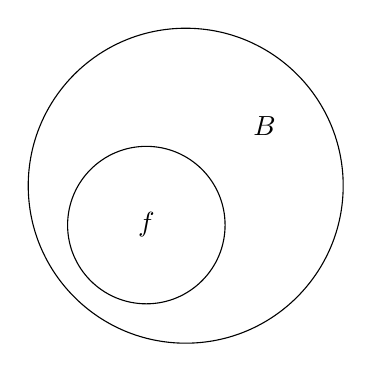
\begin{tikzpicture}
			\draw (0, 0) circle (2cm);
			\draw (-0.5, -0.5) circle (1cm);
			
			\node[below] at (1, 1) {$ B $};
			\node at (-0.5, -0.5) {$ \func{\Ran}{f} $};
		\end{tikzpicture}
	\end{center}
\end{warningbox}

\par Perlu diketahui juga bahwa fungsi $ \func{g}{x} = x + 1 $ sebenarnya ekuivalen dengan fungsi $ \func{r}{y} = y + 1 $. Variabel yang digunakan dalam suatu fungsi sebenarnya tidak terlalu penting, yang penting dalam suatu fungsi adalah aturan pemetaannya itu sendiri atau formulanya.

\begin{explbox}
	Coba cari tahu mengenai kodomain dan peta (\textit{image}) dari suatu fungsi. Apakah perbedaan antara jangkauan, kodomain, dan peta?
\end{explbox}

\par Setelah mengetahui sekilas mengenai fungsi secara umum, kita kemudian siap untuk mempelajari fungsi kuadrat. Fungsi kuadrat adalah salah satu dari banyak jenis fungsi yang memiliki bentuk umum
\begin{equation} \label{eq:222}
	\func{f}{x} = ax^{2} + bx + c
\end{equation}
dengan $ a, b, c $ semuanya bilangan real dan $ a \ne 0 $.

\par Salah satu contoh dari fungsi kuadrat adalah $ \func{f}{x} = x^{2} - 3x + 1 $. Disini, nilai $ a = 1 $, $ b = -3 $, dan $ c = 1 $. Tentunya jika titik $ \left(p, q\right) $ dilalui oleh fungsi kuadrat umum \ref{eq:222}, maka titik tersebut memenuhi $ q = ap^{2} + bp + c $.

\subsection{Grafik Fungsi Kuadrat}
	
	Grafik fungsi kuadrat adalah berupa parabola, yaitu suatu kurva pada bidang yang simetris dan berbentuk mirip seperti huruf 'U'. Dalam matematika sendiri, terdapat definisi matematis mengenai parabola ini yang melibatkan titik dan garis. Definisi tersebut tidak akan kita bahas pada buku ini. Saat ini kita cukup setuju dengan fakta bahwa fungsi kuadrat berbentuk parabola.
	
	\begin{explbox}
		Bagi pembaca yang tertarik, Anda dapat mencoba mencari definisi dari parabola dan membuktikan bahwa fungsi kuadrat sebenarnya merupakan parabola.
	\end{explbox}
	
	\par Grafik fungsi kuadrat juga sangat berkaitan erat dengan koefisien-koefisiennya (dalam fungsi kuadrat pada persamaan \ref{eq:222}, koefisien-koefisien yang dimaksud adalah $ a $, $ b $, dan $ c $). Koefisien $ a $ mengatur derajat kelengkungan grafik fungsi kuadrat; semakin besar nilai $ a $ akan memberikan grafik fungsi kuadrat yang lebih tertutup (melengkung tajam). Selain itu, koefisien $ a $ juga mengatur arah kecekungan grafik fungsi kuadrat; jika $ a > 0 $, maka grafik fungsi kuadrat tersebut akan cekung ke atas (terbuka ke atas), dan jika $ a < 0 $, maka grafik fungsi kuadrat tersebut akan cekung ke bawah (terbuka ke bawah). Hal ini akan dipelajari lebih lanjut pada mata kuliah kalkulus. Berikut merupakan ilustrasi grafik fungsi kuadrat untuk berbagai nilai $ a $.
	\begin{multicols}{2}
		\noindent
		\begin{figure}[H]
			\centering
			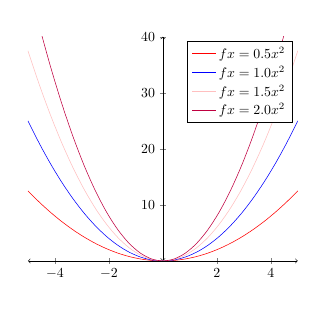
\begin{tikzpicture}[scale=0.5]
				\begin{axis}
					[axis x line=center, axis y line=center, ymax=40, axis line style={<->}]
					\addplot[smooth, red] {0.5 * x^2};
					\addplot[smooth, blue] {x^2};
					\addplot[smooth, pink] {1.5 * x^2};
					\addplot[smooth, purple] {2 * x^2};
					
					\legend{$ \func{f}{x} = 0.5x^2 $, $ \func{f}{x} = 1.0x^2 $, $ \func{f}{x} = 1.5x^2 $, $ \func{f}{x} = 2.0x^2 $};
				\end{axis}
			\end{tikzpicture}
			\caption{Grafik fungsi kuadrat $ \func{f}{x} $ untuk beberapa nilai $ a $.}
		\end{figure}
		
		\columnbreak
		
		\begin{figure}[H]
			\centering
			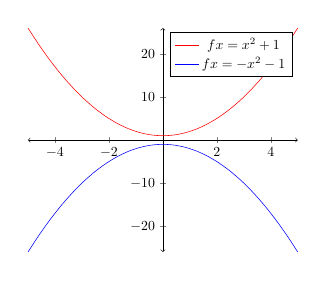
\begin{tikzpicture}[scale=0.5]
				\begin{axis}
					[axis x line=center, axis y line=center, axis line style={<->}]
					\addplot[smooth, red] {x^2 + 1};
					\addplot[smooth, blue] {-x^2 - 1};
					
					\legend{$ \func{f}{x} = x^2 + 1 $, $ \func{f}{x} = -x^2 - 1 $};
				\end{axis}
			\end{tikzpicture}
			\caption{Grafik fungsi kuadrat $ \func{f}{x} $ ketika $ a > 0 $ dan ketika $ a < 0 $.}
		\end{figure}
	\end{multicols}
	
	\par Selanjutnya pada fungsi kuadrat juga terdapat koefisien $ c $. Kita akan membahas koefisien $ b $ di akhir karena agak rumit. Perhatikan bahwa pada fungsi kuadrat umum \ref{eq:222}, jika kita substitusi $ x = 0 $, kita akan mendapatkan $ \func{f}{0} = a\left(0\right)^{2} + b\left(0\right) + c = c $. Akibatnya, $ f $ akan berpotongan dengan sumbu-$ y $ tepat pada titik $ \left(0, c\right) $. Oleh karena itu, koefisien $ c $ pada fungsi kuadrat mengatur dimana fungsi kuadrat tersebut akan berpotongan dengan sumbu-$ y $. Jika $ c > 0 $, maka fungsi kuadrat akan berpotongan dengan sumbu-$ y $ positif. Sedangkan jika $ c < 0 $, maka fungsi kuadrat akan berpotongan dengan sumbu-$ y $ negatif (bagaimana jika $ c = 0 $?). Berikut merupakan ilustrasi grafik fungsi kuadrat untuk berbagai nilai $ c $.
	\begin{figure}[H]
		\centering
		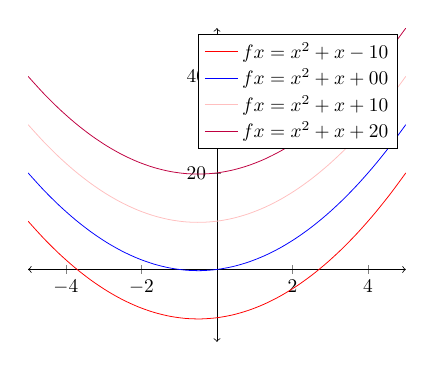
\begin{tikzpicture}[scale=0.7]
			\begin{axis}
				[axis x line=center, axis y line=center, ymin=-15, axis line style={<->}]
				\addplot[smooth, red] {x^2 + x + -10};
				\addplot[smooth, blue] {x^2 + x + 0};
				\addplot[smooth, pink] {x^2 + x + 10};
				\addplot[smooth, purple] {x^2 + x + 20};
				
				\legend{$ \func{f}{x} = x^2 + x - 10 $, $ \func{f}{x} = x^2 + x + 00 $, $ \func{f}{x} = x^2 + x + 10 $, $ \func{f}{x} = x^2 + x + 20 $};
			\end{axis}
		\end{tikzpicture}
		\caption{Grafik fungsi kuadrat $ \func{f}{x} $ untuk beberapa nilai $ c $.}
	\end{figure}
	
	\par Sama seperti persamaan kuadrat, pada fungsi kuadrat juga terdapat diskriminan, yaitu $ b^{2} - 4ac $. Diskriminan fungsi kuadrat tidak dilambangkan dengan $ D $ seperti pada persamaan kuadrat, tetapi langsung disebutkan dengan $ b^{2} - 4ac $. Diskriminan pada persamaan kuadrat memberikan kita informasi mengenai banyaknya akar persamaan kuadrat. Akar persamaan kuadrat disini adalah beberapa nilai $ x $ yang 'menghasilkan' 0 pada persamaan tersebut. Oleh karena itu, diskriminan pada fungsi kuadrat akan memberikan kita informasi mengenai banyaknya titik potong grafik fungsi kuadrat dengan sumbu-$ x $. Jika $ b^{2} - 4ac > 0 $, maka grafik fungsi kuadrat akan berpotongan dengan sumbu-$ x $ di dua titik berbeda. Sedangkan jika $ b^{2} - 4ac < 0 $, maka grafik fungsi kuadrat tidak akan berpotongan dengan sumbu-$ x $ (bagaimana jika $ b^{2} - 4ac = 0 $?). Berikut merupakan ilustrasi grafik fungsi kuadrat untuk berbagai nilai diskriminannya.
	\begin{figure}[H]
		\centering
		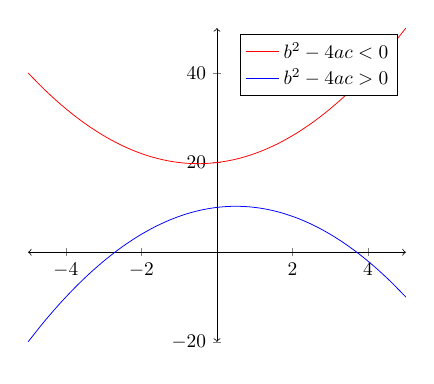
\begin{tikzpicture}[scale=0.7]
			\begin{axis}
				[axis x line=center, axis y line=center, axis line style={<->}]
				\addplot[smooth, red] {x^2 + x + 20};
				\addplot[smooth, blue] {-x^2 + x + 10};
				
				\legend{$ b^2 - 4ac < 0 $, $ b^2 - 4ac > 0 $};
			\end{axis}
		\end{tikzpicture}
		\caption{Grafik fungsi kuadrat $ \func{f}{x} $ untuk beberapa nilai $ c $.}
	\end{figure}
	
	\par Ketika fungsi kuadrat memiliki diskriminan yang bernilai positif, maka grafiknya akan berpotongan dengan sumbu-$ x $ pada dua titik berbeda. Misalkan titik-titik tersebut adalah $ \left(x_{1}, 0\right) $ dan $ \left(x_{2}, 0\right) $. Perhatikan bahwa $ x_{1} $ dan $ x_{2} $ disini adalah solusi dari persamaan $ \func{f}{x} = ax^{2} + bx + c = 0 $. Mudah dilihat bahwa jika kita menarik garis vertikal yang melalui titik tengah antara $ x_{1} $ dan $ x_{2} $, maka garis tersebut akan membagi dua grafik fungsi kuadrat menjadi dua bagian yang simetris. Garis vertikal tersebut dinamakan sumbu simetri dan biasa dinotasikan sebagai $ x_{p} $.
	\begin{figure}[H]
		\centering
		\begin{tikzpicture}
			\begin{axis}
				[ticks=none, axis x line=center, axis y line=center, xmin=-1, xmax=4, ymin=-1.5, ymax=4, axis line style={<->}]
				\addplot[smooth, red] {x^2 - 4*x + 3};
				\addplot[smooth, blue] coordinates {(2, -1.5) (2, 4)} node[below=0.5cm, right] {$ x = x_{p} $};
				
				\addplot[black, mark = *] coordinates {(1, 0)};
				\addplot[black, mark = *] coordinates {(3, 0)};
				
				\node[below left] at (axis cs:1,0) {$ x_{1} $};
				\node[below right] at (axis cs:3,0) {$ x_{2} $};
			\end{axis}
		\end{tikzpicture}
		\caption{Ilustrasi sumbu simetri pada suatu grafik fungsi kuadrat. Perhatikan bahwa sumbu simetri tersebut pastilah bernilai positif karena berada di sebelah kanan sumbu-$ y $.}
	\end{figure}
	Karena sumbu simetri melalui titik tengah $ x_{1} $ dan $ x_{2} $, maka persamaan garisnya adalah
	\begin{equation} \label{eq:223}
		x = x_{p} = \frac{x_{1} + x_{2}}{2}.
	\end{equation}
	Oleh karena itu, dengan menggunakan formula \ref{eq:210}, kita dapat menulis ulang persamaan \ref{eq:223} sebagai
	\begin{equation} \label{eq:224}
		x = x_{p} = -\frac{b}{2a}.
	\end{equation}
	Persamaan \ref{eq:224} ini akan sangat membantu untuk mengetahui sumbu simetri suatu fungsi kuadrat yang sukar difaktorkan (juga untuk fungsi kuadrat yang akar-akarnya tidak diketahui secara eksplisit). Bahkan persamaan \ref{eq:224} ini juga berlaku untuk fungsi kuadrat yang akar-akarnya takreal (mengapa?).
	
	\par Perpotongan sumbu simetri dengan grafik fungsi kuadrat disebut sebagai titik puncak atau titik ekstrim\footnote{Biasa juga disebut sebagai titik balik atau titik stasioner.}. Ada dua tipe titik ekstrim yang bergantung pada tanda dari koefisien $ a $. Jika $ a > 0 $, maka titik ekstrimnya berupa titik minimum (titik balik minimum). Sedangkan jika $ a < 0 $, maka titik ekstrimnya berupa titik maksimum (titik balik maksimum). Hal ini dapat dicek dengan menggunakan uji turunan pertama yang akan dipelajari pada mata kuliah kalkulus. Koordinat dari titik ekstrim ini adalah
	\[ \left(x_{p}, \func{f}{x_{p}}\right) \quad \mbox{atau} \quad \left(-\frac{b}{2a}, -\frac{b^{2} - 4ac}{4a}\right). \]
	Disini, $ x_{p} $ disebut sebagai absis dan $ \func{f}{x_{p}} $ disebut sebagai ordinat. Faktanya, untuk sebarang titik koordinat $ \left(u, v\right) $, $ u $ disebut sebagai absis dan $ v $ disebut sebagai ordinat.
	
	\begin{explbox}
		Coba uraikan mengapa $ \func{f}{x_{p}} = -\dfrac{b^{2} - 4ac}{4a} $.
	\end{explbox}
	
	\par Terakhir, kita akan membahas mengenai koefisien $ b $. Dari persamaan \ref{eq:224}, kita tahu bahwa koefisien $ a $ dan koefisien $ b $ bersama-sama mengontrol lokasi dari sumbu simetri (dan tentunya juga mengontrol lokasi dari absis titik ekstrim) suatu fungsi kuadrat. Dari persamaan \ref{eq:224} juga mudah didapatkan bahwa $ b = -2ax_{p} $. Oleh karena itu, jika $ a $ dan $ x_{p} $ bertanda sama, maka $ b $ akan bernilai negatif. Sedangkan jika $ a $ dan $ x_{p} $ berbeda tanda, maka $ b $ akan bernilai positif.
	
	\begin{explbox}
		Periksa apakah konvers dari pernyataan-pernyataan berikut juga benar.
		\begin{enumerate}[leftmargin=*]
			\item Jika $ a > 0 $, maka grafik fungsi kuadratnya akan cekung ke atas (terbuka ke atas).
			\item Jika $ b > 0 $, maka $ a $ dan $ x_{p} $ berbeda tanda.
			\item Jika $ c > 0 $, maka grafik fungsi kuadratnya akan memotong sumbu-$ y $ positif.
			\item Jika $ b^{2} - 4ac > 0 $, maka grafik fungsi kuadratnya akan memotong sumbu-$ x $ tepat pada dua titik berbeda.
		\end{enumerate}
	\end{explbox}
	
	\par Untuk mengakhiri bagian ini, kita akan mengerjakan beberapa contoh soal agar Anda dapat lebih memantapkan diri dalam mengerjakan soal-soal latihan yang diberikan.
	
	\begin{contoh}
		Tentukan tanda dari $ a $, $ b $, $ c $, dan $ b^{2} - 4ac $ dari grafik fungsi kuadrat berikut.
		\begin{center}
			\begin{tikzpicture}[scale=0.7]
				\begin{axis}
					[ticks=none, axis x line=center, axis y line=center, xmin=-8, xmax=5, ymin=-40, ymax=15, axis line style={<->}, legend pos=south west]
					\addplot[smooth, red, domain=-8:5] {-x^2 - (17/5)*x + 5};
					
					\legend{$ \func{f}{x} = ax^{2} + bx + c $}
				\end{axis}
			\end{tikzpicture}
		\end{center}
	\end{contoh}
	\begin{jawab}
		Karena grafik fungsinya terbuka ke bawah, maka $ a < 0 $. Karena grafik fungsinya memotong sumbu-$ y $ positif, maka $ c > 0 $. Karena grafik fungsinya memotong sumbu-$ x $ tepat di dua titik berbeda, maka $ b^{2} - 4ac > 0 $. Karena $ x_{p} < 0 $ dan $ a < 0 $, berarti $ x_{p} $ dan $ a $ bertanda sama sehingga $ b > 0 $.
	\end{jawab}
	
	\begin{contoh}
		Sketsakan grafik fungsi kuadrat $ \func{f}{x} = ax^{2} + bx + c $ jika diketahui $ a > 0 $, $ b > 0 $, $ c < 0 $, dan $ b^{2} - 4ac = 0 $.
	\end{contoh}
	\begin{jawab}
		Karena $ a > 0 $, maka $ f $ terbuka ke atas. Karena $ c < 0 $, maka $ f $ memotong sumbu-$ y $ negatif. Karena $ b^{2} - 4ac = 0 $, maka $ f $ menyinggung sumbu-$ x $ tepat di satu titik. Karena $ b > 0 $, maka $ a $ dan $ x_{p} $ berbeda tanda sehingga $ x_{p} > 0 $.
		\par Sebelum mensketsakan grafik, cermati dahulu apakah mungkin untuk mensketsakan grafik dengan kondisi yang diberikan. Perhatikan bahwa $ f $ terbuka ke atas dan memotong sumbu-$ y $ negatif. Berarti titik puncaknya (dalam hal ini titik balik minimum) haruslah berada di bawah sumbu-$ x $. Akibatnya, $ f $ memotong sumbu-$ x $ tepat di dua titik. Hal ini berkontradiksi dengan fakta bahwa $ f $ haruslah menyinggung sumbu-$ x $ tepat di satu titik.
		\par Jadi tidak mungkin ada fungsi kuadrat yang memenuhi kondisi yang diberikan sehingga tidak mungkin juga untuk mensketsakan grafiknya.
	\end{jawab}
	
	\begin{contoh}
		Sketsakan grafik fungsi kuadrat $ \func{f}{x} = 2x^{2} - 4x + 5 $.
	\end{contoh}
	\begin{jawab}
		Dengan membandingkan koefisien-koefisien fungsi kuadrat pada soal dengan fungsi kuadrat umum \ref{eq:222}, kita punyai $ a = 2 $, $ b = -4 $, dan $ c = 5 $. Karena $ a > 0 $, maka $ f $ terbuka ke atas. Karena $ c > 0 $, maka $ f $ memotong sumbu-$ y $ positif. Karena $ b^{2} - 4ac = \left(-4\right)^{2} - 4\left(2\right)\left(5\right) = -24 < 0 $, maka fungsi $ f $ tidak memotong sumbu-$ x $. Dengan menggunakan persamaan \ref{eq:224}, kita tahu bahwa sumbu simetri $ f $ adalah $ x_{p} = -\dfrac{-4}{2\left(2\right)} = 1 > 0 $. Akibatnya, $ f $ mencapai nilai minimumnya ketika $ x = 1 $. Oleh karena itu, nilai minimum dari $ f $ adalah $ \func{f}{1} = 2\left(1\right)^{2} - 4\left(1\right) + 5 = 3 $.
		\par Jadi, sketsa grafik fungsi kuadrat $ f $ adalah sebagai berikut.
		\begin{center}
			\begin{tikzpicture}[scale=0.7]
				\begin{axis}
					[axis x line=center, axis y line=center, xmin=-1, xmax=3, ymin=-1, ymax=15, extra y ticks={3}, extra y tick labels={3}, axis line style={<->}]
					\addplot[smooth, red] {2*x^2 - 4*x + 5};
					
					\legend{$ \func{f}{x} = 2x^{2} - 4x + 5 $}
				\end{axis}
			\end{tikzpicture}
		\end{center}
	\end{jawab}

\subsection{Menentukan Fungsi Kuadrat}
	
	Kita telah mengetahui bahwa fungsi kuadrat memiliki bentuk umum seperti pada persamaan \ref{eq:222}. Bentuk umum ini biasa disebut sebagai bentuk standar fungsi kuadrat. Kita selalu bisa memfaktorkan ruas kanan persamaan \ref{eq:222}, terlepas dari kemungkinan sukarnya pemfaktoran untuk dilakukan. Jika $ x_{1} $ dan $ x_{2} $ adalah akar-akar dari fungsi kuadrat umum \ref{eq:222}, maka kita dapat tulis ulang $ \func{f}{x} $ sebagai
	\begin{equation} \label{eq:225}
		\func{f}{x} = a\left(x - x_{1}\right)\left(x - x_{2}\right).
	\end{equation}
	Bentuk ini biasa disebut sebagai bentuk terfaktorkan fungsi kuadrat. Akan sangat mudah untuk menentukan fungsi kuadrat apabila telah diketahui lokasi akar-akarnya dan satu titik lainnya dengan menggunakan persamaan \ref{eq:225} ini. Jika hanya diketahui lokasi akar-akarnya saja tentunya masih belum cukup untuk menentukan fungsi kuadratnya, karena masih ada konstanta $ a $ yang belum diketahui. Kita akan mengerjakan beberapa contoh soal untuk lebih memahami mengenai hal ini.
	
	\begin{contoh}
		Tentukan fungsi kuadrat yang melalui titik $ \left(-3, 12\right) $ dan memotong sumbu-$ x $ di titik $ \left(1, 0\right) $ dan $ \left(-2, 0\right) $.
	\end{contoh}
	\begin{jawab}
		Misalkan fungsi kuadrat yang memenuhi adalah $ \func{f}{x} $. Karena $ f $ memotong sumbu-$ x $ di titik $ \left(1, 0\right) $ dan $ \left(-2, 0\right) $, maka $ f $ memiliki akar-akar $ x_{1} = 1 $ dan $ x_{2} = -2 $. Oleh karena itu, dengan menggunakan persamaan \ref{eq:225}, kita punyai
		\[ \func{f}{x} = a\left(x - 1\right)\left(x + 2\right). \]
		Karena $ f $ melalui titik $ \left(-3, 12\right) $, maka $ f $ memenuhi
		\[ \func{f}{-3} = 12 \iff a\left(-3 - 1\right)\left(-3 + 2\right) = 12 \iff \left(-4\right)\left(-1\right)a = 12 \iff a = 3. \]
		Jadi, fungsi kuadrat yang memenuhi adalah
		\[ \func{f}{x} = 3\left(x - 1\right)\left(x + 2\right) = 3x^{2} + 3x - 6. \]
	\end{jawab}
	
	\begin{contoh}
		Tentukan fungsi kuadrat yang bernilai negatif untuk $ -2 < x < 3 $ dan melalui titik $ \left(1, -6\right) $.
	\end{contoh}
	\begin{jawab}
		Soal ini mungkin agak mengintimidasi pada awal ketika kita membacanya. Tetapi, jika kita memperhatikan lebih lanjut mengenai grafik fungsi kuadrat, kita akan dapat dengan mudah menyelesaikannya. Ingat kembali bahwa berdasarkan tanda koefisien $ a $ pada fungsi kuadrat umum \ref{eq:222}, maka terdapat dua kemungkinan grafik dari suatu fungsi kuadrat, yaitu terbuka ke atas atau terbuka ke bawah. Ilustrasinya adalah sebagai berikut.
		\begin{figure}[H]
			\centering
			\begin{multicols}{2}
				\noindent
				\begin{tikzpicture}[scale=0.7]
					\begin{axis}
						[ticks=none, axis x line=center, axis y line=none, ymin=-5, ymax=5, axis line style={<->}]
						\addplot[smooth, red] {x^2 - 4};
						
						\legend{$ a > 0 $}
					\end{axis}
				\end{tikzpicture}
				
				\columnbreak
				
				\begin{tikzpicture}[scale=0.7]
					\begin{axis}
						[ticks=none, axis x line=center, axis y line=none, ymin=-5, ymax=5, axis line style={<->}]
						\addplot[smooth, red] {-x^2 + 4};
						
						\legend{$ a < 0 $}
					\end{axis}
				\end{tikzpicture}
			\end{multicols}
			\caption{Dua kemungkinan grafik fungsi kuadrat berdasarkan tanda koefisien $ a $.}
		\end{figure}
		Perhatikan bahwa perpotongan grafik fungsi kuadrat pada gambar ilustrasi di atas dengan sumbu-$ x $ adalah akar-akar dari fungsi kuadrat tersebut. Misalkan akar-akarnya adalah $ x_{1} $ dan $ x_{2} $ dengan $ x_{1} < x_{2} $. Oleh karena itu, pada gambar sebelah kiri, fungsi kuadrat tersebut akan bernilai negatif untuk $ x_{1} < x < x_{2} $, dan bernilai positif untuk $ x < x_{1} $ atau $ x > x_{2} $. Selain itu, pada gambar sebelah kanan, fungsi kuadrat tersebut akan bernilai positif untuk $ x_{1} < x < x_{1} $, dan bernilai negatif untuk $ x < x_{1} $ atau $ x > x_{2} $.
		\par Dengan pemahaman mengenai hal ini, kita akan dapat dengan mudah mengerjakan soal ini. Misalkan fungsi kuadrat yang memenuhi kondisi pada soal adalah $ \func{f}{x} $. Karena $ f $ bernilai negatif untuk $ -2 < x < 3 $, maka dari ilustrasi di atas, grafik fungsi $ f $ yang mungkin adalah grafik sebelah kiri. Oleh karena itu, koefisien $ a $ pada fungsi kuadrat $ f $ bernilai positif. Lebih jauh, akar-akar dari fungsi $ f $ adalah $ x_{1} = -2 $ dan $ x_{2} = 3 $. Oleh karena itu, kita punyai
		\[ \func{f}{x} = a\left(x + 2\right)\left(x - 3\right). \]
		Sampai disini proses pencarian $ a $ sama seperti contoh sebelumnya dan diserahkan kepada pembaca.
	\end{jawab}
	
	\par Selain memiliki bentuk terfaktorkan, ternyata fungsi kuadrat umum \ref{eq:222} juga memiliki bentuk lainnya yang bergantung pada lokasi titik ekstrim. Bentuk ini dinamakan bentuk titik puncak (\textit{vertex form}). Kita dapat dengan mudah mendapatkan bentuk ini dari bentuk umumnya dengan melengkapkan kuadrat. Perhatikan bahwa bentuk umum \ref{eq:222} dapat ditulis ulang sebagai
	\begin{align*}
		\func{f}{x} &= ax^{2} + bx + c \\
		&= a\left(x^{2} + \frac{b}{a}x + \frac{c}{a}\right) \\
		&= a\left(x^{2} + 2 \cdot \frac{b}{2a}x + \frac{b^{2}}{4a^{2}} - \frac{b^{2}}{4a^{2}} + \frac{c}{a}\right) \\
		&= a\left(x^{2} + 2 \cdot \frac{b}{2a}x + \frac{b^{2}}{4a^{2}}\right) - \frac{b^{2}}{4a} + c \\
		&= a\left(x + \frac{b}{2a}\right)^{2} - \frac{b^{2} - 4ac}{4a}
	\end{align*}
	Padahal kita punyai
	\[ x_{p} = -\frac{b}{2a} \quad \mbox{dan} \quad \func{f}{x_{p}} = -\dfrac{b^{2} - 4ac}{4a}. \]
	Oleh karena itu, kita dapat tulis ulang hasil yang kita dapatkan sebagai
	\[ \func{f}{x} = a\left(x - x_{p}\right)^{2} + \func{f}{x_{p}}. \]
	Disini, $ \func{f}{x_{p}} $ biasa dituliskan sebagai $ y_{p} $ sehingga
	\begin{equation} \label{eq:226}
		\func{f}{x} = a\left(x - x_{p}\right)^{2} + y_{p}.
	\end{equation}
	Bentuk inilah yang disebut sebagai bentuk titik puncak fungsi kuadrat. Akan sangat mudah untuk menentukan fungsi kuadrat apabila telah diketahui lokasi titik puncaknya dan satu titik lainnya dengan menggunakan persamaan \ref{eq:226} ini. Jika hanya diketahui lokasi titik puncaknya saja tentunya masih belum cukup untuk menentukan fungsi kuadratnya, karena masih ada konstanta $ a $ yang belum diketahui. Kita akan mengerjakan beberapa contoh soal untuk lebih memahami mengenai hal ini.
	
	\begin{contoh}
		Tentukan fungsi kuadrat yang memiliki titik ekstrim $ \left(3, 9\right) $ dan melalui titik $ \left(1, 5\right) $.
	\end{contoh}
	\begin{jawab}
		Misalkan fungsi kuadrat yang memenuhi adalah $ \func{f}{x} $. Karena $ f $ memiliki titik ekstrim $ \left(3, 9\right) $, maka $ x_{p} = 3 $ dan $ \func{f}{x_{p}} = y_{p} = 9 $. Oleh karena itu, dengan menggunakan persamaan \ref{eq:226} kita punyai
		\[ \func{f}{x} = a\left(x - 3\right)^{2} + 9. \]
		Karena $ f $ juga melalui titik $ \left(1, 5\right) $, maka $ f $ memenuhi
		\[ \func{f}{1} = 5 \iff a\left(1 - 3\right)^{2} + 9 = 5 \iff 4a = -4 \iff a = -1. \]
		Jadi, fungsi kuadrat yang memenuhi adalah
		\[ \func{f}{x} = -\left(x - 3\right)^{2} + 9 = -x^{2} + 6x. \]
	\end{jawab}
	
	\par Setelah mempelajari dua bentuk fungsi kuadrat selain bentuk umumnya, kita sudah semakin yakin untuk menentukan fungsi kuadrat dengan mudah. Jika diketahui lokasi-lokasi akar dan satu titik lain, bisa digunakan persamaan \ref{eq:225} untuk menentukan fungsi kuadrat yang berkaitan. Selain itu, jika diketahui lokasi titik puncak dan satu titik lain, bisa digunakan persamaan \ref{eq:226} untuk menentukan fungsi kuadrat yang berkaitan. Tetapi kemudian muncul permasalahan baru. Bagaimana cara menentukan fungsi kuadrat yang tidak diketahui lokasi akar-akarnya ataupun lokasi titik puncaknya, tetapi hanya diketahui titik-titik yang dilaluinya? Mudah saja, kita hanya tinggal menggunakan bentuk umum fungsi kuadrat seperti pada persamaan \ref{eq:222} untuk kemudian ditentukan nilai dari koefisien $ a $, $ b $, dan $ c $. Tentunya karena ada tiga koefisien yang harus dicari, maka harus diketahui juga tiga titik berbeda yang dilalui oleh suatu fungsi kuadrat. Hal ini dikarenakan jika diketahui tiga titik, maka akan terbentuk sistem persamaan linear tiga variabel yang dapat diselesaikan. Sebagai contoh, kita akan mengerjakan soal berikut.
	
	\begin{contoh}
		Tentukan fungsi kuadrat yang melalui titik-titik $ \left(1, 2\right) $, $ \left(-1, 4\right) $, dan $ \left(3, 8\right) $.
	\end{contoh}
	\begin{jawab}
		Misalkan fungsi kuadrat yang memenuhi adalah $ \func{f}{x} $. Oleh karena itu, dengan menggunakan persamaan \ref{eq:222} kita punyai
		\[ \func{f}{x} = ax^{2} + bx + c. \]
		Karena $ f $ melalui $ \left(1, 2\right) $, $ \left(-1, 4\right) $, dan $ \left(3, 8\right) $, maka kita akan mendapatkan sistem persamaan
		\begin{center}
			\systeme{
				a + b + c = 2,
				a - b + c = 4,
				9a + 3b + c = 8
			}
		\end{center}
		yang jika diselesaikan akan didapatkan $ a = 1 $, $ b = -1 $, dan $ c = 2 $. Akibatnya, fungsi kuadrat yang memenuhi adalah
		\[ \func{f}{x} = x^{2} - x + 2. \]
	\end{jawab}
	
\subsection{Domain dan Jangkauan Fungsi Kuadrat}
	
	Secara umum, untuk sebarang fungsi kuadrat $ \func{f}{x} $, domainnya adalah himpunan bilangan real dan jangkauannya bergantung pada letak titik puncak beserta nilai dari koefisien $ a $-nya. Jika $ a > 0 $, maka fungsi $ f $ akan mencapai titik minimum di $ \left(x_{p}, y_{p}\right) $ sehingga jangkauannya adalah $ \func{\Ran}{f} = \set{\func{f}{x} \in \mathbb{R}}{\func{f}{x} \geq y_{p}} $. Sedangkan jika $ a < 0 $, maka $ f $ akan mencapai titik maksimum di $ \left(x_{p}, y_{p}\right) $ sehingga jangkauannya adalah $ \func{\Ran}{f} = \set{\func{f}{x} \in \mathbb{R}}{\func{f}{x} \leq y_{p}} $. Agar lebih jelas, kita akan mengerjakan contoh berikut.
	
	\begin{contoh}
		Tentukan domain dan jangkauan dari fungsi $ \func{f}{x} = x^{2} - 2x + 3 $.
	\end{contoh}
	\begin{jawab}
		Jelas bahwa fungsi $ f $ dapat menerima input untuk setiap bilangan real $ x $ sehingga domain dari fungsi $ f $ adalah $ \func{\Dom}{f} = \mathbb{R} $. Perhatikan bahwa karena koefisien $ x^{2} $ pada fungsi $ f $ lebih besar daripada nol, maka $ f $ akan mencapai titik minimum ketika $ x = x_{p} = -\dfrac{-2}{2\left(1\right)} = 1 $. Oleh karena itu, nilai minimum dari $ f $ adalah $ \func{f}{x_{p}} = \func{f}{1} = 1^{2} - 2\left(1\right) + 3 = 2 $. Sketsa grafik fungsi $ f $ adalah sebagai berikut (cek!).
		\begin{center}
			\begin{tikzpicture}[scale=0.7]
				\begin{axis}
					[axis x line=center, axis y line=center, xmin=-1, xmax=3, ymin=-1, ymax=6, extra y ticks={3}, extra y tick labels={3}, axis line style={<->}]
					\addplot[smooth, red] {x^2 - 2*x + 3};
					
					\legend{$ \func{f}{x} = x^{2} - 2x + 3 $}
				\end{axis}
			\end{tikzpicture}
		\end{center}
		Jika kita lihat sketsa grafiknya, maka nilai dari $ \func{f}{x} $ akan selalu lebih besar dari atau sama dengan $ \func{f}{x_{p}} = \func{f}{1} = 2 $. Inilah alasan mengapa jangkauan dari fungsi kuadrat dengan $ a > 0 $ selalu lebih besar dari atau sama dengan $ y_{p} $ atau nilai minimumnya. Oleh karena itu, jangkauan dari fungsi $ f $ adalah $ \func{\Ran}{f} = \set{\func{f}{x} \in \mathbb{R}}{\func{f}{x} \geq 2} $.
		\par Jadi, domain dan jangkaun dari fungsi $ f $ berturut-turut adalah $ \func{\Dom}{f} = \mathbb{R} $ dan $ \func{\Ran}{f} = \set{\func{f}{x} \in \mathbb{R}}{\func{f}{x} \geq 2} $.
	\end{jawab}
	
	\par Apabila domain fungsi kuadrat $ \func{f}{x} $ dibatasi, kita harus bekerja dengan lebih keras untuk mendapatkan jangkauannya. Disini kita perkenalkan istilah \textit{titik kritis}. Titik kritis adalah calon titik maksimum atau calon titik minimum (calon titik ekstrim). Untuk mengetahui jangkauan dari fungsi kuadrat yang domainnya dibatasi, kita harus mengecek titik-titik kritisnya terlebih dahulu untuk mencari nilai maksimum dan nilai minimumnya. Dalam fungsi kuadrat, titik-titik kritisnya adalah titik ujung interval dan titik baliknya. Setelah dicari titik-titik kritisnya, kita kemudian mencari manakah titik kritis yang menghasilkan nilai maksimum dan nilai minimum. Agar lebih jelas, kita akan mengerjakan beberapa contoh berikut.
	
	\begin{contoh}
		Untuk $ 1 \leq x \leq 4 $, tentukan jangkauan dari fungsi $ \func{f}{x} = 2x^{2} - 4x - 3 $.
	\end{contoh}
	\begin{jawab}
		Disini, $ 1 \leq x \leq 4 $ merupakan domain dari fungsi $ f $. Titik-titik kritisnya adalah $ \left(1, \func{f}{1}\right) $ dan $ \left(4, \func{f}{4}\right) $ yang merupakan titik ujungnya, serta $ \left(x_{p}, \func{f}{x_{p}}\right) $ yang merupakan titik balik minimumnya mengingat $ a = 2 > 0 $. Perhatikan bahwa $ x_{p} = -\dfrac{-4}{2\left(2\right)} = 1 $ sehingga $ x_{p} \in \func{\Dom}{f} $ yang kebetulan juga merupakan salah satu absis titik ujung. Berarti kita juga harus cek juga titik balik minimumnya.
		\par Kita punyai $ \func{f}{1} = -5 $, $ \func{f}{4} = 13 $, dan $ \func{f}{x_{p}} = \func{f}{1} = -5 $. Oleh karena itu, nilai minimum $ f $ dan nilai maksimum $ f $ untuk $ 1 \leq x \leq 4 $ berturut-turut adalah $ -5 $ dan 13.
		\par Jadi, jangkauan dari fungsi $ f $ adalah $ \func{\Ran}{f} = \set{\func{f}{x} \in \mathbb{R}}{-5 \leq \func{f}{x} \leq 13} $.
	\end{jawab}
	
	\begin{contoh}
		Untuk $ 0 < x \leq 5 $, tentukan jangkauan dari fungsi $ \func{f}{x} = -x^{2} - 3x + 1 $.
	\end{contoh}
	\begin{jawab}
		Karena salah satu titik ujungnya bukan merupakan domain dari fungsi $ f $, yaitu $ 0 \notin \func{\Dom}{f} $, maka $ \func{f}{0} $ tidak terdefinisi. Untuk mengatasi hal ini, kita dapat mendefinisikan fungsi $ g $ sebagai $ \func{g}{x} = -x^{2} - 3x + 1 $ untuk $ 0 \leq x \leq 5 $.
		\par Perhatikan bahwa titik-titik kritis fungsi $ g $ adalah $ \left(0, \func{g}{0}\right) $, $ \left(5, \func{g}{5}\right) $ yang merupakan titik ujungnya. Karena absis titik balik maksimum fungsi $ g $ adalah $ x_{p} = -\dfrac{-3}{2\left(-1\right)} = -\dfrac{3}{2} \notin \func{\Dom}{g} $, maka kita tidak perlu mengecek titik balik maksimumnya.
		\par Kita punyai $ \func{g}{0} = 1 $ dan $ \func{g}{5} = -39 $. Oleh karena itu, nilai minimum $ g $ dan nilai maksimum $ g $ untuk $ 0 \leq x \leq 5 $ berturut-turut adalah $ -39 $ dan 1. Akibatnya, jangkauan dari fungsi $ g $ adalah $ \func{\Ran}{g} = \set{\func{g}{x} \in \mathbb{R}}{-39 \leq \func{g}{x} \leq 1} $.
		\par Karena $ x = 0 $ tidak termasuk dalam domain fungsi $ f $, maka nilai dari $ f $ akan selalu kurang dari $ \func{g}{0} = 1 $ sehingga jangkauan fungsi $ f $ adalah $ \func{\Ran}{f} = \set{\func{f}{x} \in \mathbb{R}}{-39 \leq \func{f}{x} < 1} $ dan kita selesai.
	\end{jawab}
	
	\par Pada kasus khusus ketika jangkauan fungsi kuadrat $ \func{f}{x} $ merupakan himpunan bagian dari himpunan bilangan real positif, atau merupakan himpunan bagian dari himpunan bilangan real negatif (seperti interval $ \left[2, 10\right] $ atau $ \lbrk{-4, -1} $, tetapi tidak untuk $ \lkrb{-3, 10} $), maka kita juga akan bisa mencari jangkauan dari fungsi $ \left(\func{f}{x}\right)^{n} $ untuk $ n \in \mathbb{Z} \backslash \lrbr{0} $. Sebagai contoh, jika diketahui $ \func{\Ran}{f} = \set{\func{f}{x} \in \mathbb{R}}{1 \leq \func{f}{x} < 5} $, maka kita bisa mengetahui jangkauan dari fungsi $ \func{g}{x} = \dfrac{1}{\func{f}{x}} $. Mengingat $ 1 \leq \func{f}{x} < 5 $, maka dengan aturan ketaksamaan pada bab 3, kita punyai
	\[ \frac{1}{5} < \frac{1}{\func{f}{x}} \leq 1 \iff \frac{1}{5} < \func{g}{x} \leq 1 \]
	sehingga jangkauan dari fungsi $ \func{g}{x} $ adalah $ \func{\Ran}{g} = \set{\func{g}{x} \in \mathbb{R}}{\dfrac{1}{5} < \func{g}{x} \leq 1} $.
	
	\par Khusus untuk bilangan genap positif $ n $, jangkauan dari fungsi kuadrat $ \func{f}{x} $ diperbolehkan mengandung nol, asalkan selain nol tersebut, anggota yang lainnya tidak ada yang berbeda tanda, seperti interval $ \left[0, 1\right] $ atau $ \lbrk{-5, 0} $. Sebagai contoh, jika diketahui $ \func{\Ran}{f} = \set{\func{f}{x} \in \mathbb{R}}{0 \leq \func{f}{x} \leq 2} $, maka kita juga bisa mengetahui jangkauan dari fungsi $ \func{g}{x} = \left(\func{f}{x}\right)^{2} $. Mengingat $ 0 \leq \func{f}{x} \leq 2 $, maka dengan aturan ketaksamaan pada bab 3, kita dapat mengkuadratkan ketiga ruas sehingga akan didapatkan
	\[ 0^{2} \leq \left(\func{f}{x}\right)^{2} \leq 2^{2} \iff 0 \leq \func{g}{x} \leq 4. \]
	Oleh karena itu, jangkauan dari fungsi $ \func{g}{x} $ adalah $ \func{\Ran}{g} = \set{\func{g}{x} \in \mathbb{R}}{0 \leq \func{g}{x} \leq 4} $.
	
	\begin{explbox}
		Bagaimana dengan bilangan ganjil positif $ n $? Tentukan syarat-syarat bagi jangkauan fungsi kuadrat $ \func{f}{x} $ agar jangkauan dari fungsi $ \left(\func{f}{x}\right)^{n} $ dapat diketahui hanya dari jangkauan fungsi kuadrat $ \func{f}{x} $.
	\end{explbox}
	
	\par Anda tidak bisa mencari jangkauan dari fungsi $ \left(\func{f}{x}\right)^{n} $ untuk $ n \in \mathbb{Z} $ hanya dengan menggunakan jangkauan dari fungsi kuadrat $ \func{f}{x} $ apabila jangkauan dari fungsi kuadrat $ \func{f}{x} $ memiliki anggota yang berbeda tanda (seperti interval $ \left(-2, 6\right) $ atau $ \left[-4, 2\right] $). Untuk mencarinya, Anda perlu menggunakan bantuan kalkulus yang tentunya tidak akan kita bahas di sini. Oleh karena itu, Anda harus cermat dalam melihat jangkauan fungsi $ f $ ini. Jika terdapat soal dalam buku ini dimana diketahui $ \func{\Ran}{f} $ mengandung anggota-anggota yang berbeda tanda, cukup Anda jawab dengan "jangkauan dari fungsi $ \left(\func{f}{x}\right)^{n} $ tidak dapat diketahui hanya dengan jangkauan fungsi $ f $".
	
	\begin{explbox}
		Mengapa harus menggunakan bantuan kalkulus? Mengapa tidak digunakan saja aturan ketaksamaan untuk mencarinya?
	\end{explbox}

\subsection{Definit Positif dan Definit Negatif}
	
	Dalam fungsi kuadrat, bahkan juga sebarang fungsi selain fungsi kuadrat, terdapat istilah \textit{definit}. Secara bahasa, definit sendiri berarti 'selalu'. Oleh karena itu, definit positif berarti selalu positif dan definit negatif berarti selalu negatif.
	
	\par Jika kita menggambar grafik fungsi kuadrat yang selalu positif, maka grafiknya akan selalu berada di atas sumbu-$ x $. Berikut merupakan ilustrasinya.
	\begin{figure}[H]
		\centering
		\begin{tikzpicture}[scale=0.7]
			\begin{axis}
				[ticks=none, axis x line=center, axis y line=none, xmin=-3, xmax=3, ymin=0, ymax=6, axis line style={<->}]
				\addplot[smooth, red] {x^2 + 1};
			\end{axis}
		\end{tikzpicture}
		\caption{Ilustrasi fungsi kuadrat yang selalu positif (definit positif).}
	\end{figure}
	Perhatikan bahwa agar suatu fungsi kuadrat umum seperti pada persamaan \ref{eq:222} definit positif, maka diskriminannya harus negatif agar tidak menyinggung ataupun memotong sumbu-$ x $. Tetapi syarat tersebut masih belum cukup karena bisa saja grafik fungsinya selalu di bawah sumbu-$ x $. Oleh karena itu, agar terjamin grafik fungsinya selalu berada di atas sumbu-$ x $, nilai dari koefisien $ a $ haruslah positif. Jadi, syarat-syarat agar suatu fungsi kuadrat definit positif adalah
	\begin{equation} \label{eq:227}
		b^{2} - 4ac < 0 \quad \mbox{dan} \quad a > 0.
	\end{equation}
	
	\par Selain bisa selalu bernilai positif, suatu fungsi kuadrat juga bisa selalu bernilai negatif. Jika kita menggambar grafik fungsi kuadrat yang selalu negatif, maka grafiknya akan selalu berada di bawah sumbu-$ x $. Berikut merupakan ilustrasinya.
	\begin{figure}[H]
		\centering
		\begin{tikzpicture}[scale=0.7]
			\begin{axis}
				[ticks=none, axis x line=center, axis y line=none, xmin=-3, xmax=3, ymin=-6, ymax=0, axis line style={<->}]
				\addplot[smooth, red] {-x^2 - 1};
			\end{axis}
		\end{tikzpicture}
		\caption{Ilustrasi fungsi kuadrat yang selalu negatif (definit negatif).}
	\end{figure}
	Perhatikan bahwa agar suatu fungsi kuadrat umum seperti pada persamaan \ref{eq:222} definit negatif, maka diskriminannya harus negatif agar tidak menyinggung ataupun memotong sumbu-$ x $. Tetapi syarat tersebut masih belum cukup karena bisa saja grafik fungsinya selalu di atas sumbu-$ x $. Oleh karena itu, agar terjamin grafik fungsinya selalu berada di bawah sumbu-$ x $, nilai dari koefisien $ a $ haruslah negatif. Jadi, syarat-syarat agar suatu fungsi kuadrat definit negatif adalah
	\begin{equation} \label{eq:228}
		b^{2} - 4ac < 0 \quad \mbox{dan} \quad a < 0.
	\end{equation}
	
	\begin{explbox}
		Tentukan syarat agar suatu fungsi kuadrat selalu taknegatif. Bagaimana juga syarat agar fungsi kuadrat tersebut selalu takpositif?
	\end{explbox}
	
	\begin{contoh}
		Tentukan apakah fungsi-fungsi kuadrat di bawah definit positif atau definit negatif, atau tidak keduanya.
		\begin{enumerate}
			\item $ \func{f}{x} = 3x^{2} - 2x + 1 $
			\item $ \func{f}{x} = -x^{2} - 4x + 10 $
			\item $ \func{f}{x} = -7x^{2} + 3x - 1 $
			\item $ \func{f}{x} = x^{2} + 2x + 1 $
			\item $ \func{f}{x} = ax^{2} - 3x + 1 $ untuk $ a > 5 $
		\end{enumerate}
	\end{contoh}
	\begin{jawab}
		Untuk masing-masing fungsi, kita hitung terlebih dahulu diskriminannya. Jika diskriminannya nonnegatif, kita tidak perlu lagi lebih jauh menghitung karena sudah pasti fungsi tersebut tidak definit (baik definit positif maupun definit negatif).
		\begin{enumerate}
			\item Perhatikan bahwa $ b^{2} - 4ac = \left(-2\right)^{2} - 4\left(3\right)\left(1\right) = -8 < 0 $ dan $ a = 3 > 0 $. Oleh karena itu, $ f $ definit positif.
			\item Perhatikan bahwa $ b^{2} - 4ac = \left(-4\right)^{2} - 4\left(-1\right)\left(10\right) = 20 \geq 0 $ sehingga $ f $ tidak definit.
			\item Perhatikan bahwa $ b^{2} - 4ac = 3^{2} - 4\left(-7\right)\left(-1\right) = -19 < 0 $ dan $ a = -7 < 0 $. Oleh karena itu $ f $ definit negatif.
			\item Perhatikan bahwa $ b^{2} - 4ac = 2^{2} - 4\left(2\right)\left(1\right) = 0 \geq 0 $ sehingga $ f $ tidak definit.
			\item Perhatikan bahwa $ b^{2} - 4ac = \left(-3\right)^{2} - 4a\left(1\right) = 9 - 4a $. Karena $ a > 5 $, maka mengalikan kedua ruas dengan $ -4 $ akan didapatkan $ -4a < -20 $. Kemudian, jika kita jumlahkan kedua ruas dengan 9 akan didapatkan $ 9 - 4a < -11 $. Jadi $ b^{2} - 4ac < 0 $ dan $ a > 5 > 0 $ sehingga $ f $ definit positif.
		\end{enumerate}
	\end{jawab}
	
	\begin{contoh}
		Tentukan nilai $ m $ agar fungsi kuadrat $ \func{f}{x} = mx^{2} - x + 1 $
		\begin{enumerate}
			\item definit positif.
			\item definit negatif.
		\end{enumerate}
	\end{contoh}
	\begin{jawab}
		Kita cari dahulu diskriminannya. Perhatikan bahwa $ b^{2} - 4ac = \left(-1\right)^{2} - 4m\left(1\right) = 1 - 4m $. Selanjutnya, kita akan mengerjakan soal ini.
		\begin{enumerate}
			\item Agar $ f $ definit positif, maka $ b^{2} - 4ac = 1 - 4m < 0 \iff m > 1/4 $ dan $ a = m > 0 $. Jadi haruslah $ m \in \left(1/4, +\infty\right) $.
			\item Agar $ f $ definit negatif, maka $ b^{2} - 4ac = 1 - 4m < 0 \iff m > 1/4 $ dan $ a = m < 0 $. Tetapi tidak akan ada perpotongan dari kedua interval tersebut. Oleh karena itu, tidak ada $ m $ yang membuat $ f $ definit negatif. Dengan kata lain, $ m \in \emptyset $.
		\end{enumerate}
	\end{jawab}
	
\subsection{Kedudukan Fungsi Kuadrat Terhadap Fungsi Lainnya}
	
	Terdapat tiga kemungkinan kedudukan fungsi kuadrat terhadap fungsi lainnya. Kemungkinan-kemungkinannya adalah fungsi kuadrat tersebut berpotongan terhadap fungsi lainnya, menyinggung fungsi lainnya, dan tidak menyingggung maupun memotong fungsi lainnya. Dalam materi ini, yang dimaksud dengan fungsi lainnya hanya terbatas pada fungsi kuadrat dan fungsi linear.
	
	\subsubsection{Kedudukan Fungsi Kuadrat Terhadap Fungsi Linear}
	
		\par Misalkan diberikan fungsi kuadrat $ \func{f}{x} $ dan fungsi linear $ \func{g}{x} $. Agar kedua fungsi tersebut saling berpotongan tepat di dua titik, maka haruslah terdapat dua nilai $ x $ yang memenuhi $ \func{f}{x} = \func{g}{x} $. Tetapi persamaan tersebut tentunya ekuivalen dengan $ \func{f}{x} - \func{g}{x} = 0 $. Perhatikan bahwa pengurangan fungsi kuadrat dengan fungsi linear akan tetap menghasilkan fungsi kuadrat. Oleh karena itu, misalkan $ \func{h}{x} = \func{f}{x} - \func{g}{x} $. Agar persamaan kuadrat $ \func{h}{x} = 0 $ memiliki dua solusi real $ x $, haruslah diskriminan persamaan tersebut bernilai positif.
		\begin{figure}[H]
			\centering
			\begin{tikzpicture}[scale=0.6]
				\begin{axis}
					[ticks=none, axis x line=none, axis y line=none, xmin=-3.5, xmax=3.5, ymin=-1.5, ymax=3.5, axis line style={<->}, legend pos=south east]
					\addplot[smooth, red] {x^2};
					\addplot[smooth, blue] {0.5*x + 1};
					
					\legend{$ \func{f}{x} $, $ \func{g}{x} $}
				\end{axis}
			\end{tikzpicture}
			\caption{Ilustrasi fungsi kuadrat $ \func{f}{x} $ dan fungsi linear $ \func{g}{x} $ yang berpotongan di dua titik.}
		\end{figure}
		
		\par Dengan cara serupa, agar fungsi kuadrat $ \func{f}{x} $ dan fungsi linear $ \func{g}{x} $ saling bersinggungan, maka diskriminan persamaan $ \func{h}{x} = 0 $ haruslah sama dengan nol.
		\begin{figure}[H]
			\centering
			\begin{tikzpicture}[scale=0.6]
				\begin{axis}
					[ticks=none, axis x line=none, axis y line=none, xmin=-3.5, xmax=3.5, ymin=-1.5, ymax=3.5, axis line style={<->}, legend pos=south east]
					\addplot[smooth, red] {x^2};
					\addplot[smooth, blue] {0.5*x - 0.0625};
					
					\legend{$ \func{f}{x} $, $ \func{g}{x} $}
				\end{axis}
			\end{tikzpicture}
			\caption{Ilustrasi fungsi kuadrat $ \func{f}{x} $ dan fungsi linear $ \func{g}{x} $ yang saling bersinggungan.}
		\end{figure}
		Selain itu, agar fungsi kuadrat $ \func{f}{x} $ dan fungsi linear $ \func{g}{x} $ tidak menyinggung maupun memotong satu sama lain, maka diskriminan persamaan $ \func{h}{x} = 0 $ haruslah kurang dari nol.
		\begin{figure}[H]
			\centering
			\begin{tikzpicture}[scale=0.6]
				\begin{axis}
					[ticks=none, axis x line=none, axis y line=none, xmin=-3.5, xmax=3.5, ymin=-1.5, ymax=3.5, axis line style={<->}, legend pos=south east]
					\addplot[smooth, red] {x^2};
					\addplot[smooth, blue] {0.5*x - 0.5};
					
					\legend{$ \func{f}{x} $, $ \func{g}{x} $}
				\end{axis}
			\end{tikzpicture}
			\caption{Ilustrasi fungsi kuadrat $ \func{f}{x} $ dan fungsi linear $ \func{g}{x} $ yang tidak berpotongan ataupun bersinggungan.}
		\end{figure}
		Agar lebih jelas, kita akan mengerjakan beberapa contoh berikut.
		
		\begin{contoh}
			Tentukan kedudukan fungsi kuadrat $ \func{f}{x} = x^{2} - 2x + 3 $ dengan fungsi $ \func{g}{x} = 2x - 1 $. Jika kedua fungsi tersebut berpotongan atau bersinggungan, tentukan titik potongnya atau titik singgungnya.
		\end{contoh}
		\begin{jawab}
			Perhatikan bahwa $ \func{f}{x} - \func{g}{x} = x^{2} - 2x + 3 - \left(2x - 1\right) = x^{2} - 4x + 4 $. Karena diskriminan persamaan $ x^{2} - 4x + 4 = 0 $ adalah $ D = \left(-4\right)^{2} - 4\left(1\right)\left(4\right) = 0 $, maka fungsi kuadrat $ f $ menyinggung fungsi $ g $.
			\par Lebih jauh, jika kita menyelesaikan persamaan $ x^{2} - 4x + 4 = 0 $, maka kita akan dapat menentukan lokasi titik singgung kedua persamaan tersebut. Perhatikan bahwa
			\[ x^{2} - 4x + 4 = 0 \iff \left(x - 2\right)^{2} = 0 \]
			sehingga $ x = 2 $. Oleh karena itu, titik singgung kedua persamaan tersebut adalah $ \left(2, \func{f}{2}\right) $ atau $ \left(2, \func{g}{2}\right) $.
			\par Karena $ \func{f}{2} = \func{g}{2} = 2\left(2\right) - 1 = 3 $, maka titik singgungnya adalah $ \left(2, 3\right) $ dan kita selesai.
		\end{jawab}
		
		\begin{contoh}
			Tentukanlah syarat untuk $ n $ agar parabola $ y = x^{2} - x + 2n - 1 $ dan $ y = x + n $
			\begin{enumerate}
				\item saling berpotongan,
				\item saling bersinggungan,
				\item tidak bersinggungan atau berpotongan.
			\end{enumerate}
		\end{contoh}
		\begin{jawab}
			Mengurangi persamaan pertama dengan persamaan kedua akan didapatkan persamaan
			\[ x^{2} - x + 2n - 1 - \left(x + n\right) = 0 \iff x^{2} - 2x + n - 1 = 0. \]
			Persamaan ini memiliki diskriminan $ D = \left(-2\right)^{2} - 4\left(1\right)\left(n - 1\right) = -4n + 8 $.
			\begin{enumerate}
				\item Agar kedua fungsi saling berpotongan, haruslah $ D = -4n + 8 > 0 \iff n < 2 $ sehingga $ n \in \left(-\infty, 2\right) $.
				\item Agar kedua fungsi saling bersinggungan, haruslah $ D = -4n + 8 = 0 \iff n = 2 $.
				\item Agar kedua fungsi tidak bersinggungan atau berpotongan, haruslah $ D = -4n + 8 < 0 \iff n > 2 $ sehingga $ n \in \left(2, +\infty\right) $.
			\end{enumerate}
		\end{jawab}
		
		\begin{explbox}
			Apakah ada kemungkinan suatu fungsi kuadrat berpotongan (bukan bersinggungan) dengan garis lurus tepat di satu titik?
		\end{explbox}
	
	\subsubsection{Kedudukan Fungsi Kuadrat Terhadap Fungsi Kuadrat Lainnya}
	
		\par Selain hubungan antara fungsi kuadrat dan fungsi linear, kita juga akan membahas mengenai hubungan antara fungsi kuadrat dengan fungsi kuadrat lainnya. Misalkan $ \func{f}{x} = ax^{2} + bx + c $ dan $ \func{g}{x} = px^{2} + rx + s $ keduanya fungsi kuadrat dengan $ \func{f}{x} \ne \func{g}{x} $. Dengan argumen yang sama, agar kedua fungsi tersebut saling berpotongan tepat di dua titik, maka haruslah terdapat dua nilai $ x $ yang memenuhi $ \func{f}{x} = \func{g}{x} \iff \func{f}{x} - \func{g}{x} = 0 $. Selanjutnya, misalkan $ \func{h}{x} = \func{f}{x} - \func{g}{x} $. Perhatikan bahwa pengurangan fungsi kuadrat dengan fungsi kuadrat belum pasti juga akan menghasilkan fungsi kuadrat. Bisa saja akan dihasilkan fungsi linear bahkan fungsi konstan. Sebagai contoh, jika $ \func{f}{x} = x^{2} + 2x $ dan $ \func{g}{x} = x^{2} + x $, maka $ \func{h}{x} = x $ yang merupakan fungsi linear. Permasalahannya adalah, jika $ \func{h}{x} $ adalah fungsi linear atau fungsi konstan, maka persamaan $ \func{h}{x} = 0 $ tidak akan memiliki tepat dua solusi. Oleh karena itu, agar $ f $ dan $ g $ memotong satu sama lain, haruslah $ \func{h}{x} $ merupakan fungsi kuadrat yang hanya bisa terjadi jika koefisien $ a \ne p $. Selain itu, agar terdapat tepat dua solusi, diskriminan persamaan kuadrat $ \func{h}{x} = 0 $ haruslah positif. Jadi, agar kedua fungsi kuadrat $ f $ dan $ g $ saling berpotongan tepat di dua titik, haruslah
		\begin{enumerate}
			\item fungsi $ \func{h}{x} $ merupakan fungsi kuadrat, dan
			\item diskriminan dari persamaan kuadrat $ \func{h}{x} = 0 $ bernilai positif.
		\end{enumerate}
		\begin{figure}[H]
			\centering
			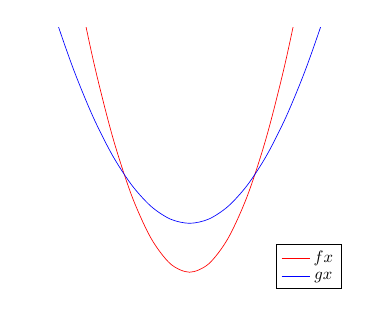
\begin{tikzpicture}[scale=0.6]
				\begin{axis}
					[ticks=none, axis x line=none, axis y line=none, xmin=-3.5, xmax=3.5, ymin=-0.5, ymax=5, axis line style={<->}, legend pos=south east]
					\addplot[smooth, red] {x^2};
					\addplot[smooth, blue] {0.5*x^2 + 1};
					
					\legend{$ \func{f}{x} $, $ \func{g}{x} $}
				\end{axis}
			\end{tikzpicture}
			\caption{Ilustrasi dua fungsi kuadrat $ \func{f}{x} $ dan $ \func{g}{x} $ yang berpotongan tepat di dua titik.}
		\end{figure}
		
		\par Selain berpotongan tepat pada dua titik, kedua fungsi $ f $ dan $ g $ juga memiliki kemungkinan untuk berpotongan tepat di satu titik. Seperti yang telah dijelaskan sebelumnya, jika $ \func{h}{x} $ merupakan fungsi linear takkonstan, maka persamaan $ \func{h}{x} = 0 $ akan memiliki tepat satu solusi. Akibatnya, fungsi $ f $ dan $ g $ akan berpotongan tepat di satu titik. Lain halnya jika kita menginginkan $ f $ dan $ g $ saling bersinggungan. Jika $ f $ dan $ g $ saling bersinggungan, maka $ \func{h}{x} $ haruslah berupa fungsi kuadrat. Selain itu, diskriminan persamaan kuadrat $ \func{h}{x} = 0 $ harus sama dengan nol.
		
		\par Kemudian muncul pertanyaan baru mengenai mengapa jika $ h $ fungsi linear takkonstan akan membuat dua fungsi $ f $ dan $ g $ berpotongan tepat di satu titik, tetapi ketika $ h $ fungsi kuadrat akan membuat dua fungsi $ f $ dan $ g $ bersinggungan. Hal ini berkaitan dengan fungsi $ \func{h}{x} $ itu sendiri. Ingat kembali bahwa $ \func{h}{x} = \func{f}{x} - \func{g}{x} $ atau dalam kata lain, $ \func{h}{x} $ ini sebenarnya merupakan selisih antara fungsi $ f $ dan $ g $. Ketika $ h $ merupakan fungsi linear takkonstan, maka pada suatu saat grafik fungsi $ h $ akan berpotongan dengan sumbu-$ x $ (yaitu ketika $ \func{h}{x} = 0 $) dan akan terjadi perubahan tanda. Berarti, terkadang $ \func{f}{x} < \func{g}{x} $ dan terkadang juga $ \func{f}{x} > \func{g}{x} $ pada suatu interval tertentu. Akibatnya, pastilah $ f $ dan $ g $ berpotongan tepat pada satu titik, yang persisnya adalah ketika $ \func{h}{x} = 0 $. Anda dapat menganggap kejadian ini seperti gunting yang menyilang. Ilustrasinya adalah sebagai berikut.
		\begin{figure}[H]
			\centering
			\begin{tikzpicture}[scale=0.6]
				\begin{axis}
					[ticks=none, axis x line=none, axis y line=none, xmin=-3.5, xmax=3.5, ymin=-1.5, ymax=3.5, axis line style={<->}, legend pos=south west]
					\addplot[smooth, red] {x^2 - 2*x};
					\addplot[smooth, blue] {x^2};
					
					\legend{$ \func{f}{x} $, $ \func{g}{x} $}
				\end{axis}
			\end{tikzpicture}
			\caption{Ilustrasi dua fungsi kuadrat $ \func{f}{x} $ dan $ \func{g}{x} $ yang berpotongan tepat di satu titik.}
		\end{figure}
		Lain halnya ketika $ h $ fungsi kuadrat. Ketika persamaan $ \func{h}{x} = 0 $ memiliki diskriminan nol, maka grafik fungsinya hanya akan menyinggung sumbu-$ x $. Akibatnya, selisih dari $ f $ dan $ g $ tidak akan pernah berubah tanda. Oleh karena itu, kedua fungsi tersebut hanya akan bersinggungan satu sama lain (yaitu ketika $ \func{h}{x} = 0 $). Ilustrasinya adalah sebagai berikut.
		\begin{figure}[H]
			\centering
			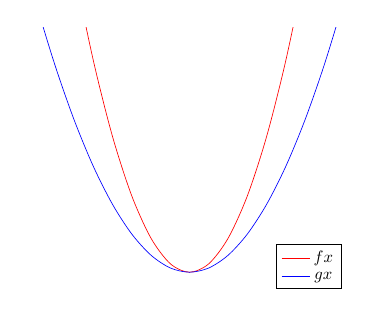
\begin{tikzpicture}[scale=0.6]
				\begin{axis}
					[ticks=none, axis x line=none, axis y line=none, xmin=-3.5, xmax=3.5, ymin=-0.5, ymax=5, axis line style={<->}, legend pos=south east]
					\addplot[smooth, red] {x^2};
					\addplot[smooth, blue] {0.5*x^2};
					
					\legend{$ \func{f}{x} $, $ \func{g}{x} $}
				\end{axis}
			\end{tikzpicture}
			\caption{Ilustrasi dua fungsi kuadrat $ \func{f}{x} $ dan $ \func{g}{x} $ yang saling bersinggungan.}
		\end{figure}
		
		\par Terakhir, agar kedua fungsi kuadrat $ f $ dan $ g $ tidak menyinggung maupun memotong satu sama lain, maka haruslah $ \func{h}{x} $ merupakan fungsi kuadrat atau fungsi konstan taknol. Jika $ \func{h}{x} $ berupa fungsi kuadrat, maka diskriminan persamaan $ \func{h}{x} = 0 $ haruslah kurang dari nol. Tetapi, jika $ \func{h}{x} $ berupa fungsi konstan taknol, maka hal tersebut sudah cukup untuk menjamin $ f $ dan $ g $ agar tidak menyinggung ataupun memotong satu sama lain. Selisih antara $ f $ dan $ g $ selalu konstan sehingga tidak akan memotong ataupun bersinggungan satu sama lain.
		\begin{figure}[H]
			\centering
			\begin{tikzpicture}[scale=0.6]
				\begin{axis}
					[ticks=none, axis x line=none, axis y line=none, xmin=-3.5, xmax=3.5, ymin=-0.5, ymax=5, axis line style={<->}, legend pos=south east]
					\addplot[smooth, red] {x^2 + 1};
					\addplot[smooth, blue] {0.3*x^2};
					
					\legend{$ \func{f}{x} $, $ \func{g}{x} $}
				\end{axis}
			\end{tikzpicture}
			\caption{Ilustrasi dua fungsi kuadrat $ \func{f}{x} $ dan $ \func{g}{x} $ yang tidak memotong ataupun bersinggungan satu sama lain karena $ \func{h}{x} $ berupa fungsi kuadrat dan diskriminannya kurang dari nol.}
		\end{figure}
		
		\par Jika fungsi $ \func{h}{x} $ konstan, atau dengan kata lain $ \func{h}{x} = k $ untuk suatu konstanta real $ k $, maka $ k $ tidak boleh nol. Tentunya jika $ k = 0 $, maka fungsi $ f $ dan $ g $ akan saling berhimpitan. Tetapi jika $ k \ne 0 $, maka seperti yang telah dijelaskan sebelumnya, selisih $ f $ dan $ g $ akan selalu konstan sehingga grafiknya tidak akan berpotongan maupun bersinggungan satu sama lain.
		
		\begin{explbox}
			Ilustrasikan dua fungsi kuadrat $ \func{f}{x} $ dan $ \func{g}{x} $ yang tidak memotong ataupun bersinggungan satu sama lain karena $ \func{h}{x} $ berupa fungsi konstan. Apa perbedaannya dengan ketika $ \func{h}{x} $ fungsi kuadrat berdiskriminan negatif?
		\end{explbox}
		
		\par Agar lebih jelas, kita akan mengerjakan beberapa contoh soal yang berkaitan dengan kedudukan fungsi kuadrat terhadap fungsi kuadrat lainnya.
		
		\begin{contoh}
			Tentukan kedudukan fungsi kuadrat $ \func{f}{x} = x^{2} + 3x - 1 $ dengan fungsi kuadrat $ \func{g}{x} = x^{2} + 1 $. Jika kedua fungsi tersebut berpotongan atau bersinggungan, tentukan titik potongnya atau titik singgungnya.
		\end{contoh}
		\begin{jawab}
			Perhatikan bahwa $ \func{f}{x} - \func{g}{x} = 3x - 2 $. Akibatnya, $ f $ dan $ g $ berpotongan tepat di satu titik, yaitu ketika $ 3x - 2 = 0 \iff x = 2/3 $. Oleh karena itu, titik potong $ f $ dan $ g $ adalah $ \left(2/3, \func{f}{2/3}\right) $ atau $ \left(2/3, \func{g}{2/3}\right) $.
			\par Karena $ \func{f}{2/3} = \func{g}{2/3} = \left(2/3\right)^{2} + 1 = 13/9 $, maka titik potongnya adalah $ \left(2/3, 13/9\right) $.
		\end{jawab}
		
		\begin{contoh}
			Tentukanlah syarat untuk $ m $ agar fungsi kuadrat $ \func{f}{x} = mx^{2} + 1 $ dan fungsi kuadrat $ \func{g}{x} = x^{2} + 2x $
			\begin{enumerate}
				\item saling berpotongan tepat di dua titik berbeda,
				\item saling berpotongan tepat di satu titik,
				\item saling bersinggungan,
				\item tidak bersinggungan atau berpotongan.
			\end{enumerate}
		\end{contoh}
		\begin{jawab}
			Ingat bahwa agar $ f $ merupakan fungsi kuadrat, maka $ m \ne 0 $. Syarat ini mutlak dipenuhi oleh setiap subsoal.
			\par Perhatikan bahwa dengan mengurangi $ \func{f}{x} $ dengan $ \func{g}{x} $ kita akan mendapatkan
			\[ \func{f}{x} - \func{g}{x} = \left(m - 1\right)x^{2} - 2x + 1. \]
			Fungsi yang didapatkan dari hasil pengurangan ini memiliki diskriminan $ \left(-2\right)^{2} - 4\left(m - 1\right)\left(1\right) = 8 - 4m $. Selanjutnya, misalkan $ \func{h}{x} = \func{f}{x} - \func{g}{x} $.
			\begin{enumerate}
				\item Agar kedua fungsi saling berpotongan di dua titik, maka $ \func{h}{x} $ haruslah merupakan fungsi kuadrat dengan diskriminan positif. Oleh karena itu, agar $ \func{h}{x} $ fungsi kuadrat, maka $ m - 1 \ne 0 \iff m \ne 1 $. Selain itu, haruslah $ 8 - 4m > 0 \iff m < 2 $.
				\par Jadi, agar kedua fungsi saling berpotongan di dua titik, haruslah $ m \in \left(-\infty, 2\right) \backslash \lrbr{0, 1} $.
				\item Agar kedua fungsi saling berpotongan tepat di satu titk, maka $ \func{h}{x} $ haruslah fungsi linear takkonstan sehingga haruslah $ m - 1 = 0 \iff m = 1 $.
				\item Agar kedua fungsi saling bersinggungan, maka $ \func{h}{x} $ haruslah merupakan fungsi kuadrat dengan diskriminan nol. Oleh karena itu, agar $ \func{h}{x} $ fungsi kuadrat, maka $ m - 1 \ne 0 \iff m \ne 1 $. Selain itu, haruslah $ 8 - 4m = 0 \iff m = 2 $.
				\par Jadi, agar kedua fungsi saling bersinggungan, haruslah $ m = 2 $.
				\item Agar kedua fungsi tidak bersinggungan atau berpotongan, maka $ \func{h}{x} $ haruslah merupakan fungsi kuadrat dengan diskriminan negatif atau fungsi konstan taknol. Jika kita lihat lebih lanjut, $ \func{h}{x} $ tidak mungkin fungsi konstan sehingga haruslah $ \func{h}{x} $ fungsi kuadrat. Oleh karena itu, agar $ \func{h}{x} $ fungsi kuadrat, maka $ m - 1 \ne 0 \iff m \ne 1 $. Selain itu, haruslah $ 8 - 4m < 0 \iff m > 2 $.
				\par Jadi, agar kedua fungsi tidak bersinggungan atau berpotongan, haruslah $ m \in \left(2, +\infty\right) $.
			\end{enumerate}
		\end{jawab}
		
		\begin{infobox}{Informasi}
			Jika Anda mengalami kesulitan untuk membayangkan bagaimana cara kerja soal ini, Anda dapat mencoba membuka laman daring https://www.desmos.com/calculator?lang=id. Kemudian buatlah grafik $ f $ dan $ g $ untuk contoh soal terakhir. Jangan lupa tambahkan slider $ m $ untuk melihat bagaimana kedudukan $ f $ terhadap $ g $ seiring berubahnya nilai $ m $.
		\end{infobox}
	
	\subsubsection{Kasus Khusus Ketika Tidak Ada Perpotongan Antara Dua Fungsi}
		
		Ketika tidak ada perpotongan antara fungsi kuadrat dengan fungsi lainnya, kita bisa membuat fungsi kuadrat tersebut selalu berada di atas fungsi lainnya ataupun selalu berada di bawah fungsi lainnya. Jika $ \func{f}{x} $ fungsi kuadrat dan $ \func{g}{x} $ fungsi linear, kita bisa membuat fungsi kuadrat $ f $ agar selalu berada di atas fungsi linear $ g $. Tentunya agar kondisi tersebut tercapai, haruslah $ \func{f}{x} > \func{g}{x} \iff \func{f}{x} - \func{g}{x} > 0 $ atau dengan kata lain, selisih antara $ f $ dan $ g $ harus positif. Akibatnya, $ \func{f}{x} - \func{g}{x} $ harus selalu berada di atas sumbu-$ x $ (karena harus positif) sehingga $ \func{f}{x} - \func{g}{x} $ harus definit positif. Dengan cara yang sama, agar fungsi kuadrat $ f $ selalu berada di bawah fungsi linear $ g $, maka $ \func{f}{x} - \func{g}{x} $ harus definit negatif. Tentunya ketika $ f $ fungsi kuadrat dan $ g $ fungsi linear, maka fungsi $ \func{f}{x} - \func{g}{x} $ akan terjamin merupakan fungsi kuadrat sehingga syarat-syarat definitnya sama dengan syarat-syarat yang telah kita pelajari pada bagian sebelumnya.
		
		\par Lain halnya ketika $ \func{f}{x} $ dan $ \func{g}{x} $ keduanya fungsi kuadrat. Langkah-langkahnya sama dengan paragraf sebelumnya ketika $ \func{f}{x} - \func{g}{x} $ merupakan fungsi kuadrat. Tetapi, jika $ \func{f}{x} - \func{g}{x} $ bukan merupakan fungsi kuadrat, melainkan fungsi linear takkonstan, maka kita tidak akan bisa membuat $ f $ selalu berada di atas $ g $ atau sebaliknya. Hal ini dikarenakan fungsi linear takkonstan pasti akan selalu berpotongan dengan sumbu-$ x $ yang membuat $ \func{f}{x} - \func{g}{x} $ mustahil selalu berada di atas sumbu-$ x $ maupun dibawahnya.
		
		\begin{explbox}
			Bagaimana jika $ \func{f}{x} - \func{g}{x} $ fungsi konstan (baik nol maupun taknol)?
		\end{explbox}
		
		\par Agar lebih jelas, kita akan mengerjakan beberapa contoh soal yang berkaitan dengan kasus khusus ketika tidak ada perpotongan antara dua fungsi ini.
		
		\begin{contoh}
			Tentukanlah syarat untuk $ m $ agar grafik fungsi $ \func{f}{x} = mx^{2} - 2mx + m $ seluruhnya berada di atas fungsi $ \func{g}{x} = 2x - 3 $.
		\end{contoh}
		\begin{jawab}
			Pada soal ini tidak disebutkan secara eksplisit jika $ f $ merupakan 'fungsi kuadrat', tetapi hanya 'fungsi'. Berarti syarat $ m \ne 0 $ tidak diperlukan.
			\par Agar grafik fungsi $ f $ seluruhnya berada di atas fungsi $ g $, maka haruslah
			\[ \func{f}{x} - \func{g}{x} = mx^{2} - \left(2m + 2\right)x + m + 3 > 0. \]
			Perhatikan bahwa $ \func{f}{x} - \func{g}{x} $ memiliki kemungkinan untuk menjadi fungsi linear (ketika $ m = 0 $). Padahal $ \func{f}{x} - \func{g}{x} $ harus merupakan fungsi kuadrat yang memaksa kita untuk memerlukan syarat $ m \ne 0 $. Selain itu, fungsi kuadrat $ \func{f}{x} - \func{g}{x} $ harus definit positif. Akibatnya $ m > 0 $ dan
			\[ \left(-\left(2m + 2\right)\right)^{2} - 4m\left(m\right) = 8m + 4 < 0 \iff m < -\frac{1}{2}. \]
			Tetapi, perpotongan ketiga syarat tersebut merupakan himpunan kosong.
			\par Jadi, tidak ada nilai $ m $ sedemikian sehingga grafik fungsi $ f $ seluruhnya berada di atas fungsi $ g $.
		\end{jawab}
		
		\begin{contoh}
			Tentukanlah syarat untuk $ m $ agar grafik fungsi $ \func{f}{x} = x^{2} - 3 $ seluruhnya berada di bawah fungsi $ \func{g}{x} = mx^{2} + 2x $.
		\end{contoh}
		\begin{jawab}
			latihan.
		\end{jawab}
	
\subsection{Titik Tetap dan Titik Invarian Fungsi Kuadrat}
	
	Dalam fungsi kuadrat, bahkan juga fungsi secara umum, terdapat istilah titik tetap dan titik invarian. Titik tetap suatu fungsi didefinisikan sebagai suatu elemen pada domain fungsi yang dipetakan ke dirinya sendiri oleh fungsi tersebut. Dengan kata lain, titik $ c $ adalah titik tetap fungsi $ \func{f}{x} $ jika dan hanya jika $ \func{f}{c} = c $. Sebagai contoh, pada fungsi kuadrat $ \func{f}{x} = x^{2} - 3x + 4 $, titik $ x = 2 $ merupakan titik tetap fungsi $ f $ karena $ \func{f}{2} = 2^{2} - 3\left(2\right) + 4 = 2 $. Secara geometris, titik tetap adalah titik dimana suatu grafik fungsi $ f $ berpotongan/bersinggungan dengan garis $ y = x $. Berdasarkan bagian sebelumnya, fungsi kuadrat hanya dapat berpotongan dengan fungsi linear paling banyak di dua titik berbeda. Oleh karena itu, fungsi kuadrat akan memiliki paling banyak dua titik tetap. Berikut merupakan ilustrasinya.
	\begin{figure}[H]
		\centering
		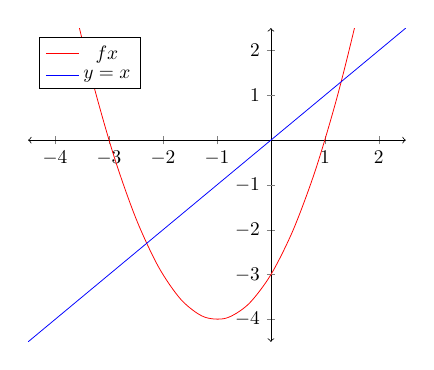
\begin{tikzpicture}[scale=0.7]
			\begin{axis}
				[axis x line=center, axis y line=center, extra y ticks={-3, -1, 1}, extra y tick labels={$ -3 $, $ -1 $, 1}, ymin=-4.5, ymax=2.5, xmin=-4.5, xmax=2.5, axis line style={<->}, legend pos=north west]
				\addplot[smooth, red] {x^2 + 2*x - 3};
				\addplot[smooth, blue] {x};
				
				\legend{$ \func{f}{x} $, $ y = x $}
			\end{axis}
		\end{tikzpicture}
		\caption{Ilustrasi fungsi kuadrat $ \func{f}{x} $ yang memiliki dua titik tetap, yaitu titik-titik yang berpotongan dengan garis $ y = x $.}
	\end{figure}
	
	\par Secara umum, jika $ \func{f}{x} $ adalah fungsi kuadrat umum \ref{eq:222}, maka titik-titik tetapnya memenuhi persamaan
	\[ ax^{2} + bx + c = x \iff ax^{2} + \left(b - 1\right)x + c = 0 \]
	sehingga dengan menggunakan rumus kuadratik, titik-titik tetap $ x_{\fixed_{1, 2}} $ fungsi kuadrat $ f $ adalah
	\begin{equation} \label{eq:229}
		x_{\fixed_{1, 2}} = \frac{-b + 1 \pm \sqrt{\left(b - 1\right)^{2} - 4ac}}{2a}.
	\end{equation}
	Disini, titik-titik tetap biasa dinotasikan dengan $ x_{\fixed} $ dengan $ \fixed $ disini berarti \textit{fixed} (tetap) dan bukan merujuk kepada fungsi $ f $.
	
	\par Selain memiliki titik tetap, fungsi kuadrat juga memiliki titik invarian. Beberapa matematikawan menyebut titik invarian ini sebagai titik tetap. Tetapi, karena titik tetap sudah memiliki definisinya tersendiri dalam matematika, maka dalam buku ini dituliskan sebagai \textit{titik invarian}. Titik invarian fungsi kuadrat didefinisikan sebagai titik-titik yang selalu dilalui oleh fungsi kuadrat $ f $ meskipun beberapa koefisien-koefisiennya berubah. Sebagai contoh, titik invarian fungsi kuadrat $ \func{f}{x} = x^{2} $ memiliki titik invarian $ \left(0, 0\right) $. Hal ini disebabkan ketika koefisien $ x^{2} $ pada fungsi $ f $ tersebut diubah-ubah, titik $ \left(0, 0\right) $ ini akan tetap dilalui oleh fungsi $ f $ yang termodifikasi tersebut. Berikut merupakan ilustrasinya.
	\begin{figure}[H]
		\centering
		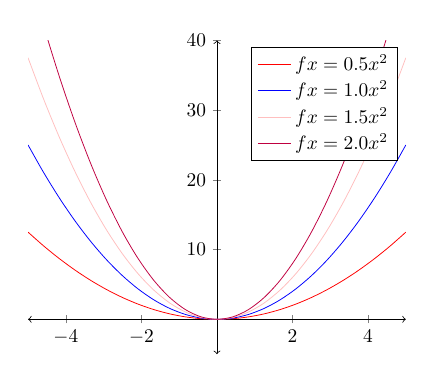
\begin{tikzpicture}[scale=0.7]
			\begin{axis}
				[axis x line=center, axis y line=center, ymin=-5, ymax=40, axis line style={<->}]
				\addplot[smooth, red] {0.5 * x^2};
				\addplot[smooth, blue] {x^2};
				\addplot[smooth, pink] {1.5 * x^2};
				\addplot[smooth, purple] {2 * x^2};
				
				\legend{$ \func{f}{x} = 0.5x^2 $, $ \func{f}{x} = 1.0x^2 $, $ \func{f}{x} = 1.5x^2 $, $ \func{f}{x} = 2.0x^2 $};
			\end{axis}
		\end{tikzpicture}
		\caption{Grafik fungsi kuadrat $ \func{f}{x} $ ketika koefisien $ x^{2} $-nya berubah. Perhatikan bahwa titik $ \left(0, 0\right) $ selalu dilalui oleh fungsi yang termodifikasi.}
	\end{figure}
	
	\par Terdapat dua cara untuk mencari titik-titik invarian fungsi kuadrat. Untuk mendemonstrasikannya, kita akan mengerjakan contoh soal berikut.
	
	\begin{contoh}
		Untuk setiap bilangan real $ m $, tentukanlah titik-titik invarian fungsi kuadrat
		\[ \func{f}{x} = \left(m - 3\right)x^{2} - \left(3m - 9\right)x + 30 - 10m. \]
	\end{contoh}
	\begin{jawab}
		Cara pertama adalah dengan menguraikan fungsi kuadrat $ \func{f}{x} $, lalu memfaktorkan suku-suku yang mengandung variabel $ m $. Untuk itu, pertama-tama kita tulis ulang fungsi $ f $ sebagai
		\begin{align*}
			\func{f}{x} &= \left(m - 3\right)x^{2} - \left(3m - 9\right)x + 30 - 10m \\
			&= mx^{2} - 3x^{2} - 3mx + 9x + 30 - 10m \\
			&= m\left(x^{2} - 3x - 10\right) - 3x^{2} + 9x + 30 \\
			&= m\left(x + 2\right)\left(x - 5\right) - 3x^{2} + 9x + 30
		\end{align*}
		Perhatikan bahwa ketika $ x = -2 $, ekspresi $ m\left(x + 2\right)\left(x - 5\right) $ akan selalu bernilai nol untuk setiap $ m \in \mathbb{R} $. Artinya, titik $ \left(-2, \func{f}{-2}\right) $ akan selalu dilalui oleh fungsi $ f $ berapapun nilai $ m $-nya. Selain itu, titik $ \left(5, \func{f}{5}\right) $ juga akan selalu dilalui oleh fungsi $ f $ berapapun nilai $ m $-nya. Inilah alasan mengapa kita menguraikan fungsi $ f $, kemudian memfaktorkan keluar $ m $. Hal ini akan mempermudah kita untuk mencari nilai $ x $ agar ekspresi yang mengandung $ m $ ini akan selalu bernilai nol.
		\par Dari persamaan terakhir, $ \func{f}{-2} = 0 - 3\left(-2\right)^{2} + 9\left(-2\right) + 30 = 0 $ dan $ \func{f}{5} = 0 - 3\left(5\right)^{2} + 9\left(5\right) + 30 = 0 $ sehingga titik-titik invarian fungsi $ f $ adalah $ \left(-2, 0\right) $ dan $ \left(5, 0\right) $.
		\begin{figure}[H]
			\centering
			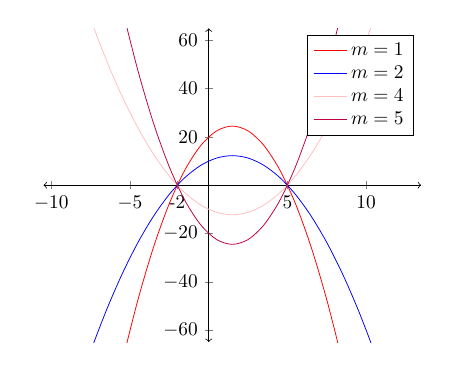
\begin{tikzpicture}[scale=0.7]
				\begin{axis}
					[axis x line=center, axis y line=center, extra x ticks={-2}, extra x tick labels={-2}, xmin=-10.5, xmax=13.5, ymin=-65, ymax=65, axis line style={<->}]
					\addplot[smooth, red, domain=-10.5:13.5] {-2*x^2 + 6*x + 20};
					\addplot[smooth, blue, domain=-10.5:13.5] {-x^2 + 3*x + 10};
					\addplot[smooth, pink, domain=-10.5:13.5] {x^2 - 3*x - 10};
					\addplot[smooth, purple, domain=-10.5:13.5] {2*x^2 - 6*x - 20};
					
					\legend{$ m = 1 $, $ m = 2 $, $ m = 4 $, $ m = 5 $};
				\end{axis}
			\end{tikzpicture}
			\caption{Grafik fungsi kuadrat $ \func{f}{x} $ untuk beberapa nilai $ m $. Perhatikan bahwa titik $ \left(-2, 0\right) $ dan $ \left(5, 0\right) $ selalu dilalui oleh grafik fungsi $ \func{f}{x} $.}
		\end{figure}
		Selain dengan penguraian, terdapat juga cara kedua untuk mencari titik-titik invarian fungsi kuadrat. Cara kedua ini adalah dengan memisalkan titik-titik invarian ini sebagai $ \left(p, q\right) $, kemudian mensubstitusi beberapa nilai $ m $. Untuk itu, pertama-tama kita misalkan titik-titik invarian fungsi $ f $ sebagai titik $ \left(p, q\right) $. Karenanya, untuk setiap bilangan real $ m $, titik $ \left(p, q\right) $ ini pasti akan selalu dilalui oleh fungsi $ f $.
		\par Ambil $ m = 3 $, maka $ \func{f}{x} = \left(3 - 3\right)x^{2} - \left(3\left(3\right) - 9\right)x + 30 - 10\left(3\right) = 0 $. Akibatnya $ \func{f}{x} \equiv 0 $ sehingga $ q = 0 $. Selanjutnya ambil $ m = 0 $, maka $ \func{f}{x} = \left(0 - 3\right)x^{2} - \left(3\left(0\right) - 9\right)x + 30 - 10\left(0\right) = -3x^{2} + 9x + 30 $. Karena $ \left(p, q\right) $ selalu dilalui oleh $ f $, maka $ \left(p, q\right) $ memenuhi $ q = -3p^{2} + 9p + 30 $. Mengingat $ q = 0 $, maka
		\[ 0 = -3p^{2} + 9p + 30 \iff 0 = p^{2} - 3p - 10 \iff \left(p + 2\right)\left(p - 5\right) = 0. \]
		Jadi, titik-titik invarian fungsi $ f $ adalah $ \left(-2, 0\right) $ dan $ \left(5, 0\right) $.
	\end{jawab}
	
	\par Pada bagian-bagian sebelumnya, kita tahu bahwa kita bisa mengonstruksi fungsi kuadrat dari tiga titik yang dilaluinya. Dari tiga titik ini, kita akan bisa membentuk fungsi kuadrat yang unik karena sistem persamaan linear yang dibentuk oleh ketiga titik tersebut akan menghasilkan koefisien-koefisien $ a $, $ b $, dan $ c $ yang unik. Artinya, ketiga titik tersebut hanya akan menghasilkan satu dan hanya satu fungsi kuadrat. Tidak akan ada lagi fungsi kuadrat lain yang dilalui oleh ketiga titik tersebut. Akibatnya, fungsi kuadrat $ f $ hanya memiliki titik invarian paling banyak dua.
	
	\begin{explbox}
		Apakah mungkin ada suatu fungsi kuadrat yang tidak memiliki titik invarian? Jika ada, berikan contohnya.
	\end{explbox}
	
\subsection{Penerapan Fungsi Kuadrat dalam Kehidupan Sehari-hari}
	
	Fungsi kuadrat memiliki penerapan dalam kehidupan sehari-hari. Biasanya fungsi kuadrat digunakan untuk permasalahan optimisasi, seperti memaksimalkan luas pekarangan rumah yang dipagari atau meminimumkan biaya pemagarannya. Tentunya permasalahan optimisasi ini cenderung diselesaikan dengan menggunakan kalkulus karena menyediakan alat-alat yang lebih lengkap dan dapat digunakan untuk berbagai macam fungsi, tidak terbatas pada fungsi kuadrat saja.
	
	\par Proses optimisasi menggunakan konsep fungsi kuadrat ini tentunya memerlukan pengetahuan yang cukup mengenai titik baliknya. Dari titik balik ini, akan didapatkan nilai yang telah teroptimisasi. Untuk lebih memahaminya, kita akan mengerjakan beberapa contoh berikut.
	
	\begin{contoh}
		Sebidang tanah terletak di belakang sisi suatu gudang. Tanah ini akan dipagari dengan kawat untuk membuat kandang ayam yang berbentuk persegi panjang. Kandang ayam tersebut dibuat menempel dengan dinding belakang gudang untuk meminimalkan penggunaan kawat. Jika kawat yang tersedia adalah $ 400 \punit{m} $, tentukan luas maksimum kandang ayam yang dapat dibuat. 
	\end{contoh}
	\begin{jawab}
		Dari deskripsi pada soal, kita hanya akan memagari kandang ayam tersebut pada tiga sisi selain sisi yang menyentuh (berhimpitan) dengan dinding belakang gudang. Misalkan panjang dan lebar kandang ayam tersebut berturut-turut adalah $ p $ dan $ \ell $. Ilustrasinya adalah sebagai berikut.
		\begin{figure}[H]
			\centering
			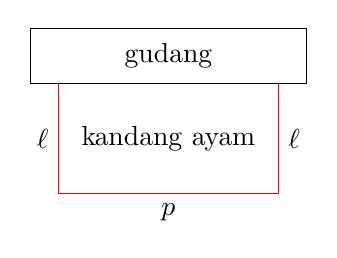
\begin{tikzpicture}[scale=0.7]
				\coordinate (A) at (0, 0);
				\coordinate (B) at (5, 0);
				\coordinate (C) at (5, 1);
				\coordinate (D) at (0, 1);
				\coordinate (X) at (0.5, -2);
				\coordinate (Y) at (4.5, -2);
				\coordinate (Z) at (4.5, 0);
				\coordinate (W) at (0.5, 0);
				
				\draw (A) -- (B) -- (C) -- (D) -- cycle;
				\draw[color=red] (W) -- (X) -- (Y) -- (Z);
				
				\path (W) -- (X) node[midway, left] {$ \ell $};
				\path (X) -- (Y) node[midway, below] {$ p $};
				\path (Y) -- (Z) node[midway, right] {$ \ell $};
				
				\node at (barycentric cs:A=1,B=1,C=1,D=1) {gudang};
				\node at (barycentric cs:W=1,X=1,Y=1,Z=1) {kandang ayam};
			\end{tikzpicture}
			\caption{Ilustrasi permasalahan pada soal. Perhatikan bahwa garis merah berarti sisi-sisi yang akan dipagari.}
		\end{figure}
		Karena kawat yang tersedia untuk memagari kandang ayam adalah $ 400 \punit{m} $, maka $ p + 2\ell = 400 \iff p = 400 - 2\ell $ dengan $ 0 < p < 400 $ dan $ 0 < \ell < 200 $ (mengapa?). Perhatikan bahwa luas kandang ayam $ L $ memenuhi $ L = pl = \left(400 - 2\ell\right)\ell = -2\ell^{2} + 400\ell $. Karena grafik $ L $ terbuka ke bawah, maka $ L $ akan mencapai nilai maksimumnya ketika $ \ell = -\dfrac{400}{2\left(-2\right)} = 100 $. Akibatnya, $ p = 400 - 2\left(100\right) = 200 $. Oleh karena itu, agar luasnya maksimum, haruslah $ p = 200 \punit{m} $ dan $ \ell = 100 \punit{m} $.
		\par Jadi, luas maksimum kandang ayam adalah $ L_{\mathrm{max}} = 200\left(100\right) = 20000 \punit{m^{2}} $.
	\end{jawab}
	
	\begin{explbox}
		Coba cari tahu mengenai ketaksamaan AM-GM. Gunakan ketaksamaan AM-GM ini untuk menentukan luas kandang maksimum dengan cepat.
	\end{explbox}
	
	\begin{contoh}
		Pemerintah daerah Kota Bontang berencana akan membuat rumah tahanan (rutan). Rutan tersebut terdiri dari 5 blok dan setiap bloknya terdiri dari tiga sel penjara yang berdampingan. Tepi kanan dan tepi kiri setiap blok dibatasi oleh tembok, begitu juga dengan bagian belakang bloknya. Pemerintah menginginkan setiap sel penjara memiliki luas yang sama. Jika jeruji besi yang tersedia ada sepanjang $ 2000 \punit{m} $ dan setiap meternya pada setiap sel penjara diperlukan sebanyak $ 10 \punit{m} $ jeruji besi, tentukan luas maksimum setiap sel penjara.
	\end{contoh}
	\begin{jawab}
		Dari deskripsi pada soal, misalkan panjang dan lebar setiap sel penjara berturut-turut adalah $ p $ dan $ \ell $. Ilustrasi setiap bloknya adalah sebagai berikut.
		\begin{figure}[H]
			\centering
			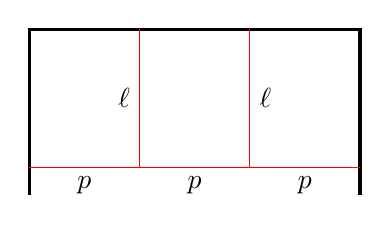
\begin{tikzpicture}[scale=0.7]
				\coordinate (A) at (0, 0);
				\coordinate (B) at (6, 0);
				\coordinate (C) at (6, 3);
				\coordinate (D) at (0, 3);
				\coordinate (P) at (0, 0.5);
				\coordinate (Q) at (6, 0.5);
				\coordinate (R) at (2, 3);
				\coordinate (S) at (4, 3);
				\coordinate (T) at (2, 0.5);
				\coordinate (U) at (4, 0.5);
				
				\draw[very thick] (A) -- (D) -- (C) -- (B);
				\draw[color=red] (P) -- (Q);
				\draw[color=red] (R) -- (T);
				\draw[color=red] (S) -- (U);
				
				\path (R) -- (T) node[midway, left] {$ \ell $};
				\path (S) -- (U) node[midway, right] {$ \ell $};
				\path (P) -- (T) node[midway, below] {$ p $};
				\path (T) -- (U) node[midway, below] {$ p $};
				\path (U) -- (Q) node[midway, below] {$ p $};
			\end{tikzpicture}
			\caption{Ilustrasi permasalahan pada soal. Perhatikan bahwa garis merah berarti sisi-sisi yang akan diberi jeruji besi.}
		\end{figure}
		Dari ilustrasi tersebut, panjang total sisi sel penjara yang akan diberi jeruji besi adalah $ 3p + 2\ell $. Karena terdapat 5 blok pada rutan tersebut, maka setiap bloknya memerlukan $ 2000/5 = 400 \punit{m} $ jeruji besi. Lebih jauh, karena per meter dari sisi penjara yang akan diberi jeruji besi ini membutuhkan $ 10 \punit{m} $ jeruji besi, maka total jeruji besi per bloknya adalah $ 10\left(3p + 2\ell\right) $. Akibatnya,
		\[ 10\left(3p + 2\ell\right) = 400 \iff 3p + 2\ell = 40 \iff \ell = 20 - \frac{3}{2}p \]
		dengan $ 0 < p < 40/3 $ dan $ 0 < \ell < 20 $ (mengapa?). Selanjutnya, perhatikan bahwa luas $ L $ setiap sel penjara adalah
		\[ L = p\ell = p\left(20 - \frac{3}{2}p\right) = -\frac{3}{2}p^{2} + 20p. \]
		Karena grafik $ L $ terbuka ke bawah, maka $ L $ akan mencapai nilai maksimumnya ketika $ p = -\dfrac{20}{2\left(-3/2\right)} = \dfrac{20}{3} $. Akibatnya, $ \ell = 20 - \dfrac{3}{2}\left(\dfrac{20}{3}\right) = 10 $. Oleh karena itu, agar luasnya maksimum, haruslah $ p = \dfrac{20}{3} \punit{m} $ dan $ \ell = 10 \punit{m} $.
		\par Jadi, luas maksimum setiap sel penjara adalah $ L_{\mathrm{max}} = \dfrac{20}{3}\left(10\right) = \dfrac{200}{3} \approx 66,6 \punit{m^{2}} $.
	\end{jawab}
	
\subsection{Fungsi Kuadrat Umum*}
	
	Pada subbab ini, kita telah mempelajari fungsi kuadrat secara mendetail. Tetapi, fungsi kuadrat yang kita pelajari pada subbab ini ternyata hanya merupakan kasus khusus. Fungsi kuadrat yang telah kita pelajari ini merupakan fungsi kuadrat satu variabel atau biasa disebut juga sebagai fungsi kuadrat univariat.
	
	\par Fungsi kuadrat juga bisa memiliki lebih dari satu variabel yang biasa disebut sebagai fungsi kuadrat multivariat. Artinya, fungsi kuadrat tersebut memerlukan dua input atau lebih. Akibatnya, domainnya bukan bilangan real, tetapi tupel bilangan real. Salah satu fungsi kuadrat dengan variabel lebih dari satu adalah fungsi kuadrat bivariat, yaitu fungsi kuadrat dua variabel. Bentuk umum fungsi kuadrat bivariat adalah
	\begin{equation} \label{eq:230}
		\func{f}{x, y} = ax^{2} + by^{2} + cxy + dx + ey + f
	\end{equation}
	dengan $ a, b, c, d, e, f $ adalah koefisien-koefisien dari fungsi tersebut. Anda akan mempelajari fungsi kuadrat dua variabel ini pada mata kuliah geometri analitik untuk studi yang lebih mendalam mengenai irisan kerucut.
	
	\begin{explbox}
		Carilah informasi mengenai fungsi kuadrat tiga variabel atau lebih. Bagaimana bentuk umum fungsi kuadrat dengan $ n $ variabel?
	\end{explbox}

\subsection{Contoh Soal HOTS}
	
	Subbab ini tentunya harus diakhiri dengan memberikan contoh-contoh soal HOTS agar pembaca dapat lebih kritis dan lebih menguasai lagi materi-materi yang telah diberikan pada subbab ini. Pembaca diharapkan dapat mencoba untuk mengerjakan contoh-contoh ini terlebih dahulu sebelum membaca solusinya.
	
	\begin{contoh}[Baltic Way 2011 P5]
		Misalkan $ f : \mathbb{R} \to \mathbb{R} $ fungsi yang memenuhi $ \func{f}{\func{f}{x}} = x^{2} - x + 1 $ untuk setiap bilangan real $ x $. Hitunglah nilai dari $ \func{f}{0} $.
	\end{contoh}
	\begin{jawab}
		Misalkan $ \func{f}{0} = a $ dan $ \func{f}{1} = b $. Maka $ \func{f}{\func{f}{0}} = \func{f}{a} $. Tetapi dari soal kita tahu bahwa $ \func{f}{\func{f}{0}} = 0^{2} - 0 + 1 = 1 $. Oleh karena itu $ \func{f}{a} = 1 $.
		\par Perhatikan juga bahwa $ \func{f}{\func{f}{1}} = b $. Tetapi dari soal kita juga tahu bahwa $ \func{f}{\func{f}{1}} = 1^{2} - 1 + 1 = 1 $. Oleh karena itu $ \func{f}{b} = 1 $.
		\par Karena $ \func{f}{a} = 1 $, maka $ \func{f}{\func{f}{a}} = \func{f}{1} $. Tetapi dari soal kita tahu bahwa $ \func{f}{\func{f}{a}} = a^{2} - a + 1 $. Oleh karena itu $ a^{2} - a + 1 = b $.
		\par Karena $ \func{f}{b} = 1 $, maka $ \func{f}{\func{f}{b}} = \func{f}{1} = b $. Tetapi dari soal kita juga tahu bahwa $ \func{f}{\func{f}{b}} = b^{2} - b + 1 $. Oleh karena itu
		\[ b^{2} - b + 1 = b \iff b^{2} - 2b + 1 = 0 \iff \left(b - 1\right)^{2} = 0 \iff b = 1. \]
		Berarti $ a^{2} - a + 1 = 1 \iff a\left(a - 1\right) = 0 $. Jika $ a = 0 $, maka $ \func{f}{\func{f}{0}} = 0 $ yang mana hal tersebut tidak mungkin. Jadi $ a = 1 $ atau dengan kata lain $ \func{f}{0} = 1 $ dan kita selesai.
	\end{jawab}
	
	\begin{contoh}[OSN 2020 P2]
		Diberikan fungsi kuadrat $ \func{P}{x} = ax^{2} + bx + c $ dimana $ a $, $ b $, dan $ c $ bilangan real. Jika
		\[ \func{P}{a} = bc, \quad \func{P}{b} = ca, \quad \mbox{dan} \quad \func{P}{c} = ab, \]
		buktikan bahwa
		\[ \left(a - b\right)\left(b - c\right)\left(c - a\right)\left(a + b + c\right) = 0. \]
	\end{contoh}
	\begin{jawab}
		Karena $ \func{P}{a} = bc $, $ \func{P}{b} = ca $, dan $ \func{P}{c} = ab $, maka kita punyai sistem persamaan
		\[
			\begin{cases}
				\begin{aligned}
					a^{3} + ab + c &= bc \\
					ab^{2} + b^{2} + c &= ca \\
					ac^{2} + bc + c &= ab
				\end{aligned}
			\end{cases}
		\]
		Mengurangi persamaan (2) dengan persamaan (3), kita akan mendapatkan
		\begin{alignat*}{2}
			&\qquad& ab^{2} + b^{2} - ac^{2} - bc &= ca - ab \\
			\iff&& a\left(b^{2} - c^{2}\right) + b\left(b - c\right) &= a\left(c - b\right) \\
			\iff&& a\left(b + c\right)\left(b - c\right) + b\left(b - c\right) + a\left(b - c\right) &= 0 \\
			\iff&& \left(b - c\right)\left(ab + ac + a + b\right) &= 0
		\end{alignat*}
		Jika $ b - c = 0 $, maka kita selesai. Oleh karena itu, selanjutnya misalkan $ ab + ac + a + b = 0 $.
		\par Perhatikan juga bahwa jika kita mengurangi persamaan (1) dengan persamaan (2), maka kita akan mendapatkan
		\begin{alignat*}{2}
			&\qquad& a^{3} + ab - ab^{2} - b^{2} &= bc - ca \\
			\iff&& a\left(a^{2} - b^{2}\right) + b\left(a - b\right) &= c\left(b - a\right) \\
			\iff&& a\left(a + b\right)\left(a - b\right) + b\left(a - b\right) + c\left(a - b\right) &= 0 \\
			\iff&& \left(a - b\right)\left(a^{2} + ab + b + c\right) &= 0
		\end{alignat*}
		Jika $ a - b = 0 $, maka kita selesai. Oleh karena itu, selanjutnya misalkan $ a^{2} + ab + b + c = 0 $.
		\par Sampai saat ini, kita punyai $ ab + ac + a + b = 0 $ dan $ a^{2} + ab + b + c = 0 $. Mengurangi kedua persamaan tersebut akan didapatkan
		\[ ac + c - a^{2} - c = 0 \iff a\left(c - a\right) - \left(c - a\right) = 0 \iff \left(c - a\right)\left(a - 1\right) = 0. \]
		Tentunya jika $ c - a = 0 $, maka kita selesai. Oleh karena itu, selanjutnya misalkan $ a = 1 $. Akibatnya, mensubstitusikannya pada persamaan (2) kita akan mendapatkan $ b = 0 $ (cek!). Mensubstitusikan nilai $ a $ dan $ b $ ini ke persamaan (1), kita juga akan mendapatkan $ c = -1 $ (cek!). Setelah solusi ini di substitusikan ke persamaan (3), ternyata solusi ini juga memenuhi sehingga solusi ini valid (cek!). Berarti $ a + b + c = 1 + 0 - 1 = 0 $.
		\par Jadi terbukti bahwa $ \left(a - b\right)\left(b - c\right)\left(c - a\right)\left(a + b + c\right) = 0 $. \hfill $ \square $
	\end{jawab}
	
\newpage

\subsection{Latihan Soal 2.2}
	
	\subsubsection{Bagian Pertama}
		
		\begin{enumerate}[topsep=0pt]
			\item Tentukan apakah masing-masing fungsi berikut merupakan fungsi kuadrat atau tidak. Jika termasuk fungsi kuadrat, tentukan koefisien-koefisiennya.
			\begin{multcols}
				\begin{enumerate}
					\item $ \func{f}{x} = x^{2} + 1 $
					\item $ \func{g}{x} = \sqrt{x} $
					\item $ \func{f}{x} = ax^{2} + by - c $
					\item $ \func{h}{x} = xy^{2} + 2x - 1 $
					\item $ \func{u}{\gamma} = \gamma^{4} + 2\gamma^{2} + 8x $
				\end{enumerate}
			\end{multcols}
			\item Diberikan fungsi kuadrat $ \func{f}{x} = 3x^{2} + \alpha x + 7 $. Jika $ \func{f}{3} = 1 $, tentukan nilai dari $ a $.
			\item Jika $ \func{f}{2x - 1} = x^{2} - 5x - 1 $, tentukanlah $ \func{f}{x} $.
			\item Jika $ \func{f}{x} = -3x^{2} - x + 10 $, tentukanlah $ \func{f}{x + 1} $.
			\item Titik $ \left(-4, a\right) $, $ \left(0, 1\right) $, dan $ \left(-3, b\right) $ dilalui oleh grafik fungsi kuadrat $ \func{s}{x} = -x^{2} - 8x + c $. Tentukan nilai dari $ a + b - c $.
			\item Titik $ \left(-3, -25\right) $ dan $ \left(1, 3\right) $ dilalui oleh grafik fungsi $ \func{f}{x} = ax^{2} + bx + 2 $. Tentukan nilai dari $ ab^{2} $.
			\item Buat sketsa grafik fungsi $ \func{f}{x} = ax^{2} + bx + c $ dengan syarat
			\begin{enumerate}
				\item $ a > 0 $, $ b > 0 $, $ c < 0 $, dan $ b^{2} - 4ac > 0 $
				\item $ a < 0 $, $ b > 0 $, $ c < 0 $, dan $ b^{2} - 4ac > 0 $
				\item $ a > 0 $, $ b = 0 $, $ c < 0 $, dan $ b^{2} - 4ac < 0 $
				\item $ a > 0 $, $ b > 0 $, $ c < 0 $, dan $ b^{2} - 4ac < 0 $
				\item $ a > 0 $, $ b < 0 $, $ c = 0 $, dan $ b^{2} - 4ac > 0 $
				\item $ a < 0 $, $ b < 0 $, $ c < 0 $, dan $ b^{2} - 4ac = 0 $
				\item $ a < 0 $, $ b < 0 $, $ c < 0 $, dan $ b^{2} - 4ac < 0 $
				\item $ a > 0 $, $ b > 0 $, $ c > 0 $, dan $ b^{2} - 4ac > 0 $
				\item $ a > 0 $, $ b = 0 $, $ c = 0 $, dan $ b^{2} - 4ac = 0 $
			\end{enumerate}
			\item Untuk masing-masing fungsi kuadrat berikut, tentukan kecekungannya, tanda sumbu simetri, titik potong dengan sumbu-$ y $, dan banyaknya perpotongan dengan sumbu-$ x $.
			\begin{multcols}
				\begin{enumerate}
					\item $ \func{f}{x} = -x^{2} + 2x - 11 $
					\item $ \func{f}{x} = -3x^{2} + 9x - 10 $
					\item $ \func{f}{x} = x^{2} + x + 1 $
					\item $ \func{f}{x} = -\dfrac{1}{2}x^{2} - 2x + 3 $
					\item $ \func{f}{x} = \dfrac{3}{5}x^{2} + \dfrac{5}{3}x + \dfrac{7}{2} $
					\item $ \func{f}{x} = 5x^{2} - 10x + 1 $
					\item $ \func{f}{x} = -x^{2} - x $
					\item $ \func{f}{x} = x^{2} + 1 $
				\end{enumerate}
			\end{multcols}
			\item Tentukan tanda untuk $ a $, $ b $, $ c $, dan $ b^{2} - 4ac $ untuk masing-masing sketsa grafik fungsi kuadrat berikut.
			\begin{multcols}
				\begin{enumerate}
					\item	\begin{tikzpicture}[baseline={($ (current bounding box.north)-(0, 1.6ex) $)}, scale=0.7]
								\begin{axis}
									[ticks=none, axis x line=center, axis y line=center, xmin=-4.5, xmax=4.5, ymin=-4.5, ymax=4.5, axis line style={<->}, legend pos=north west]
									\addplot[smooth, red] {-x^2 + 2*x + 1};
									
									\legend{$ \func{f}{x} = ax^{2} + bx + c $}
								\end{axis}
							\end{tikzpicture}
					\item	\begin{tikzpicture}[baseline={($ (current bounding box.north)-(0, 1.6ex) $)}, scale=0.7]
								\begin{axis}
									[ticks=none, axis x line=center, axis y line=center, xmin=-4.5, xmax=4.5, ymin=-4.5, ymax=4.5, axis line style={<->}, legend pos=north west]
									\addplot[smooth, red] {-x^2 + 3*x - 9/4};
									
									\legend{$ \func{f}{x} = ax^{2} + bx + c $}
								\end{axis}
							\end{tikzpicture}
					\item	\begin{tikzpicture}[baseline={($ (current bounding box.north)-(0, 1.6ex) $)}, scale=0.7]
								\begin{axis}
									[ticks=none, axis x line=center, axis y line=center, xmin=-4.5, xmax=4.5, ymin=-4.5, ymax=4.5, axis line style={<->}, legend pos=south east]
									\addplot[smooth, red] {x^2 + 2*x - 1};
									
									\legend{$ \func{f}{x} = ax^{2} + bx + c $}
								\end{axis}
							\end{tikzpicture}
					\item	\begin{tikzpicture}[baseline={($ (current bounding box.north)-(0, 1.6ex) $)}, scale=0.7]
								\begin{axis}
									[ticks=none, axis x line=center, axis y line=center, xmin=-4.5, xmax=4.5, ymin=-4.5, ymax=4.5, axis line style={<->}, legend pos=south west]
									\addplot[smooth, red] {x^2 - 3*x + 3};
									
									\legend{$ \func{f}{x} = ax^{2} + bx + c $}
								\end{axis}
							\end{tikzpicture}
					\item	\begin{tikzpicture}[baseline={($ (current bounding box.north)-(0, 1.6ex) $)}, scale=0.7]
								\begin{axis}
									[ticks=none, axis x line=center, axis y line=center, xmin=-4.5, xmax=4.5, ymin=-4.5, ymax=4.5, axis line style={<->}, legend pos=south east]
									\addplot[smooth, red] {x^2 + 3*x};
									
									\legend{$ \func{f}{x} = ax^{2} + bx + c $}
								\end{axis}
							\end{tikzpicture}
					\item	\begin{tikzpicture}[baseline={($ (current bounding box.north)-(0, 1.6ex) $)}, scale=0.7]
								\begin{axis}
									[ticks=none, axis x line=center, axis y line=center, xmin=-4.5, xmax=4.5, ymin=-4.5, ymax=4.5, axis line style={<->}, legend pos=north west]
									\addplot[smooth, red] {-x^2 + 2.5};
									
									\legend{$ \func{f}{x} = ax^{2} + bx + c $}
								\end{axis}
							\end{tikzpicture}
				\end{enumerate}
			\end{multcols}
			\item Tentukan sumbu simetri dari masing-masing fungsi kuadrat berikut.
			\begin{multcols}
				\begin{enumerate}
					\item $ \func{f}{x} = x^{2} - 3x + 2 $
					\item $ \func{f}{x} = 7x^{2} - 3x + 1 $
					\item $ \func{g}{x} = -2x^{2} + 7x - 3 $
					\item $ \func{h}{x} = x^{2} + 3x $
					\item $ \func{f}{x} = -2x^{2} + 8 $
					\item $ \func{h}{x} = x^{2} - 2x - 8 $
					\item $ \func{h}{x} = -x^{2} - 3x - 4 $
					\item $ \func{u}{x} = -2x^{2} - 8x - 8 $
				\end{enumerate}
			\end{multcols}
			\item Dari soal sebelumnya, sketsakan grafik untuk masing-masing fungsi kuadrat.
			\item Tentukanlah fungsi kuadrat yang memenuhi masing-masing kondisi berikut. Sketsakanlah masing-masing fungsi kuadrat yang telah ditentukan.
			\begin{enumerate}
				\item Melalui titik $ \left(1, -3\right) $, $ \left(-2, -33\right) $, dan $ \left(0, 1\right) $.
				\item Melalui titik $ \left(2, -1\right) $, $ \left(4, 5\right) $, dan $ \left(-3, 19\right) $.
				\item Melalui titik $ \left(-2, 22\right) $, $ \left(1, -8\right) $, dan $ \left(3, -18\right) $.
				\item Melalui titik $ \left(3, -10\right) $, $ \left(4, -3\right) $, dan $ \left(5, 6\right) $.
				\item Melalui titik $ \left(-4, 0\right) $, $ \left(-2, 0\right) $, dan $ \left(1, 15\right) $.
				\item Melalui titik $ \left(-\dfrac{8}{7}, 0\right) $, $ \left(3, 0\right) $, dan $ \left(1, 4\right) $.
				\item Melalui titik $ \left(0, 0\right) $, $ \left(2021, 0\right) $, dan $ \left(1, -2020\right) $.
				\item Melalui titik $ \left(1, 0\right) $, $ \left(\dfrac{1}{7}, 0\right) $, dan $ \left(2, -26\right) $.
				\item Memiliki titik ekstrim $ \left(-1, 4\right) $ dan melalui titik $ \left(2, -5\right) $.
				\item Memiliki titik ekstrim $ \left(1, -7\right) $ dan melalui titik $ \left(-1, 21\right) $.
				\item Memiliki titik ekstrim $ \left(\dfrac{3}{4}, -\dfrac{1}{8}\right) $ dan melalui titik $ \left(3, 10\right) $.
				\item Memiliki titik ekstrim $ \left(-3, -2\right) $ dan melalui titik $ \left(-4, -3\right) $
			\end{enumerate}
			\item Tentukanlah fungsi kuadrat yang memenuhi masing-masing kondisi berikut. Sketsakanlah masing-masing fungsi kuadrat yang telah ditentukan.
			\begin{enumerate}
				\item Bernilai positif untuk $ -\dfrac{1}{2} < x < \dfrac{1}{3} $ dan melalui titik $ \left(1, -6\right) $.
				\item Bernilai negatif untuk $ -3 < x < \dfrac{2}{7} $ dan melalui titik $ \left(-2, -16\right) $.
				\item Bernilai positif untuk $ x < -\dfrac{5}{2} $ atau $ x > 1 $, dan melalui titik $ \left(3, 22\right) $.
				\item Bernilai negatif untuk $ 0 < x < 6 $ dengan nilai ekstrim $ -\dfrac{10}{3} $.
				\item Bernilai negatif untuk $ x < -4 $ atau $ x > 1 $, dan titik ekstrimnya berjarak $ \dfrac{25}{4} $ dari sumbu-$ x $.
				\item Melalui titik $ \left(-3, 0\right) $ dan $ \left(7, 100\right) $, serta tidak pernah bernilai negatif.
			\end{enumerate}
			\item Tentukan koordinat titik ekstrim fungsi $ \func{f}{x} = \left(m - 1\right)x^{2} + 2\left(1 - m\right)x + m + 2 $.
			\item Diketahui absis titik balik grafik fungsi $ \func{f}{x} = Qx^{2} + \left(1 - 3Q\right)x - 2 $ adalah $ Q $. Tentukan nilai $ Q $.
			\item Tentukan fungsi kuadrat yang melalui titik $ \left(-1, 3\right) $ dan titik terendahnya sama dengan puncak dari grafik fungsi kuadrat $ \func{f}{x} = x^{2} + 4x + 3 $.
			\item Jika puncak grafik fungsi kuadrat $ \func{f}{x} = x^{2} - 2\left(1 + c\right)x + c $ terletak pada sumbu-$ x $, maka tentukan nilai dari $ 4c - \left(2 + c\right)^{2} $.
			\item Parabola $ y = ax^{2} + bx + c $ mempunyai titik puncak di $ \left(p, p\right) $ dan memotong sumbu-$ y $ di $ \left(0, -p\right) $. Tentukan semua nilai $ b $ yang mungkin.
			\item Fungsi kuadrat $ \func{f}{x} = x^{2} + 2px + p $ mempunyai nilai minimum $ -p $ dengan $ p \ne 0 $. Jika sumbu simetri kurva $ f $ adalah $ x = a $, maka tentukanlah nilai dari $ a + \func{f}{a} $.
			\item Tentukanlah domain dan jangkauan dari masing-masing fungsi kuadrat berikut.
			\begin{multcols}
				\begin{enumerate}
					\item $ \func{f}{x} = -x^{2} + 3x - 10 $
					\item $ \func{f}{x} = 2x^{2} + 7x - 3 $
					\item $ \func{f}{x} = x^{2} - 4x + 5 $
					\item $ \func{f}{x} = -10x^{2} - 3x + 1 $
					\item $ \func{f}{x} = x^{2} - 7x $
					\item $ \func{f}{x} = -3x^{2} + 10 $
				\end{enumerate}
			\end{multcols}
			\item Tentukanlah jangkauan dari masing-masing fungsi kuadrat berikut.
			\begin{enumerate}
				\item $ \func{f}{x} = -x^{2} + 7x - 1 $ untuk $ 1 \leq x \leq 3 $
				\item $ \func{f}{x} = x^{2} + 2x $ untuk $ -10 < x \leq 15 $
				\item $ \func{f}{x} = 3x^{2} - 10x + 1 $ untuk $ -1 < x < 4 $
				\item $ \func{f}{x} = x^{2} + x + 12 $ untuk $ 0 \leq x \leq 2 $
				\item $ \func{f}{x} = -5x^{2} - 3x - 3 $ untuk $ -1 \leq x < 1 $
			\end{enumerate}
			\item Tentukanlah jangkauan dari masing-masing fungsi berikut.
			\begin{enumerate}
				\item $ \func{f}{x} = \dfrac{1}{x^{2} - x + 1} $ untuk $ -1 < x < 1 $
				\item $ \func{f}{x} = \left(-4x^{2} + 2x + 3\right)^{3} $ untuk $ 0 \leq x \leq 1 $
				\item $ \func{f}{x} = \dfrac{1}{\left(2x^{2} - 7x\right)^{2}} $ untuk $ 2 < x \leq 3 $
				\item $ \func{f}{x} = \sqrt{x^{2} + 5x + 2} $ untuk $ -4 \leq x \leq -1 $
			\end{enumerate}
			\item Tentukan apakah fungsi-fungsi kuadrat berikut definit negatif atau definit positif, atau tidak kedua-duanya.
			\begin{enumerate}
				\item $ \func{f}{x} = x^{2} - 3x $
				\item $ \func{f}{x} = 9x^{2} + x + 1 $
				\item $ \func{f}{x} = -x^{2} - 7x - 13 $
				\item $ \func{f}{x} = -x^{2} - 12x + 1 $
				\item $ \func{f}{x} = \alpha x^{2} - x - 1 $ untuk $ \alpha < -1 $
				\item $ \func{f}{x} = x^{2} - 2x + 3\beta $ untuk $ \beta > 3 $
			\end{enumerate}
			\item Tentukanlah syarat untuk $ \lambda $ agar setiap fungsi kuadrat berikut definit negatif.
			\begin{multcols}
				\begin{enumerate}
					\item $ \func{f}{x} = x^{2} - \lambda x + \lambda + 3 $
					\item $ \func{f}{x} = \lambda x^{2} - \left(\lambda + 1\right)x + 1 $
					\item $ \func{f}{x} = x^{2} - 3\lambda x + 3 $
					\item $ \func{f}{x} = \left(\lambda - 1\right)x^{2} - 2\lambda x + \lambda + 1 $
				\end{enumerate}
			\end{multcols}
			\item Tentukanlah syarat untuk $ p $ agar setiap fungsi kuadrat berikut definit positif.
			\begin{multcols}
				\begin{enumerate}
					\item $ \func{f}{x} = px^{2} - 3\left(p + 1\right)x - p $
					\item $ \func{f}{x} = \left(p - 1\right)x^{2} - x - 1 $
					\item $ \func{f}{x} = -x^{2} -\left(2p + 1\right)x - p^{2} - 3 $
					\item $ \func{f}{x} = -p^{2}x^{2} - \left(p - 3\right)x - 1 $
				\end{enumerate}
			\end{multcols}
			\item Jika fungsi $ \func{f}{x} = a^{2}x^{2} - 12x + c^{2} $ menyinggung sumbu-$ x $ di $ x = \dfrac{2}{3} $, maka tentukanlah nilai dari $ a^{2} - c^{2} $.
			\item Tentukan kedudukan fungsi kuadrat $ \func{f}{x} = x^{2} - 6x - 6 $ dengan fungsi linear $ \func{g}{x} = -x + 1 $.
			\item Tentukan kedudukan fungsi kuadrat $ \func{f}{x} = -8x^{2} - 3x + 2 $ dengan fungsi kuadrat $ \func{g}{x} = x^{2} - 1 $.
			\item Untuk masing-masing fungsi kuadrat $ \func{f}{x} $ dan fungsi linear $ \func{g}{x} $ berikut
			\begin{enumerate}[label=(\roman*)]
				\item $ \func{f}{x} = x^{2} - mx + 1 $ dan $ \func{g}{x} = 2x - 3 $
				\item $ \func{f}{x} = -mx^{2} + \left(m - 3\right)x - 3 $ dan $ \func{g}{x} = x - m $
				\item $ \func{f}{x} = \left(m^{2} - 3m - 1\right)x^{2} + mx - 1 $ dan $ \func{g}{x} = x - 3 $
				\item $ \func{f}{x} = x^{2} - x + m^{2} - 2m - 5 $ dan $ \func{g}{x} = mx $
			\end{enumerate}
			Tentukan syarat untuk $ m $ agar fungsi kuadrat $ \func{f}{x} $ dan fungsi linear $ \func{g}{x} $
			\begin{enumerate}
				\item saling berpotongan,
				\item saling bersinggungan,
				\item tidak bersinggungan atau berpotongan.
			\end{enumerate}
			\item Tentukan syarat untuk $ r $ agar fungsi kuadrat $ \func{f}{x} = rx^{2} - 2x + 1 $ dan fungsi kuadrat $ \func{g}{x} = x^{2} + 3x - 3 $
			\begin{enumerate}
				\item saling berpotongan tepat di dua titik berbeda,
				\item saling berpotongan tepat di satu titik,
				\item saling bersinggungan,
				\item tidak bersinggungan atau berpotongan.
			\end{enumerate}
			\item Tentukan syarat untuk $ t $ agar grafik fungsi $ \func{f}{x} = tx^{2} - 2tx + t - 3 $ seluruhnya berada di atas garis $ y = 3x - 4 $.
			\item Tentukan syarat untuk $ \gamma $ agar grafik fungsi $ \func{f}{x} = \gamma x^{2} - 1 $ seluruhnya berada di bawah grafik fungsi $ \func{g}{x} = 3x^{2} + \left(\gamma - 1\right)x + \gamma $.
			\item Jika garis $ 2x - 3y + 5k - 1 = 0 $ memotong parabola $ y = x^{2} - 2x + k + 1 $ di dua titik, maka tentukan nilai $ k $ yang memenuhi.
			\item Garis $ x + y = 4 $ memotong parabola $ y = 4x - x^{2} $ di titik $ A $ dan $ B $. Tentukanlah panjang ruas garis $ AB $.
			\item Parabola $ y = x^{2} + ax + 6 $ dan garis $ y = 2mx + c $ berpotongan di titik $ A $ dan $ B $. Titik $ C $ membagi ruas garis $ AB $ menjadi dua bagian yang sama panjang. Tentukanlah ordinat dari titik $ C $.
			\item Tentukan titik-titik tetap untuk masing-masing fungsi kuadrat berikut.
			\begin{multcols}
				\begin{enumerate}
					\item $ \func{f}{x} = x^{2} - 3x + 1 $
					\item $ \func{f}{x} = 3x^{2} + 9x - 1 $
					\item $ \func{f}{x} = x^{2} - 5x + 9 $
					\item $ \func{f}{x} = -x^{2} - 3x + 7 $
					\item $ \func{f}{x} = -x^{2} + x + 1 $
					\item $ \func{f}{x} = x^{2} - 5x + 10 $
				\end{enumerate}
			\end{multcols}
			\item Untuk setiap bilangan real $ m $, tentukanlah titik-titik invarian pada masing-masing fungsi kuadrat berikut.
			\begin{enumerate}
				\item $ \func{f}{x} = \left(m - 1\right)x^{2} + 2x - 3 $
				\item $ \func{f}{x} = \left(m - 1\right)x^{2} + \left(1 - 2m^{2}\right)x + 3 $
				\item $ \func{f}{x} = 3\left(m - 1\right)x^{2} - 2\left(1 - m\right)x + 4 - m $
				\item $ \func{f}{x} = \left(2m - 3\right)x^{2} - \left(3m - 2\right)x + m + 2 $
				\item $ \func{f}{x} = \dfrac{m - 1}{3}x^{2} + \dfrac{7 - 4m}{3}x + m $
			\end{enumerate}
			\item Tentukan fungsi kuadrat yang memiliki titik invarian $ \left(-1, 2\right) $ dan $ \left(3, 2\right) $.
			\item Roket mainan ditembakkan ke udara dari atap suatu gudang. Setelah roket tersebut ditembakkan, ketinggian roket tersebut dihitung dari permukaan tanah setelah $ t $ detik diberikan oleh fungsi $ \func{h}{t} = -5t^{2} + 10t + 20 $ dengan $ h $ ketinggian dalam meter.
			\begin{enumerate}
				\item Berapakah ketinggian maksimum roket tersebut?
				\item Berapa lama roket tersebut terbang di udara sebelum kembali jatuh ke permukaan tanah?
				\item Kapankah roket tersebut memiliki ketinggian $ 22 \punit{m} $?
			\end{enumerate}
			\item \probtype{$ \approx $} Selembar karton yang berbentuk persegi panjang memiliki panjang $ 40 \punit{cm} $ dan lebar $ 30 \punit{cm} $. Dari karton tersebut akan dibuat kotak sepatu tanpa tutup  dengan cara memotong persegi yang sama dari keempat titik sudut karton tersebut dan kemudian menekuk sisi-sisinya. Tentukanlah panjang sisi persegi yang harus dipotong agar kotak sepatu memiliki luas alas $ 900 \punit{cm^{2}} $.
			\item Taman setempat memiliki hamparan bunga berbentuk persegi panjang yang berukuran $ 10 \punit{m} \times 15 \punit{m} $. Pengurus taman berencana ingin menggandakan luas hamparan bunga dengan membuat jalan disekeliling hamparan bunga tersebut. Tentukan lebar dari jalan tersebut.
			\item \probtype{$ \approx $} Yessy Yosaputra adalah atlet renang terkenal dari Indonesia. Seorang peneliti ingin mempelajari bagaimana Yessy bisa banyak memenangkan kejuaraan renang. Ternyata selama ini lintasan terjun Yessy relatif sama dan dapat dimodelkan dengan persamaan
			\[ \func{h}{t} = -4,9t^{2} + 8t + 5 \]
			dengan $ h $ ketinggian Yessy dalam meter dihitung dari permukaan air, dan $ t $ waktu dalam detik setelah ia terjun dari papan loncatan.
			\begin{enumerate}
				\item Berapakah ketinggian papan loncatan tersebut?
				\item Kapan Yessy mencapai ketinggian maksimum dan berapa ketinggiannya?
				\item Berapa lama Yessy berada di udara?
				\item Kapan Yessy menyentuh permukaan air? Berapa jaraknya dari papan loncatan?
			\end{enumerate}
		\end{enumerate}
	
	\subsubsection{Bagian Kedua \dashh Soal Tantangan}
		
		\begin{enumerate}[topsep=0pt]
			\item Misalkan $ \func{f}{x} $ fungsi yang memenuhi $ \func{f}{\dfrac{x}{3}} = x^{2} + 2x + 3 $. Tentukan jumlah semua nilai $ z $ yang memenuhi $ \func{f}{3z} = 12 $.
			\item Titik $ R $ merupakan titik puncak parabola yang melalui titik $ P\left(0, -6\right) $, $ Q\left(1, 0\right) $, dan $ S\left(p, 0\right) $. Jika $ \left|QO\right| : \left|OS\right| = 1 : 3 $, maka tentukanlah ordinat dari titik $ R $.
			\item Parabola $ y = ax^{2} - 4 $ dan $ y = 8 - bx^{2} $ memotong sumbu koordinat pada tepat empat titik. Keempat titik sudut tersebut merupakan titik-titik sudut layang-layang dengan luas 24. Tentukan nilai dari $ a + b $.
			\item Jika fungsi $ \func{f}{x} $ terdefinisi pada domain $ x \in \left[0, 2\right] $ dengan
			\[ \func{f}{x} = \left|x - 1\right| + \left|x^{2} - 2x\right|, \]
			maka tentukanlah nilai minimum dan nilai maksimum dari $ \func{f}{x} $.
			\item Cari semua nilai $ \lambda $ sedemikian sehingga kurva $ y = \lambda x^{2} + \lambda x + \dfrac{1}{24} $ dan kurva $ x = \lambda y^{2} + \lambda y + \dfrac{1}{24} $ bersinggungan satu sama lain.
			\item Diberikan $ \func{f}{x} = x^{2} + 4 $. Misalkan $ u $ dan $ v $ adalah bilangan real positif yang memenuhi $ \func{f}{uv} + \func{f}{v - u} = \func{f}{u + v} $. Tentukan nilai minimum dari $ u + v $.
			\item Tentukan semua nilai $ b $ sedemikian sehingga untuk setiap bilangan real $ x $, paling tidak salah satu dari fungsi
			\[ \func{f}{x} = x^{2} + 2021x + b \quad \mbox{atau} \quad \func{g}{x} = x^{2} - 2021x + b \]
			bernilai positif.
			\item Diberikan fungsi kuadrat $ \func{f}{x} = ax^{2} + bx + c $ yang didefinisikan pada himpunan bilangan real dengan $ b \ne 0 $. Jika $ \func{f}{x} $ definit positif, maka tentukan nilai terkecil yang mungkin untuk $ \dfrac{a + c}{b} $.
			\item Jika $ \func{f}{x} $ adalah fungsi yang terdefinisi pada himpunan bilangan real dan berlaku
			\[ 3\func{f}{x} - 2\func{f}{2 - x} = x^{2} + bx - 9 \]
			untuk setiap bilangan real $ x $, maka tentukanlah nilai dari $ \func{f}{2021} $.
			\item Diberikan dua fungsi kuadrat berbeda $ \func{f}{x} = x^{2} + ax + b $ dan $ \func{g}{x} = x^{2} + cx + d $ dengan $ a, b, c, d \in \mathbb{R} $ yang memenuhi $ \func{f}{20} + \func{f}{21} = \func{g}{20} + \func{g}{21} $. Tentukan jumlah semua bilangan real $ x $ yang memenuhi $ \func{f}{x} = \func{g}{x} $.
			\item \probtype{PF} \probtype{*} Di papan tulis terdapat fungsi kuadrat $ \func{f}{x} = Ax^{2} + Bx + C $. Otto dan Gian bermain menggunakan papan tulis tersebut. Pertama, Otto menuliskan satu buah bilangan real positif di papan. Lalu, Gian melakukan hal yang sama. Kemudian, Otto menuliskan bilangan real positif ketiga. Sekarang, Gian menang jika Gian dapat mengubah $ A $, $ B $, $ C $ menjadi ketiga bilangan yang baru saja ditulis sehingga fungsi kuadrat ini punya akar real. Apakah Gian bisa memastikan kemenangannya? Contohnya, jika Otto menulis 2, Gian menulis 3, lalu Otto menulis 6, Gian menang karena $ 3x^{2} + 6x + 2 $ punya akar real.
		\end{enumerate}

\newpage

%% Subbab 3 %%

\section{Uji Kompetensi Bab \ref{sec:second}}

\subsubsection{Bagian Pertama \dashh Telaah Konsep}
	
	Untuk bagian ini, tentukanlah apakah masing-masing pernyataan berikut benar atau salah. Berikan alasan untuk jawaban Anda.
	
	\begin{enumerate}[topsep=0pt]
		\item Persamaan $ x^{2} - 2x = 0 $ merupakan persamaan kuadrat.
		\item Persamaan $ 2x^{4} - 1 = 0 $ merupakan persamaan kuadrat.
		\item Dalam persamaan kuadrat umum \ref{eq:201}, koefisien $ a \ne 0 $ karena akan menyebabkan persamaan tersebut tidak memiliki dua solusi.
		\item Jika $ p $ merupakan solusi persamaan kuadrat umum \ref{eq:201}, maka $ ap^{2} + bp + c = 0 $.
		\item Persamaan kuadrat selalu bisa diselesaikan dengan pemfaktoran.
		\item Solusi dari persamaan $ x^{2} = 100 $ adalah $ x = 10 $.
		\item Diskriminan persamaan kuadrat menentukan banyaknya solusi real dari persamaan tersebut.
		\item Persamaan kuadrat selalu memiliki dua solusi.
		\item Suatu persamaan kuadrat memiliki kemungkinan untuk memiliki dua akar, dimana salah satu akarnya merupakan bilangan real dan akar lainnya merupakan bilangan takreal.
		\item Suatu persamaan kuadrat memiliki kemungkinan untuk memiliki dua akar, dimana salah satu akarnya merupakan bilangan rasional dan akar lainnya merupakan bilangan irasional.
		\item Suatu persamaan kuadrat memiliki kemungkinan untuk memiliki dua akar, dimana salah satu akarnya merupakan bilangan bulat dan akar lainnya merupakan bilangan takbulat.
		\item Jumlah akar-akar persamaan kuadrat tidak bergantung pada koefisien $ c $ pada persamaan kuadrat umum \ref{eq:201}.
		\item Ekspresi aljabar $ \left|a - b\right| $ merupakan ekspresi aljabar yang simetris.
		\item Nilai mutlak dari selisih akar-akar persamaan kuadrat tidak terdefinisi jika selisihnya merupakan bilangan takreal.
		\item Agar akar-akar persamaan kuadrat bernilai positif, maka diskriminannya harus positif.
		\item Agar kedua akar persamaan kuadrat berlainan tanda, maka diskriminannya harus positif agar akar-akarnya memenuhi sifat urutan.
		\item Jika $ i = \sqrt{-1} $, maka $ i \leq 0 $
		\item Agar kedua akar persamaan kuadrat saling berkebalikan, maka diskriminannya harus positif.
		\item Fungsi kuadrat hanya memiliki salah satu dari nilai maksimum atau nilai minimum.
		\item Fungsi kuadrat yang grafiknya tidak berpotongan dengan sumbu-$ x $ memiliki diskriminan negatif.
		\item Jika $ f $ dan $ g $ dua fungsi kuadrat yang berbeda, maka tidak mungkin $ f $ dan $ g $ memiliki akar-akar yang sama.
		\item Sumbu simetri fungsi kuadrat selalu memotong titik baliknya.
		\item Diberikan tiga titik $ \left(x_{1}, y_{1}\right) $, $ \left(x_{2}, y_{2}\right) $, dan $ \left(x_{3}, y_{3}\right) $. Misalkan $ f $ fungsi kuadrat yang melalui ketiga titik tersebut. Maka tidak akan ada fungsi $ \func{g}{x} \ne \func{f}{x} $ yang juga melalui ketiga titik tersebut.
		\item Terdapat tak berhingga banyaknya fungsi kuadrat $ f $ yang memiliki titik puncak di titik $ \left(p, q\right) $.
		\item Fungsi kuadrat $ \func{f}{x} $ yang terbuka ke atas dan memiliki titik puncak $ \left(p, q\right) $ memiliki jangkauan $ \func{f}{x} \geq q $.
		\item Suatu fungsi kuadrat memiliki kemungkinan untuk berpotongan dengan garis lurus tepat di satu titik.
		\item Jika tidak ada perpotongan/singgungan antara dua fungsi kuadrat, maka salah satu fungsi tersebut selalu berada di atas fungsi lainnya.
		\item Ada fungsi kuadrat yang tidak memiliki titik tetap.
		\item Ada fungsi kuadrat yang tidak memiliki titik invarian.
		\item Ada fungsi kuadrat yang memiliki dua titik invarian yang berbeda ordinat.
	\end{enumerate}

\subsubsection{Bagian Kedua \dashh Uji Kompetensi}
	
	\begin{enumerate}[topsep=0pt]
		% Persamaan Kuadrat
		\item Jika $ \alpha $ dan $ \beta $ adalah akar-akar persamaan kuadrat $ x^{2} - \left(a + 5\right)x + 5a = 0 $, maka tentukan nilai minimum dari $ \alpha^{2} + \beta^{2} $.
		\item Diketahui persamaan kuadrat $ x^{2} + mx + 2 - 2m^{2} = 0 $ mempunyai akar-akar $ x_{1} $ dan $ x_{2} $. Jika $ 2x_{1} + x_{2} = 2 $, maka tentukanlah nilai dari $ m $.
		\item Jika $ p + 1 $ dan $ p - 1 $ adalah akar-akar persamaan $ x^{2} - 4x + a = 0 $, maka tentukanlah nilai dari $ a $.
		\item Jika $ x = 2 $ adalah satu-satunya akar persamaan kuadrat $ \dfrac{1}{4}x^{2} + bx + a = 0 $, maka tentukanlah nilai dari $ a + b $.
		\item Tentukan syarat untuk $ a $ agar persamaan kuadrat $ x^{2} + ax - \left(a + 1\right) = 0 $ mempunyai akar-akar $ x_{1} > 1 $ dan $ x_{2} < 1 $.
		\item Tentukan solusi dari persamaan $ 1 + \dfrac{6}{x} + \dfrac{9}{x^{2}} = 0 $.
		\item Persamaan kuadrat $ x^{2} - ax + 1 = 0 $ mempunyai akar-akar $ x_{1} $ dan $ x_{2} $. Jika persamaan kuadrat $ x^{2} + px + q = 0 $ mempunyai akar-akar $ \dfrac{x_{1}^{3}}{x_{2}} $ dan $ \dfrac{x_{2}^{3}}{x_{1}} $, maka tentukanlah nilai dari $ p $.
		\item Tentukan persamaan kuadrat yang mempunyai akar $ a $ dan $ b $ sedemikian sehingga $ \dfrac{1}{a} + \dfrac{1}{b} = \dfrac{7}{10} $.
		\item Tentukan jumlah semua nilai $ m $ yang mengakibatkan persamaan kuadrat $ mx^{2} - \left(3m + 1\right)x + 2m + 2 = 0 $ mempunyai akar-akar dengan perbandingan $ 3 : 4 $.
		\item Diketahui $ a^{2} $ dan $ b $ adalah akar-akar persamaan kuadrat $ x^{2} - \left(b^{2} - 1\right)x + b = 0 $. Tentukan himpunan nilai-nilai $ a + b $.
		\item Jika $ x_{1} $ dan $ x_{2} $ adalah akar-akar persamaan kuadrat $ x^{2} - 3x + 1 = 0 $, maka tentukanlah persamaan kuadrat yang akar-akarnya $ x_{1} + \dfrac{1}{x_{2}} $ dan $ x_{2} + \dfrac{1}{x_{1}} $
		\item Akar-akar persamaan $ x^{2} - 10x = -\dfrac{1}{4} $ adalah $ \alpha $ dan $ \beta $. Tentukan nilai dari $ \sqrt{\alpha} + \sqrt{\beta} $.
		\item Jika $ a $ dan $ b $ adalah akar-akar persamaan kuadrat $ x^{2} + ax + b = 0 $, maka tentukanlah nilai dari $ a + b $.
		\item Diketahui jumlah kuadrat akar-akar persamaan $ x^{2} - 3x + n = 0 $ sama dengan jumlah pangkat tiga akar-akar persamaan $ x^{2} + x - n = 0 $. Tentukanlah nilai dari $ n $.
		\item Salah satu akar dari persamaan kuadrat $ x^{2} - 4\left(k + 1\right)x + k^{2} - k + 7 = 0 $ bernilai tiga kali dari akar yang lain dan semua akar-akarnya bernilai lebih dari 2. Tentukan semua nilai $ k $ yang mungkin.
		\item Diketahui $ m $ dan $ n $ adalah akar-akar persamaan kuadrat $ ax^{2} + bx + c = 0 $. Jika $ m + 2 $ dan $ n + 2 $ adalah akar-akar dari persamaan kuadrat $ ax^{2} + qx + r = 0 $, maka tentukanlah nilai dari $ q + r $.
		\item Semua akar persamaan kuadrat $ x^{2} - 6x + q = 0 $ merupakan bilangan bulat positif. Tentukan jumlah dari semua nilai $ q $ yang mungkin.
		\item Jika semua akar persamaan $ x^{2} - 99x + p = 0 $ merupakan bilangan prima, maka tentukanlah nilai dari $ p $.
		\item Tentukan hasil kali semua akar-akar real yang memenuhi persamaan
		\[ \frac{1}{x^{2} - 10x - 29} + \frac{1}{x^{2} - 10x - 45} - \frac{2}{x^{2} - 10x - 69} = 0. \]
		\item Misalkan salah satu akar dari persamaan kuadrat $ x^{2} - 10x + a = 0 $ mempunyai tanda yang berlawanan dengan salah satu akar dari persamaan kuadrat $ x^{2} + 10x - a = 0 $ dimana $ a $ merupakan bilangan real. Tentukan jumlah kuadrat dari akar-akar persamaan $ x^{2} + 2ax - 5 = 0 $.
		\item Definisikan akar berserikat dari dua persamaan kuadrat sebagai akar yang dimiliki oleh kedua persamaan kuadrat tersebut. Diberikan sistem persamaan
		\[
			\begin{cases}
				\begin{aligned}
					x^{2} + ax + 1 &= 0 \\
					x^{2} + x + a &= 0
				\end{aligned}
			\end{cases}
			\quad \mbox{dengan} \quad a \ne 1.
		\]
		Tentukanlah nilai dari $ a $ agar kedua persamaan tersebut memiliki akar berserikat.
		\item Misalkan $ m $ dan $ n $ adalah bilangan bulat dan merupakan akar-akar persamaan $ x^{2} + ax - 30 = 0 $. Tentukanlah nilai $ a $ agar $ m + n $ maksimum.
		\item Diketahui persamaan kuadrat $ px^{2} + 5x + p = 0 $ memiliki akar-akar positif. Jika selisih kuadrat akar-akar tersebut bernilai $ \dfrac{15}{4} $, maka tentukanlah akar-akar tersebut.
		\item Titik $ A $ dan $ B $ terletak pada parabola $ y = 4 + x - x^{2} $. Diketahui titik asal $ O $ merupakan titik tengah ruas garis $ AB $. Tentukanlah panjang dari $ \overline{AB} $.
		\item Dua persamaan kuadrat memiliki akar-akar bilangan asli. Persamaan kuadrat yang pertama memiliki akar-akar $ a $ dan $ b $, sedangkan persamaan kuadrat yang kedua memiliki akar-akar $ b $ dan $ c $ dengan $ c \ne a $. Jika $ a $, $ b $, dan $ c $ merupakan bilangan prima kurang dari 15, ada berapa macam persamaan kuadrat yang memenuhi persyaratan tersebut?
		\item Untuk bilangan real $ t $, dan bilangan real positif $ a $ dan $ b $, berlaku
		\[ 2a^{2} - 3abt + b^{2} = 2a^{2} + abt - b^{2} = 0. \]
		Tentukan nilai $ t $.
		\item \probtype{*} Jika akar-akar persamaan kuadrat $ ax^{2} + bx + c = 0 $ berada dalam interval $ \left[0, 1\right] $, maka tentukanlah nilai maksimum dari
		\[ \frac{\left(2a - b\right)\left(a - b\right)}{a\left(a - b + c\right)}. \]
		\item \probtype{*} Untuk sebarang bilangan real $ x $, simbol $ \floor{x} $ menyatakan bilangan bulat terbesar yang tidak lebih besar daripada $ x $, sedangkan $ \ceil{x} $ menyatakan bilangan bulat terkecil yang tidak lebih kecil dibanding $ x $. Interval $ \lbrk{a, b} $ adalah himpunan semua bilangan real $ x $ yang memenuhi
		\[ \floor{2x}^{2} = \ceil{x} + 7. \]
		Tentukan nilai dari $ ab $.
		\item \probtype{*} Cari semua bilangan asli $ a $, $ b $, dan $ c $ sedemikian sehingga akar-akar dari persamaan
		\[
			\begin{cases}
				x^{2} - 2ax + b = 0 \\
				x^{2} - 2bx + c = 0 \\
				x^{2} - 2cx + a = 0
			\end{cases}
		\]
		semuanya juga merupakan bilangan asli.
		\item \probtype{**} Pada suatu permainan Andi dan komputer melangkah secara bergantian. Awalnya komputer menampilkan suatu polinom $ x^{2} + mx + n $ dengan $ m, n \in \mathbb{Z} $ yang tidak memiliki akar real. Andi kemudian memulai permainan tersebut. Pada setiap gilirannya, Andi mengganti polinom $ x^{2} + ax + b $ yang muncul di layar dengan salah satu dari $ x^{2} + \left(a + b\right)x + b $ atau $ x^{2} + ax + \left(a + b\right) $. Andi hanya boleh memilih polinom pengganti yang akar-akarnya real. Sedangkan komputer pada setiap gilirannya menukar koefisien $ x $ dan konstanta dari polinom yang dipilih Andi. Andi akan kalah jika dia tidak bisa melakukan langkahnya. Tentukan semua pasangan $ \left(m, n\right) $ agar Andi pasti kalah.
		
		% Fungsi Kuadrat
		\item Grafik parabola $ y = x^{2} - 4ax + a $ bersinggungan dengan grafik parabola $ y = 2x^{2} + 2x $. Tentukanlah semua nilai $ a $ yang mungkin.
		\item Jika garis $ y = x - \dfrac{3}{4} $ menyinggung parabola $ y = a - 2x - x^{2} $, maka tentukanlah nilai $ a $.
		\item Titik $ \left(a, b\right) $ terletak pada grafik $ y = bx^{2} + \left(1 - b^{2}\right)x - 56 $. Jika $ a - b = 7 $, maka tentukanlah nilai dari $ ab $
		\item Grafik fungsi kuadrat $ \func{f}{x} = \left(3 - m\right)x^{2} + \left(1 - m\right)x - 2m $ memotong sumbu-$ y $ di titik $ A $ dan mempunyai sumbu simetri $ x = -1 $. Tentukan gradien garis yang melalui titik puncak fungsi $ f $ dan titik $ A $.
		\item Garis $ y = 2x + k $ memotong parabola $ y = x^{2} - x + 3 $ di titik $ \left(x_{1}, y_{1}\right) $ dan $ \left(x_{2}, y_{2}\right) $. Jika $ x_{1}^{2} + x_{2}^{2} = 7 $, maka tentukanlah nilai $ k $.
		\item Jika suatu garis lurus yang melalui $ \left(0, -14\right) $ tidak memotong maupun menyinggung parabola $ y = 2x^{2} + 5x - 12 $, maka tentukan semua gradien garis tersebut yang mungkin.
		\item Diberikan fungsi $ \func{f}{x} = ax^{2} + bx + c $. Jika grafik fungsi tersebut melalui titik $ \left(2, 21\right) $ dan mempunyai garis singgung yang sejajar dengan sumbu-$ x $ pada $ \left(-2, 11\right) $, maka tentukanlah nilai dari $ a + b + c $.
		\item Tentukan fungsi kuadrat $ \func{f}{x} $ yang memenuhi $ \func{f}{0} = -4 $, mempunyai sumbu simetri $ x = \dfrac{1}{2} $, dan mencapai nilai maksimum $ -3 $.
		\item Diketahui garis $ y = c - x $ memotong kurva $ y = ax^{2} + bx - c $ dengan $ a \ne 0 $ di titik $ \left(-2, 5\right) $. Jika kurva tersebut simetris terhadap garis $ x = 1 $, maka tentukanlah nilai dari $ a + b + c $.
		\item Diketahui fungsi kuadrat $ \func{f}{x} = ax^{2} + bx + c $ tidak memiliki akar real. Tentukanlah semua nilai $ b $ agar grafik fungsi kuadrat $ f $ menyinggung garis $ y = -x $.
		\item Diketahui $ b $, $ c $, dan $ d $ bilangan-bilangan bulat positif. Jika parabola $ y = x^{2} + bx + c $ dan garis $ y = dx $ mempunyai tepat satu titik berserikat, maka tentukan mana saja pernyataan-pernyataan berikut yang benar.
		\begin{multcols}
			\begin{enumerate}
				\item $ b = 0 $
				\item $ d - b $ genap
				\item $ c = 0 $
				\item $ \left|d\right| \geq \left|a\right|^{2} + \left|b\right|^{2} $
				\item $ d > 1 $
			\end{enumerate}
		\end{multcols}
		\item Diketahui $ \func{f}{x} $ dan $ \func{g}{x} $ memenuhi
		\[
			\begin{cases}
				\func{f}{x} + 3\func{g}{x} &= x^{2} + x + 6 \\
				2\func{f}{x} + 4\func{g}{x} &= 2x^{2} + 4
			\end{cases}
		\]
		untuk setiap bilangan real $ x $. Jika $ x_{1} $ dan $ x_{2} $ memenuhi $ \func{f}{x} = \func{g}{x} $, maka tentukanlah nilai dari $ x_{1}x_{2} $.
		\item Berikan suatu contoh fungsi kuadrat yang memiliki titik invarian yang juga berupa titik tetap.
		\item \probtype{*} Misalkan $ \func{f}{x} = ax^{2} + bx + c $, dimana $ b $ dan $ c $ bilangan real, dan misalkan $ M = \set{x \in \mathbb{R}}{\left|\func{f}{x}\right| < 1} $. Jelas bahwa himpunan $ M $ kosong atau terdiri dari beberapa interval buka yang saling lepas. Notasikan jumlah panjang semua intervalnya adalah $ \left\lbrack{M}\right\rbrack $ Buktikan bahwa $ \left\lbrack{M}\right\rbrack \leq 2\sqrt{2} $.
		\item \probtype{*} Misalkan $ a, b, c \in \mathbb{Z} $ dan asumsikan fungsi kuadrat
		\[ \func{f}{x} = ax^{2} + bx + c \]
		memiliki akar irasional $ r $. Misalkan juga $ u = \dfrac{p}{q} $ bilangan rasional sedemikian sehingga $ \left|u - r\right| < 1 $. Buktikan bahwa
		\[ \frac{1}{q^{2}} \leq \left|\func{f}{u}\right| \leq K\left|u - r\right|. \]
		\item \probtype{*} Diberikan sebarang fungsi kuadrat $ \func{P}{x} $. Jika $ \func{P}{x} $ definit positif, Apakah $ \func{P}{x} $ selalu dapat dinyatakan sebagai jumlah tiga fungsi kuadrat
		\[ \func{P}{x} = \func{P_{1}}{x} + \func{P_{2}}{x} + \func{P_{3}}{x} \]
		dengan $ \func{P_{1}}{x} $, $ \func{P_{2}}{x} $, dan $ \func{P_{3}}{x} $ memiliki koefisien utama positif dan diskriminan nol serta akar (real kembar) dari ketiga fungsi kuadrat tersebut berbeda?
		\par \noindent \textit{Catatan: Koefisien utama disini berarti koefisien $ x^{2} $.}
	\end{enumerate}